% A LaTeX template for MSc Thesis submissions to 
% Politecnico di Milano (PoliMi) - School of Industrial and Information Engineering
%
% S. Bonetti, A. Gruttadauria, G. Mescolini, A. Zingaro
% e-mail: template-tesi-ingind@polimi.it
%
% Last Revision: October 2021
%
% Copyright 2021 Politecnico di Milano, Italy. NC-BY

\documentclass{Configuration_Files/PoliMi3i_thesis}

%------------------------------------------------------------------------------
%	REQUIRED PACKAGES AND  CONFIGURATIONS
%------------------------------------------------------------------------------

% CONFIGURATIONS
\usepackage{parskip} % For paragraph layout
\usepackage{setspace} % For using single or double spacing
\usepackage{emptypage} % To insert empty pages
\usepackage{multicol} % To write in multiple columns (executive summary)
\setlength\columnsep{15pt} % Column separation in executive summary
\setlength\parindent{0pt} % Indentation
\raggedbottom  

% PACKAGES FOR TITLES
\usepackage{titlesec}
% \titlespacing{\section}{left spacing}{before spacing}{after spacing}
\titlespacing{\section}{0pt}{3.3ex}{2ex}
\titlespacing{\subsection}{0pt}{3.3ex}{1.65ex}
\titlespacing{\subsubsection}{0pt}{3.3ex}{1ex}
\usepackage{color}

% PACKAGES FOR LANGUAGE AND FONT
\usepackage[english]{babel} % The document is in English  
\usepackage[utf8]{inputenc} % UTF8 encoding
\usepackage[T1]{fontenc} % Font encoding
\usepackage[11pt]{moresize} % Big fonts

% PACKAGES FOR IMAGES
\usepackage{graphicx}
\usepackage{transparent} % Enables transparent images
\usepackage{eso-pic} % For the background picture on the title page
\usepackage{subfig} % Numbered and caption subfigures using \subfloat.
\usepackage{tikz} % A package for high-quality hand-made figures.
\usetikzlibrary{}
\graphicspath{{./Images/}} % Directory of the images
\usepackage{caption} % Coloured captions
%\usepackage[dvipsnames]{xcolor} % Coloured captions
\usepackage{xcolor} % Coloured captions
\usepackage{amsthm,thmtools,xcolor} % Coloured "Theorem"
%\usepackage{amsthm,thmtools} % Coloured "Theorem"
\usepackage{float}

% STANDARD MATH PACKAGES
\usepackage{amsmath}
\usepackage{amsthm}
\usepackage{amssymb}
\usepackage{amsfonts}
\usepackage{bm}
\usepackage[overload]{empheq} % For braced-style systems of equations.
\usepackage{fix-cm} % To override original LaTeX restrictions on sizes

% PACKAGES FOR TABLES
\usepackage{xltabular}
\usepackage{longtable} % Tables that can span several pages
\usepackage{colortbl}

% PACKAGES FOR ALGORITHMS (PSEUDO-CODE)
\usepackage{algorithm}
\usepackage{algorithmic}

% PACKAGES FOR REFERENCES & BIBLIOGRAPHY
\usepackage[colorlinks=true,linkcolor=black,anchorcolor=black,citecolor=black,filecolor=black,menucolor=black,runcolor=black,urlcolor=black]{hyperref} % Adds clickable links at references
\usepackage{cleveref}
\usepackage[square, numbers, sort&compress]{natbib} % Square brackets, citing references with numbers, citations sorted by appearance in the text and compressed
\bibliographystyle{abbrvnat} % You may use a different style adapted to your field

% OTHER PACKAGES
\usepackage{pdfpages} % To include a pdf file
\usepackage{afterpage}
\usepackage{lipsum} % DUMMY PACKAGE
\usepackage{fancyhdr} % For the headers
\fancyhf{}

% -----------
\usepackage{enumitem}
\usepackage{listings}
\usepackage{xltabular}

% Input of configuration file. Do not change config.tex file unless you really know what you are doing. 
% Define blue color typical of polimi
\definecolor{bluepoli}{cmyk}{0.4,0.1,0,0.4}

% Custom theorem environments
\declaretheoremstyle[
  headfont=\color{bluepoli}\normalfont\bfseries,
  bodyfont=\color{black}\normalfont\itshape,
]{colored}

% Set-up caption colors
\captionsetup[figure]{labelfont={color=bluepoli}} % Set colour of the captions
\captionsetup[table]{labelfont={color=bluepoli}} % Set colour of the captions
\captionsetup[algorithm]{labelfont={color=bluepoli}} % Set colour of the captions

\theoremstyle{colored}
\newtheorem{theorem}{Theorem}[chapter]
\newtheorem{proposition}{Proposition}[chapter]

% Enhances the features of the standard "table" and "tabular" environments.
\newcommand\T{\rule{0pt}{2.6ex}}
\newcommand\B{\rule[-1.2ex]{0pt}{0pt}}

% Pseudo-code algorithm descriptions.
\newcounter{algsubstate}
\renewcommand{\thealgsubstate}{\alph{algsubstate}}
\newenvironment{algsubstates}
  {\setcounter{algsubstate}{0}%
   \renewcommand{\STATE}{%
     \stepcounter{algsubstate}%
     \Statex {\small\thealgsubstate:}\space}}
  {}

% New font size
\newcommand\numfontsize{\@setfontsize\Huge{200}{60}}

% Title format: chapter
\titleformat{\chapter}[hang]{
\fontsize{50}{20}\selectfont\bfseries\filright}{\textcolor{bluepoli} \thechapter\hsp\hspace{2mm}\textcolor{bluepoli}{|   }\hsp}{0pt}{\huge\bfseries \textcolor{bluepoli}
}

% Title format: section
\titleformat{\section}
{\color{bluepoli}\normalfont\Large\bfseries}
{\color{bluepoli}\thesection.}{1em}{}

% Title format: subsection
\titleformat{\subsection}
{\color{bluepoli}\normalfont\large\bfseries}
{\color{bluepoli}\thesubsection.}{1em}{}

% Title format: subsubsection
\titleformat{\subsubsection}
{\color{bluepoli}\normalfont\large\bfseries}
{\color{bluepoli}\thesubsubsection.}{1em}{}

% Shortening for setting no horizontal-spacing
\newcommand{\hsp}{\hspace{0pt}}

\makeatletter
% Renewcommand: cleardoublepage including the background pic
\renewcommand*\cleardoublepage{%
  \clearpage\if@twoside\ifodd\c@page\else
  \null
  \AddToShipoutPicture*{\BackgroundPic}
  \thispagestyle{empty}%
  \newpage
  \if@twocolumn\hbox{}\newpage\fi\fi\fi}
\makeatother

%For correctly numbering algorithms
\numberwithin{algorithm}{chapter}

%----------------------------------------------------------------------------
%	NEW COMMANDS DEFINED
%----------------------------------------------------------------------------

% EXAMPLES OF NEW COMMANDS
\newcommand{\bea}{\begin{eqnarray}} % Shortcut for equation arrays
\newcommand{\eea}{\end{eqnarray}}
\newcommand{\e}[1]{\times 10^{#1}}  % Powers of 10 notation

%----------------------------------------------------------------------------
%	ADD YOUR PACKAGES (be careful of package interaction)
%----------------------------------------------------------------------------

%----------------------------------------------------------------------------
%	ADD YOUR DEFINITIONS AND COMMANDS (be careful of existing commands)
%----------------------------------------------------------------------------

%----------------------------------------------------------------------------
%	BEGIN OF YOUR DOCUMENT
%----------------------------------------------------------------------------

\begin{document}

\fancypagestyle{plain}{%
\fancyhf{} % Clear all header and footer fields
\fancyhead[RO,RE]{\thepage} %RO=right odd, RE=right even
\renewcommand{\headrulewidth}{0pt}
\renewcommand{\footrulewidth}{0pt}}

%----------------------------------------------------------------------------
%	TITLE PAGE
%----------------------------------------------------------------------------

\pagestyle{empty} % No page numbers
\frontmatter % Use roman page numbering style (i, ii, iii, iv...) for the preamble pages

\puttitle{
	title=DD: Design Document,
	name1=Lorenzo Ferretti, % Author Name and Surname
	name2=Lorenzo Manoni, 
	name3=Carlo Sgaravatti,
	academicyear=2022-2023,
        version=1.0,
	date=08/01/2023
} % These info will be put into your Title page 

%----------------------------------------------------------------------------
%	PREAMBLE PAGES: ABSTRACT (inglese e italiano), EXECUTIVE SUMMARY
%----------------------------------------------------------------------------
\startpreamble
\setcounter{page}{1} % Set page counter to 1

%----------------------------------------------------------------------------
%	LIST OF CONTENTS/FIGURES/TABLES/SYMBOLS
%----------------------------------------------------------------------------

% TABLE OF CONTENTS
\thispagestyle{empty}
\tableofcontents % Table of contents 
\thispagestyle{empty}
\cleardoublepage

%-------------------------------------------------------------------------
%	THESIS MAIN TEXT
%-------------------------------------------------------------------------
% In the main text of your thesis you can write the chapters in two different ways:
%
%(1) As presented in this template you can write:
%    \chapter{Title of the chapter}
%    *body of the chapter*
%
%(2) You can write your chapter in a separated .tex file and then include it in the main file with the following command:
%    \chapter{Title of the chapter}
%    \input{chapter_file.tex}
%
% Especially for long thesis, we recommend you the second option.

\addtocontents{toc}{\vspace{2em}} % Add a gap in the Contents, for aesthetics
\mainmatter % Begin numeric (1,2,3...) page numbering

\chapter{Introduction}

\section{Purpose}

The purpose of this document is to provide a complete design description of the eMall system, which is composed of two subsystems, the eMSP, and the CPMS. This design document aims to provide a clear and detailed understanding of the design and architecture of both the eMSP and CPMS and to serve as a guide for the development and implementation of the system. 
The document will describe the key components of the system, including the hardware and software components, the communication protocols, and the data model. We also focus on providing a complete description of the mapping of the requirements both functional and not functionally expressed in the RASD document into the architecture. The document  will also describe the user interface of the system, including the layout, navigation, and overall user experience.

\section{Scope}

Nowadays mobile applications are going to play an important role in the EVs' infrastructure. From a technological point of view building such infrastructure can be a very hard challenge due to the variety of operations that it needs to handle. Also, the performance requirements needed are not trivial due to the massive volume of operations that the infrastructure needs to handle providing at the same time adequate response time to be appealing to users. 
Moreover, performances are not the only key aspects to consider. In fact, although it's a precondition to success, also a very user-friendly and appealing design of the mobile application is fundamental. 

Regarding the system needed by the CPO to manage their operation, also in this case the variety of operation that has to handle are various and heterogeneous. To support business decisions that the CPOs have to handle, we designed the system to interact with a data warehouse system that is able to retrieve meaningful statistics that can help the DSOs to data-driven business decisions. 

\section{Glossary}

\subsection{Definitions}

\begin{itemize}
    \item \textbf{Push Notification}: a message sent from the server to a mobile application to alert the user of events, even when the application is closed.
    \item \textbf{Token}: a string that is used as a unique identifier to grant access to a resource or a service.
    \item \textbf{Documental DB}: a type of database that is designed to store, retrieve, and manage semi-structured data. The data is stored in documents, that permit the representation of complex relationships and nested elements.
    \item \textbf{Columnar DB}: a type of database that stores data in a column-oriented format, rather than a row-oriented format, with each column representing a specific attribute or field.
    \item \textbf{Data Warehouse}: a subject-oriented, integrated, time-varying, and non-volatile collection of data that is used primarily in organizational decision-making.
    \item \textbf{Tier}: a logical (and usually also physical) separation of responsibilities within the application.
    \item \textbf{Firewall}: a security system (hardware-based or software-based) that controls the incoming and outgoing network traffic based on predetermined security rules.
\end{itemize}

\subsection{Acronyms}

\begin{itemize}
    \item \textbf{API}: Application Programming Interface, it's a way by which two software systems communicate.
    \item \textbf{VIN}: Vehicle Identification Number, a unique 17-digit code that is assigned to every motor vehicle when it is manufactured.
    \item \textbf{DBMS}: Database Management System, a software program that is responsible to store, organize and manipulate the data stored in the database.
    \item \textbf{OLAP}: Online Analytical Processing, a category of software tools that are used to analyze and interpret the data stored in a database (usually this database is a Data Warehouse).
    \item \textbf{OCPI}: Open Charge Point Interface, which is the communication protocol used to connect eMSP and CPMS.
    \item \textbf{OCPP}: Open Charge Point Protocol, which is the communication protocol used to connect the CPMS and the charging point.
    \item \textbf{OSCP}: Open Smart Charging Protocol, which is the communication protocol used to connect the CPMS and the DSO in order to communicate metering values from CPOs to DSOs and available energy capacity from DSOs to CPOs.
    \item \textbf{OpenADR}: Open Automated Demand Response, which is the protocol used by the DSOs to communicate dynamic pricing of energy information to the CPMS.
    \item \textbf{HTTPS}: Hypertext Transfer Protocol Secure, it's an extension of the HTTP protocol that uses the SSL (Secure Socket Layer) to secure communication over a network
    \item \textbf{DMZ}: a network segment that is used to separate an internal network from an external network, such as the Internet, to provide an additional layer of security to the internal network. A DMZ is typically implemented using firewalls, which are configured to allow traffic to flow between the DMZ and the external network, but to block traffic between the DMZ and the internal network.
\end{itemize}

\subsection{Abbreviations}

\begin{itemize}
    \item \textbf{DB}: DataBase
    \item \textbf{Rn}: requirement number n
    \item \textbf{CP:} Charging Point
    \item \textbf{CPO:} Charging Point Operator
    \item \textbf{DSO:} Distribution System Operator
\end{itemize}

\section{Revision History}

\begin{itemize}
    \item January 8, 2023: version 1.0 (first release)
\end{itemize}

\section{Reference Documents}
\begin{itemize}
    \item Project assignment ad specification document "Assignment RDD AY 2022-2023\_v3.pdf"
    \item Requirements Analysis and Specification Document: "RASD1.1.pdf"
    \item OSCP 2.0 Specification.pdf
    \item SMUD OpenADR Implementation Design Guide v1\_0.pdf
    \item ocpp-1.6.pdf
    \item OCPI-2.2.1.pdf
\end{itemize}

\section{Document Structure}

Here is a description of the Design Document structure sections about the eMall service:

\begin{enumerate}
    \item \textbf{Introduction:} This section provides an overview of eMall, including its purpose, scope, and any relevant background information.
    \item \textbf{Architectural Design:} This section outlines the overall architecture of the eMall service, including the various components and how they interact with each other. It also includes sequence diagrams that aid to help to understand how the messages are exchanged.
    \item \textbf{User Interface Design:} This section details the design of the user interface for both the eMSP and CPMS, including mockups of the various screens and features. It also outlines the user flow and the expected user interactions.
    \item \textbf{Requirement Traceability:} This section documents how the various requirements for the eMall service have been addressed in the design. It includes a matrix tracking mechanism to show how each requirement has been fulfilled.
    \item \textbf{Implementation, Integration and Test Plan:} This section outlines the plan for implementing and testing the systems. It includes the implementation and testing approaches chosen.
\end{enumerate}

\chapter{Architectural Design}

\section{Overview}

We designed the system in a way to make it able to interact with all external services needed, such as the software in CPs, the DSOs systems, the navigation system, the Calendar, and the Vehicle.
For all the interactions we used the standard interaction protocols. 
Following this path, our eMSP application is able to interact also with external CPMS and the eMSP also can do the same. 
Another point to notice is that the eMSP can interact with all the most popular mobile devices.
The databases in the architecture will allow the system to meet the performance standard needed, supporting all the operations required.
 

\begin{figure}[H]
    \centering
    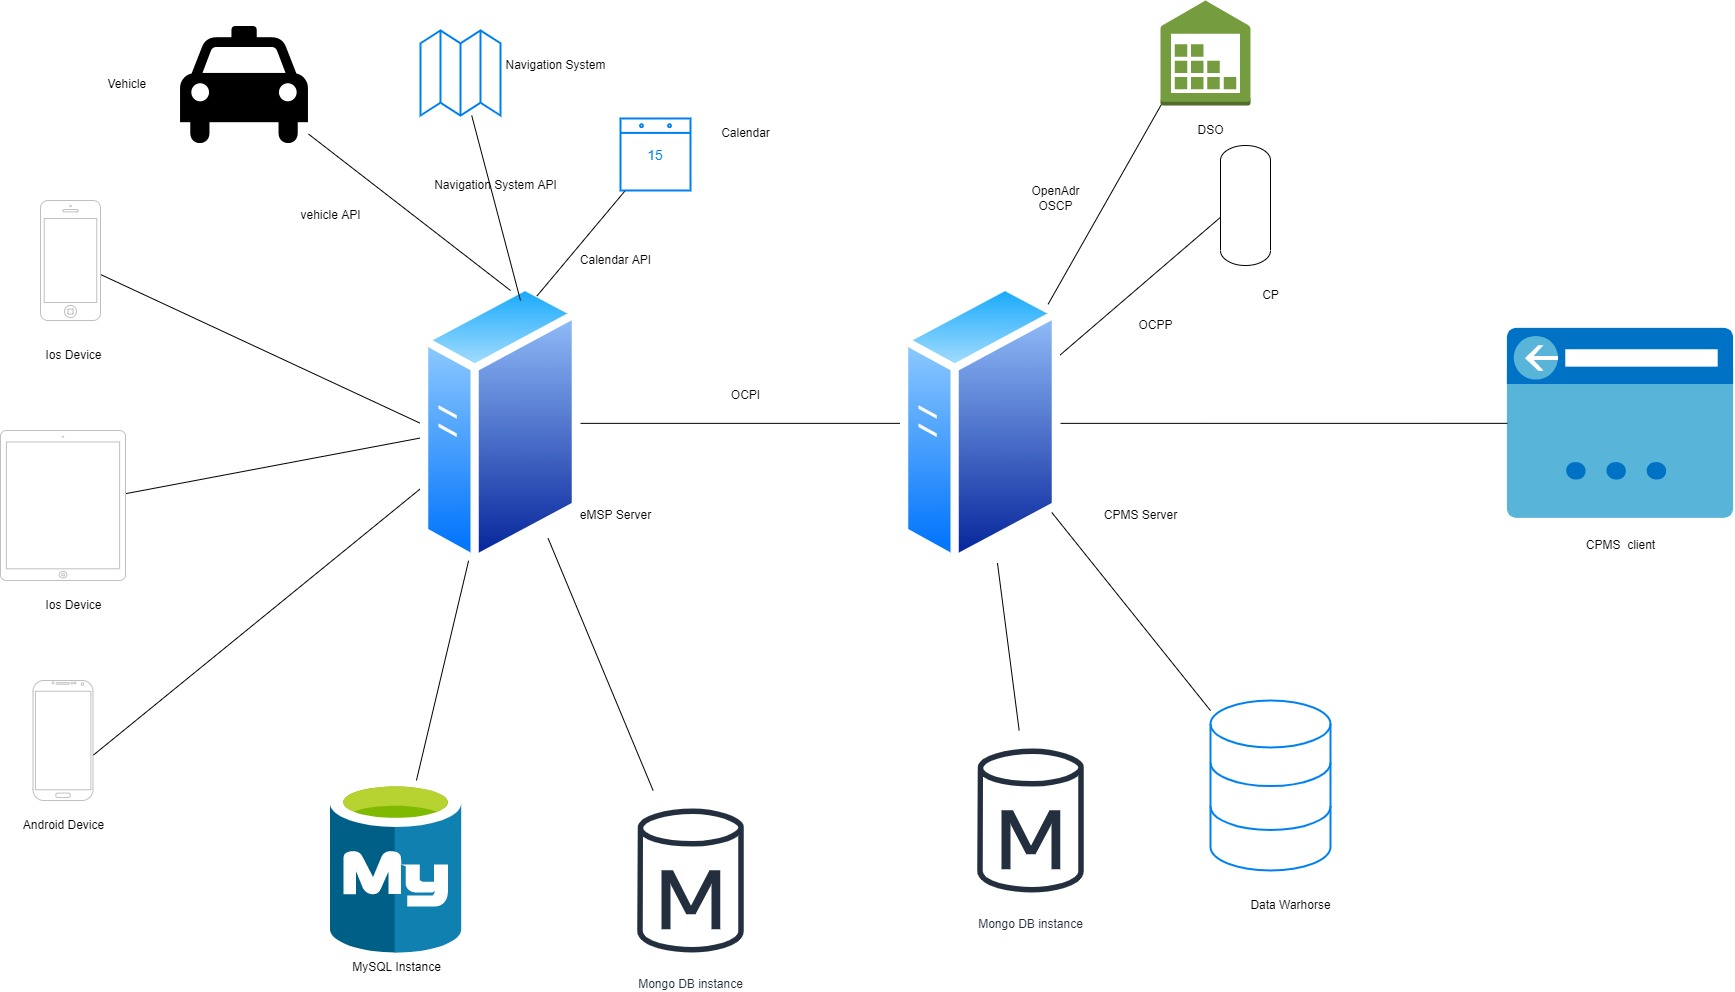
\includegraphics[width=1\textwidth]{Images/high-level/Overview-3.jpg}
    \caption{High level diagram}
\end{figure}

\section{Component View}

\subsection{High level components}

This component diagram shows the high-level components that are involved in the system and the interaction between them and the external systems. The components in Figure~\ref{fig:component-hl} are:

\begin{itemize}
    \item \textbf{eMSP Server}: that contains the business logic of the eMSP and offers its features to the eMSPClientApplication. This component is in charge of interacting with all the external systems through the following APIs:
        \begin{itemize}
            \item \textbf{Mail API}: connects the eMSP Server to the service used to verify the email of the users during the registration
            \item \textbf{Payment Service API}: used for interacting with the payment service, for both processing payments of charging sessions and validating payment methods inserted by users
            \item \textbf{VIN API}: used to validate the vehicles inserted by the users in the application.
            \item \textbf{Calendar API}: used to retrieve the calendar of the user in order to compute suggestions.
            \item \textbf{Navigation System API}: allow the eMSP to interact with the navigation system of the user to compute suggestions.
            \item \textbf{Vehicle API}: connect the eMSP Server to the vehicle in order to retrieve its local and battery status.
        \end{itemize}
    The eMSP Server interact also with the Push Notification Service to send push notifications to the users. In addition, it exposes an OCPI interface to the CPMS that is used to receive updates about the charging points. On the other hand, the eMSP Server uses the OCPI interface of the CPMS to send requests to it.
    \item \textbf{eMSP Client Application}: represents the mobile application installed on the users' devices. It interacts with eMSP Server through the following interfaces:
        \begin{itemize}
            \item \textbf{Station Research Interface}: used to search charging points around a certain position and with a certain distance range
            \item \textbf{Reservation Interface}: used to make reservations in a socket of a charging point and to start charging sessions from an active reservation
            \item \textbf{Charging Session Interface}: used to monitor the status of a charging session and to stop it when it's finished
            \item \textbf{Registration Interface}: used by the unregistered users to create an account in the eMSP
            \item \textbf{Login Interface}: used to login and, at the same time, retrieve the token used for following requests after the login.
            \item \textbf{User Data Interface}: used to view personal data, like vehicles and payment methods, and to modify them.
        \end{itemize}
    \item \textbf{eMSP Users DBMS}: represents the database of the eMSP that is in charge of managing the data of the users (vehicles, reservations, payments, ...).
    \item \textbf{eMSP Charging Points DBMS}: it is the database of the eMSP used to save the location of the charging points and the status of their sockets. The information in this database comes from the updates that the CPMSs send to the eMSP and it is used as a sort of cache to speed up station research.
    \item \textbf{CPMS Server}: contains the entire business logic of the CPMS. It communicates with the CPO through the CPMS Client Application and with the eMSPs through OCPI (for both receiving requests, like reservation making and charging sessions monitoring, and sending updates of the charging points status). The CPMS Server communicates with the charging point through the OCPP interface and with the DSOs with the DSO API (which consists of both the OSCP and the OpenADR interfaces). The CPO Verifier API is used by the CPMS Server to verify the CPO identity during registration and the charging points' existence when a CPO wants to insert a new charging point.
    \item \textbf{CPMS Client Application}: represents the web application through which the CPO can access the CPMS. The CPO can log in to the server through the \textbf{CPO Login Interface} and can register to it through the \textbf{CPO Registration Interface}. The \textbf{CP Status Interface} is used by the CPO to access the information of the status of his charging points and to manage the status of the sockets, the energy sources of a charging point and the tariffs.
    \item \textbf{Business DBMS}: it is the database of the CPMS, used for storing operational data (charging points and sockets status, reservations on sockets, dso offers, ...)
    \item \textbf{CPMS Data Warehouse}: it is the OLAP database of the CPMS, used to make data analytics for both providing better and more fast visualization of historical data to the CPO and for allowing the internal components of the CPMS server to analyse historical data in order to optimize the management of the charging points when in automatic mode.
\end{itemize}

\begin{figure}[H]
    \centering
    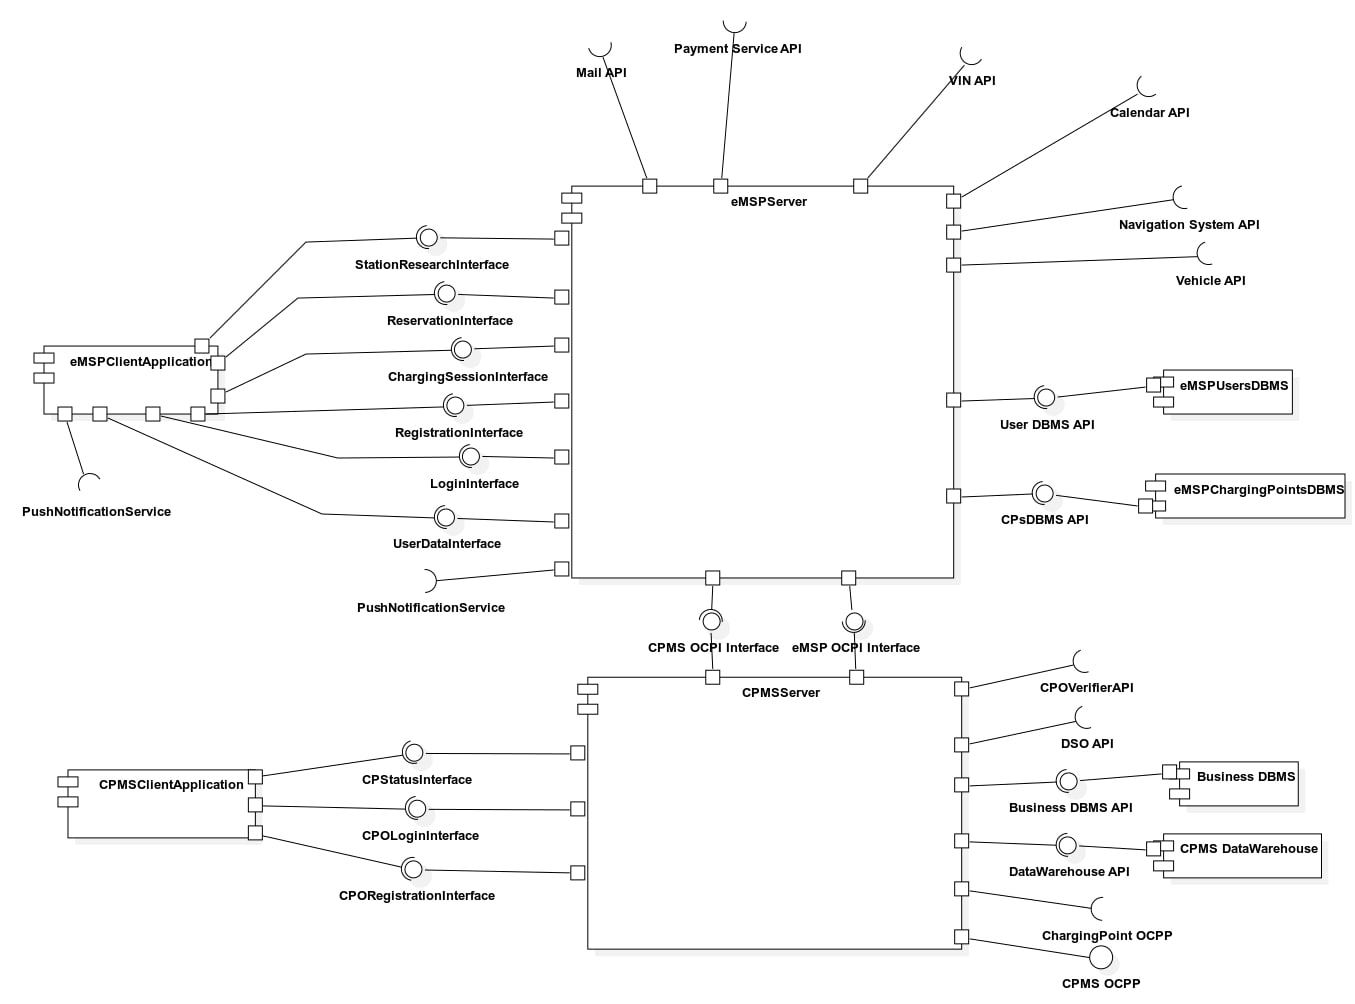
\includegraphics[width=1\textwidth]{Images/component/ComponentDiagram1.jpg}
    \caption{High level components}
    \label{fig:component-hl}
\end{figure}

\subsection{eMSP Server}

In Figure~\ref{fig:component-hl} are represented the internal components of the eMSP Server. Further refinements of some of these components are in the next subsections. 

\begin{figure}[H]
    \centering
    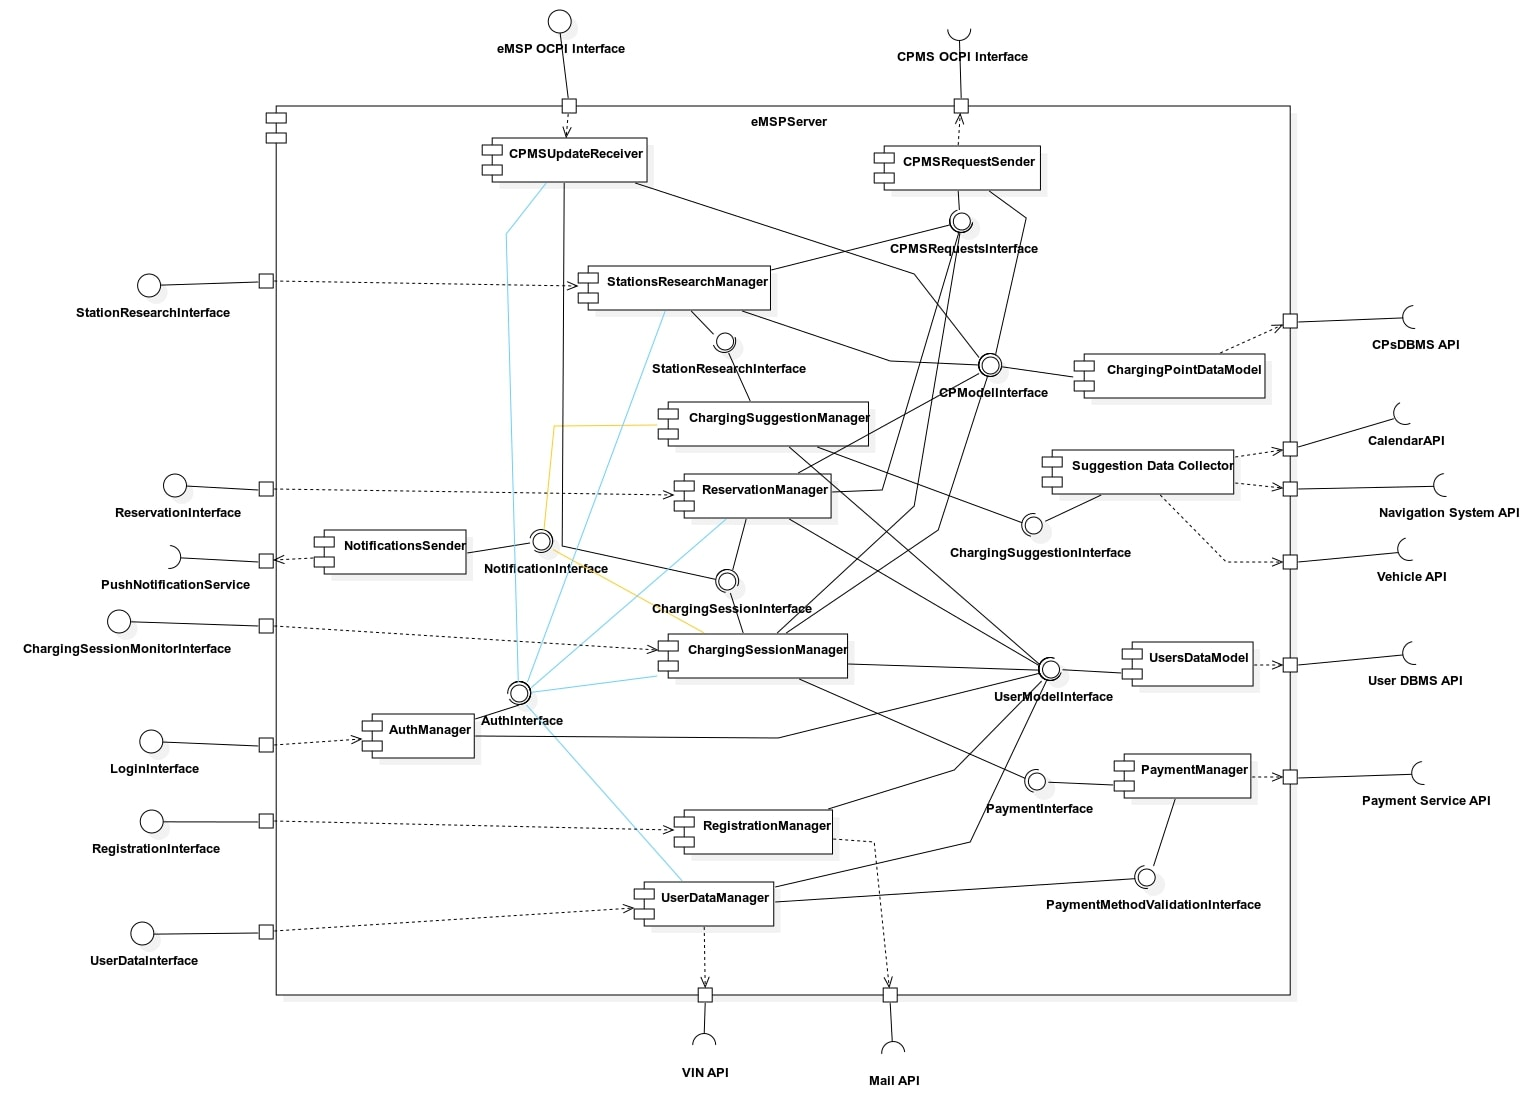
\includegraphics[width=1\textwidth]{Images/component/eMSPServer.jpg}
    \caption{eMSP Server component diagram}
    \label{fig:eMSPServer}
\end{figure}

In this diagram, the components are:
\begin{itemize}
    \item \textbf{Auth Manager}: is the component that handles the login of the users in the eMSP. In addition, it generates the tokens for the users during the login and it verifies the token when logged users make requests to the server. Also, it verifies the identity, through another type of token, of the CPMS when an update arrives from it.
    \item \textbf{Registration Manager}: handles the registration of the user in the system. This component interacts with the Mail service in order to send a confirmation mail to the user during the registration process.
    \item \textbf{User Data Manager}: it is responsible for handling the operations on the user's personal data (vehicles and payment methods).
    \item \textbf{Stations Research Manager}: it is the component used by the users to retrieve the charging points near a certain location with a certain distance range. Also, the Charging Suggestion Manager uses this component in order to retrieve charging points when it has to compute the optimal suggestion.
    \item \textbf{Reservation Manager}: handles all the requests from the users that regard a reservation in order to: make a new reservation, monitor the remaining time until the reservation will expire, cancel an active reservation, and start a charging session from an existing reservation. In order to do so, this component interacts with the CPMS Request Sender.
    \item \textbf{Charging Session Manager}: it is responsible for retrieving the status of a charging session, ending it when the user wants to stop it, and paying for a finished charging session. For the first two functions, this component interacts with the CPMS Request Sender, since the status of the charging session is not saved in the database. In the end, it interacts with the Payment Manager.
    \item \textbf{Payment Manager}: handles the payments of finished charging sessions and verifies the validity of a payment method inserted by the user. In both cases, it interacts with the external payment service.
    \item \textbf{Charging Suggestion Manager}: this component is responsible for computing the suggestions for the users when their favourite vehicle has a low battery. In order to do so, it interacts with the Suggestion Data Collector to retrieve information about the user vehicles, calendar, and navigation system.
    \item \textbf{Suggestion Data Collector}: handles the acquisition of data from external services, that are: the Vehicle API, the Navigation System API, and the Calendar API.
    \item \textbf{Notification Sender}: it is responsible for sending push notifications to the client, through the push notification service.
    \item \textbf{Users Data Model}: represents the users' data on the server and acts as a gateway to the eMSP Users DBMS. Almost every component interacts with it since it is the entry point for the data.
    \item \textbf{Charging Point Data Model}: represents the charging points data on the server and is used by the Stations Research Manager to retrieve charging points and sockets in a certain position and by the Reservation Manager to check the status of a socket before making a reservation.
    \item \textbf{CPMS Request Sender}: sends the HTTP requests to the CPMS. In order to do so it needs to know to which CPMS sends the request, this is why it is connected to the Charging Points Data Model.
    \item \textbf{CPMS Update Receiver}: receive the update from the CPMS that regard the sockets status and the charging session status.
\end{itemize}

\subsubsection{Auth Manager}

\begin{figure}[H]
    \centering
    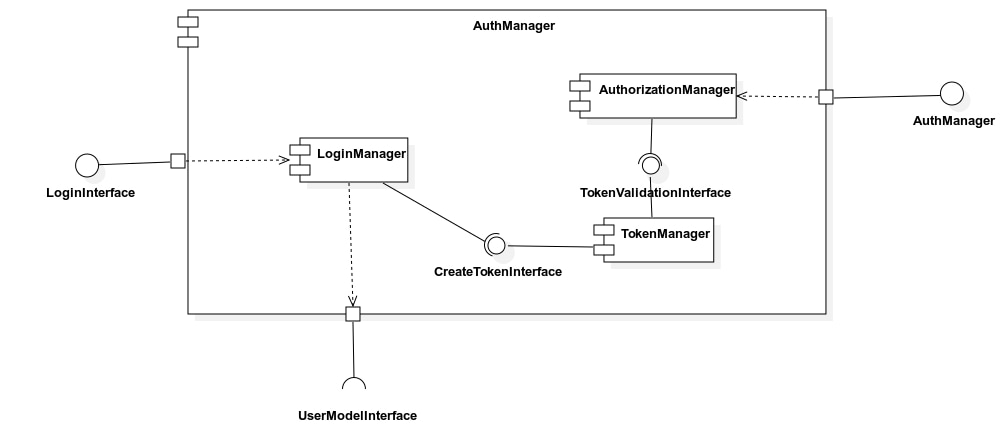
\includegraphics[width=1\textwidth]{Images/component/AuthManager.jpg}
    \caption{Auth Manager component diagram}
\end{figure}

The internal subcomponents of the Auth Manager are:
\begin{itemize}
    \item \textbf{Login Manager}: handles the login of the user and interacts with the Token Manager in order to generate tokens.
    \item \textbf{Token Manager}: manage the tokens of both users and CPMSs. In particular, it verifies the validity and the expiration of a token and generates tokens when a new user is logged in.
    \item \textbf{Authorization Manager}: verifies the permission of the entity (user or CPMS) that sends an HTTP request to the eMSP to perform any requested actions.
\end{itemize}

\subsubsection{User Data Manager}

\begin{figure}[H]
    \centering
    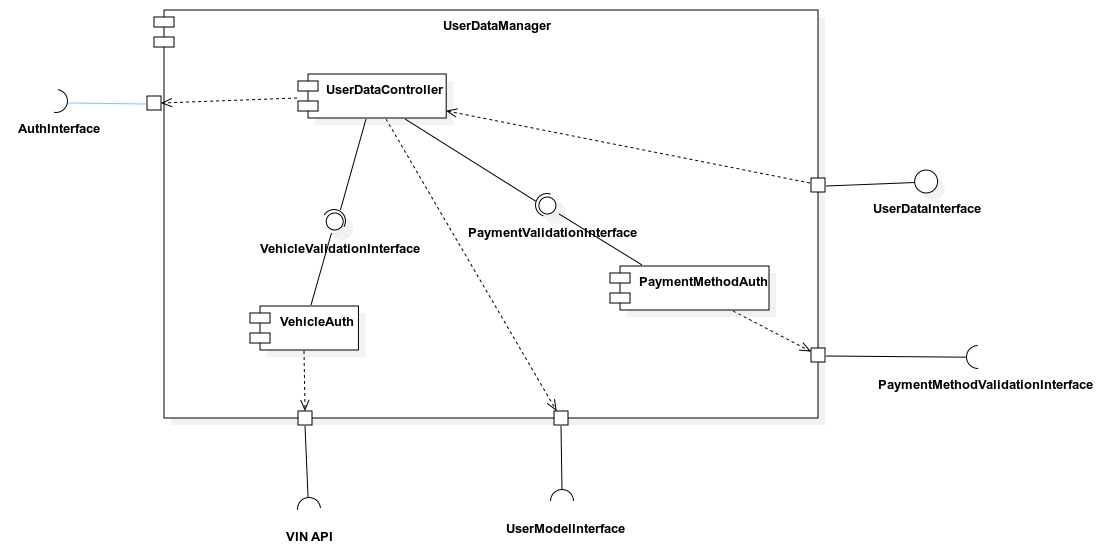
\includegraphics[width=1\textwidth]{Images/component/UserDataManager.jpg}
    \caption{User Data Manager component diagram}
\end{figure}

The internal subcomponents of the User Data Manager are:
\begin{itemize}
    \item \textbf{User Data Controller}: used when users request to view, modify, insert or remove personal data (i.e. vehicles and payment methods).
    \item \textbf{Vehicle Auth}: verifies the existence of a vehicle when the user tries to insert it into the system.
    \item \textbf{Payment Method Auth}: verifies the existence of a payment method when the user tries to add it to his payment methods.
\end{itemize}

\subsubsection{Charging Session Manager}

\begin{figure}[H]
    \centering
    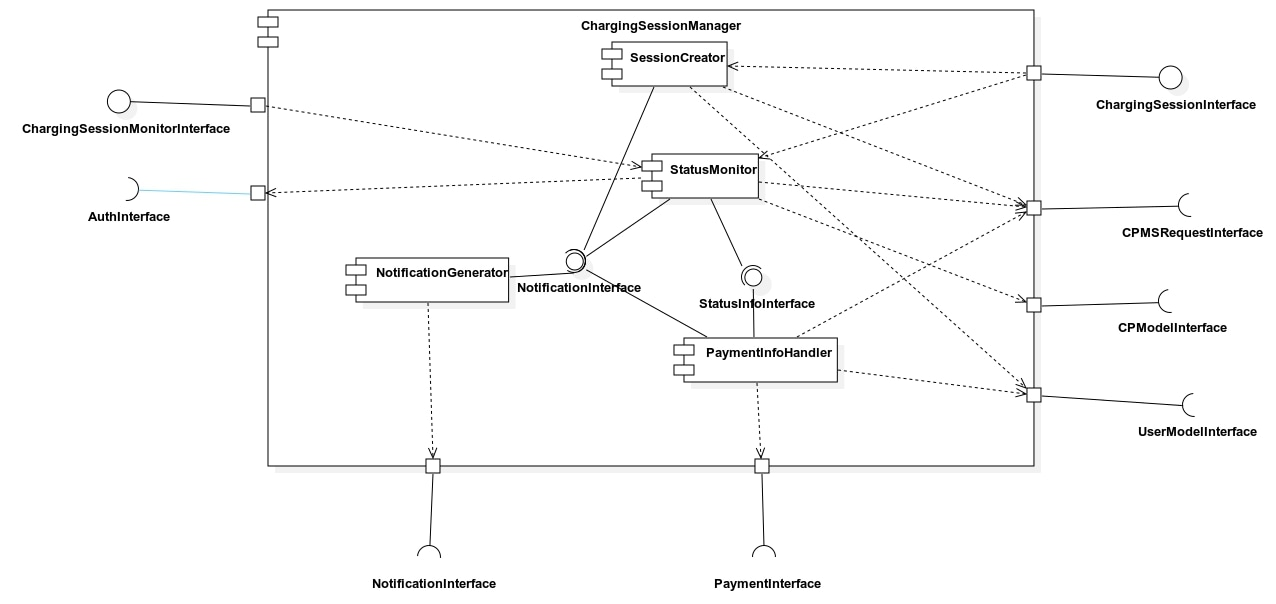
\includegraphics[width=1\textwidth]{Images/component/ChargingSessionManager.jpg}
    \caption{Charging Session Manager component diagram}
\end{figure}

The internal subcomponents of the Charging Session Manager are:
\begin{itemize}
    \item \textbf{Session Creator}: this component is in charge of creating a charging session instance in the database when an update from the CPMS arrives (passing through the CPMS Update Receiver) and of sending a notification (through the Notification Generator) to the user when the session is started.
    \item \textbf{Status Monitor}: offers the user the possibility to monitor the status of an active charging session, to stop a charging session when the battery is full or before it, and to pay for a finished session (through the Payment Info Handler).
    \item \textbf{Payment Info Handler}: handles the payment of a charging session by acquiring the info of the CPO IBAN and by passing the request to the Payment Manager. When the Payment Manager returns the result of the payment, the payment handler sends a notification to the client application through the Notification Generator.
    \item \textbf{Notification Generator}: create a notification and sends it to the user by interacting with the Notification Sender.
\end{itemize}

\subsubsection{Suggestion Data Collector}

\begin{figure}[H]
    \centering
    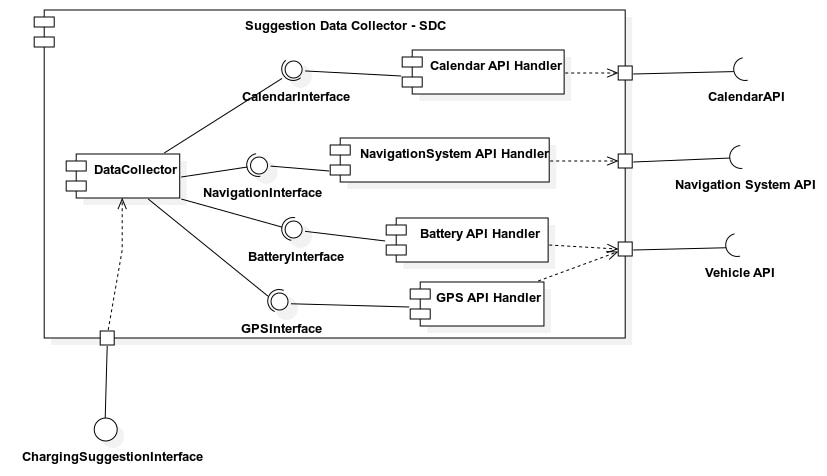
\includegraphics[width=1\textwidth]{Images/component/Suggestion Data Collector.jpg}
    \caption{Suggestion Data Collector component diagram}
\end{figure}

The internal subcomponents of the Suggestion Data Collector are:
\begin{itemize}
    \item \textbf{Data Collector}: handles requests from the Charging Suggestion Manager for retrieving data used to compute the suggestions.
    \item \textbf{Battery API Handler}: retrieves the battery level of a vehicle.
    \item \textbf{GPS API Handler}: retrieves the real-time position of a vehicle.
    \item \textbf{Navigation System API Handler}: retrieves the data from the navigation system of the users.
    \item \textbf{Calendar API Handler}: retrieves the data from the calendar of the users.
\end{itemize}

\subsubsection{Charging Suggestion Manager}

\begin{figure}[H]
    \centering
    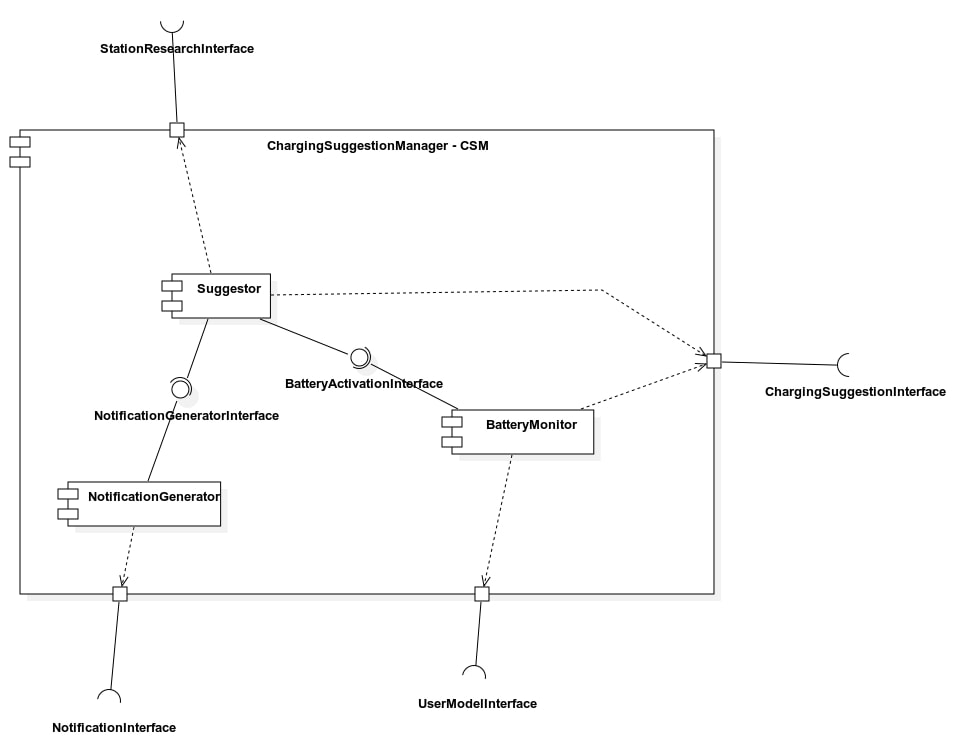
\includegraphics[width=1\textwidth]{Images/component/ChargingSuggestionManager.jpg}
    \caption{Charging Suggestion Manager component diagram}
\end{figure}

The internal subcomponents of the Charging Suggestion Manage are:
\begin{itemize}
    \item \textbf{Battery Monitor}: periodically retrieves the battery of the user's favourite vehicles and notifies the Suggestor when the battery of a vehicle is low.
    \item \textbf{Suggestor}: handles the computation of the optimal suggestion when notified by the Battery Monitor. To do so, it uses the Suggestion Data Collector (through the Charging Suggestion Interface) to retrieve the data about the position of the vehicle, the navigation system info, and the calendar data, and the Stations Research Manager to retrieve the charging points near the position of the vehicle.
    \item \textbf{Notification Generator}: generates the notification for the suggestion that will be sent to the user and uses the Notification Sender to send the notification to the client.
\end{itemize}

\subsection{CPMS Server}

In this diagram (Figure~\ref{fig:cpms-server}) are represented the internal components of the CPMS Server. Further refinements of some of these components are in the next subsections. 

\begin{figure}[H]
    \centering
    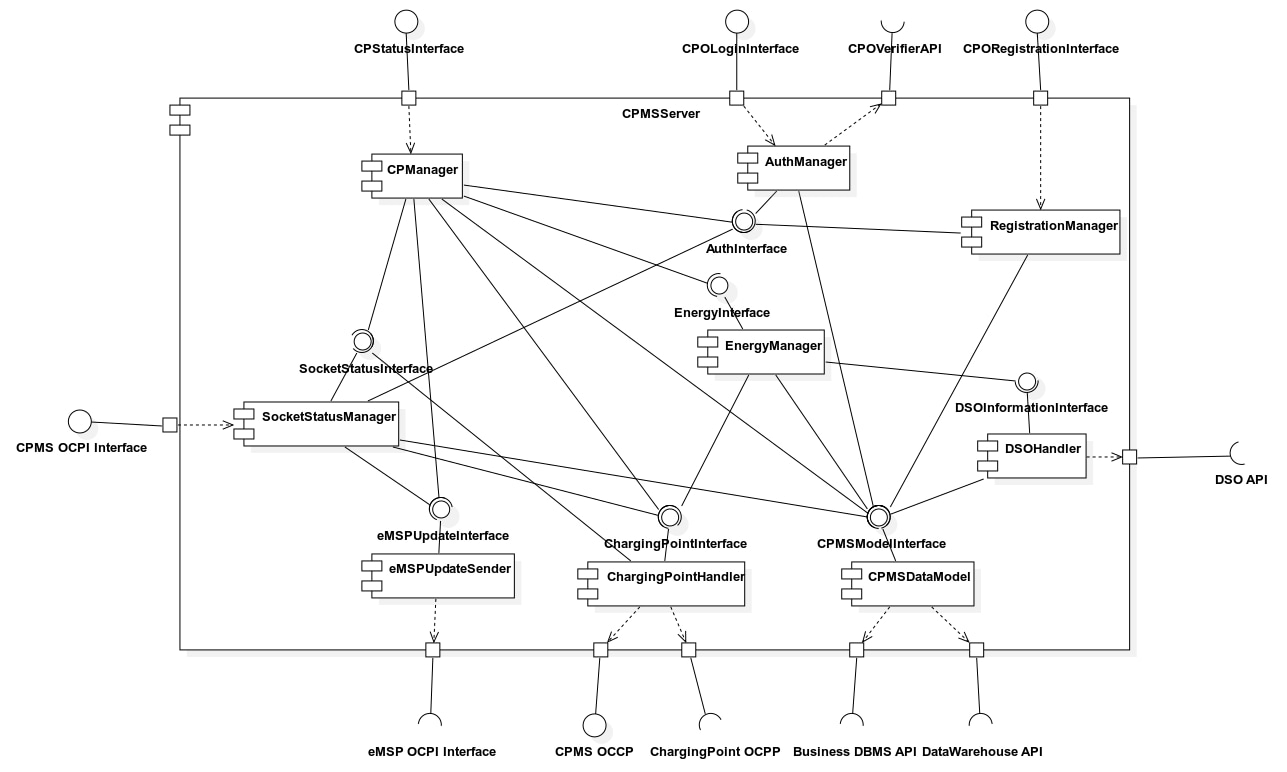
\includegraphics[width=1\textwidth]{Images/component/CPMSServer.jpg}
    \caption{CPMS Server component diagram}
    \label{fig:cpms-server}
\end{figure}

The components of the CPMS Server are:
\begin{itemize}
    \item \textbf{Registration Manager}: allows the CPO to register to the CPMS. The CPO inserts his code to register and the Registration Manager uses the Auth Manager in order to verify that the code refers to an existing CPO.
    \item \textbf{Auth Manager}: handles the login of the CPO, verifies the tokens that CPOs and eMSPs use to make requests to the CPMS, generates tokens for the CPOs when they log in, and verifies both the code that the CPO inserts to register/login and the code that identifies a cp when the CPO tries to add it to the system.
    \item \textbf{CP Manager}: handles all the requests from the CPOs that regard the charging points. Requests that concern the tariff or special offers are handled directly by this component. Requests that concern sockets or energy management are passed, respectively, to the Socket Status Manager and to the Energy Manager. In addition, this component optimizes the tariffs of the charging points, if the charging point is set to automatic mode for price management.
    \item \textbf{Socket Status Manager}: handles the status of the socket. This component receives requests from the eMSPs that can regard a reservation, a charging session, or the status of a socket. In addition, this component provides the CP Manager with information about the status of a socket that will be sent to the CPO when he requests them.
    \item \textbf{Energy Manager}: manages the energy sources and the DSO selection of the charging point. If these functionalities are in manual mode, the component provides the methods to change them to the CPO (passing through the CP Manager that simply receives the requests). If they are in automatic mode, this component is able to optimize independently the selection of the DSO and the management of the energy mix for the charging points.
    \item \textbf{DSO Handler}: periodically acquires the offers from the DSOs and stores them in the database for further needs, so if the CPO or the Energy Manager needs them, they are already stored and ready to be read (and analyzed in case of the Energy Manager). If a DSO changes its offer the DSO Handler will notify the Energy Manager, that will recompute the selection of the DSO if the functionality is in automatic mode.
    \item \textbf{eMSP Update Sender}: sends the socket and charging session status updates to the eMSPs. In particular, every time a socket changes its status, every connected eMSP is notified by this component. Regarding charging sessions, an update is sent to the eMSP only when the session is started or the battery of the car is full. In all other cases, it is the eMSP that needs to request the status to the Socket Status Manager.
    \item \textbf{Charging Point Handler}: manages the interaction with the charging point (receiving and sending updates) through the OCPI protocol.
    \item \textbf{CPMS Data Model}: is the representation of the data in the CPMS Server. It retrieves the data both from the Business DBMS and from the Data Warehouse.
\end{itemize}

\subsubsection{CP Manager}

\begin{figure}[H]
    \centering
    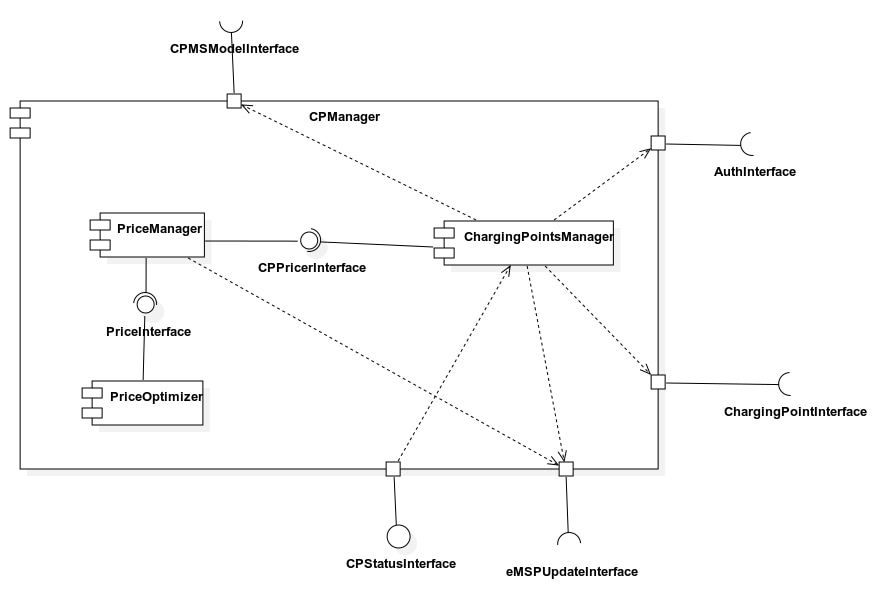
\includegraphics[width=1\textwidth]{Images/component/CPManager.jpg}
    \caption{CP Manager component diagram}
\end{figure}

The internal subcomponents of the CP Manager are:
\begin{itemize}
    \item \textbf{Charging Points Manager}: is the main component for managing the charging points. This component receives all requests from the CPO (and therefore it needs to interact with the Auth Manager in order to identify the CPO) regarding charging points and then it passes them to the correct component. In addition, this component also manages directly the insertion of a new charging point in the system, with the help of the Auth Manager for verifying the existence of the charging point.
    \item \textbf{Price Manager}: handles the tariffs and the special offers for the charging points. If the price management functionality is set to automatic mode for a certain charging point, it uses the price optimizer to compute the best tariffs and to set some special offers when it seems convenient.
    \item \textbf{Price Optimizer}: handles the optimization process of the tariffs and special offers. To do so, it has to access the data in the Data Warehouse.
\end{itemize}

\subsubsection{Socket Status Manager}

\begin{figure}[H]
    \centering
    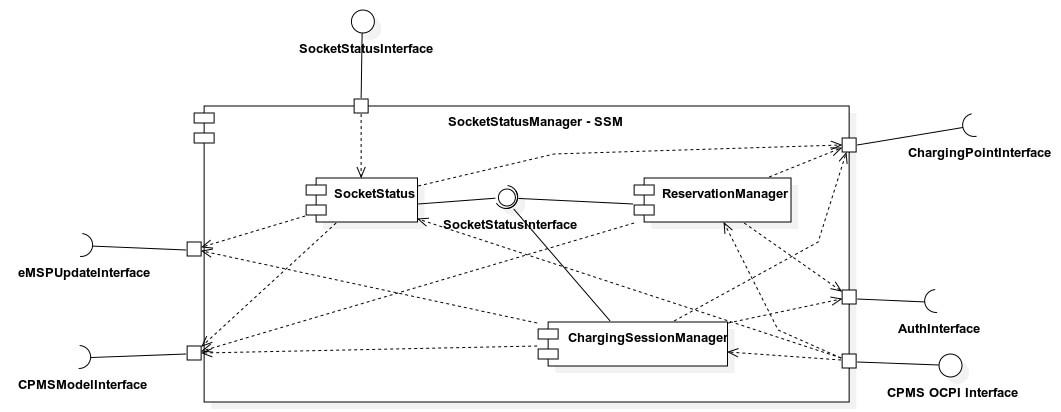
\includegraphics[width=1\textwidth]{Images/component/SocketStatusManager.jpg}
    \caption{Socket Status Manager component diagram}
\end{figure}

The internal subcomponents of the Socket Status Manager are:
\begin{itemize}
    \item \textbf{Socket Status}: receive the request from the eMSPs that regards the status of the sockets. In addition, provides the CPO (through the CP Manager) information about the status of the sockets and the charging sessions and the possibility to change the availability of a socket (for example if it has to be put in maintenance). When a socket changes its status, this component uses the eMSP Update Interface of the eMSP Update Sender in order to inform all the eMSPs.
    \item \textbf{Reservation Manager}: handles requests from the eMSPs that regard the reservations on the sockets and forward them to the charging point, using the Charging Point Handler.
    \item \textbf{Charging Session Manager}: handles requests from the eMSPs that regard charging sessions in order to start a charging session from an existing reservation, stop a charging session and monitor the status of the charging session. This component uses the eMSP Update Sender through the eMSP Update Interface in order to inform an eMSP when the battery of a connected vehicle is full or when the energy flow of a charging session has started.
\end{itemize}
All these components modify the Data Model when there are updates of sockets, reservations, and charging sessions. The updates that Charging Session Manager sends to the CPMS Data Model are also used to insert data in the Data Warehouse in order to save historical data about the charging sessions.

\subsubsection{Energy Manager}

\begin{figure}[H]
    \centering
    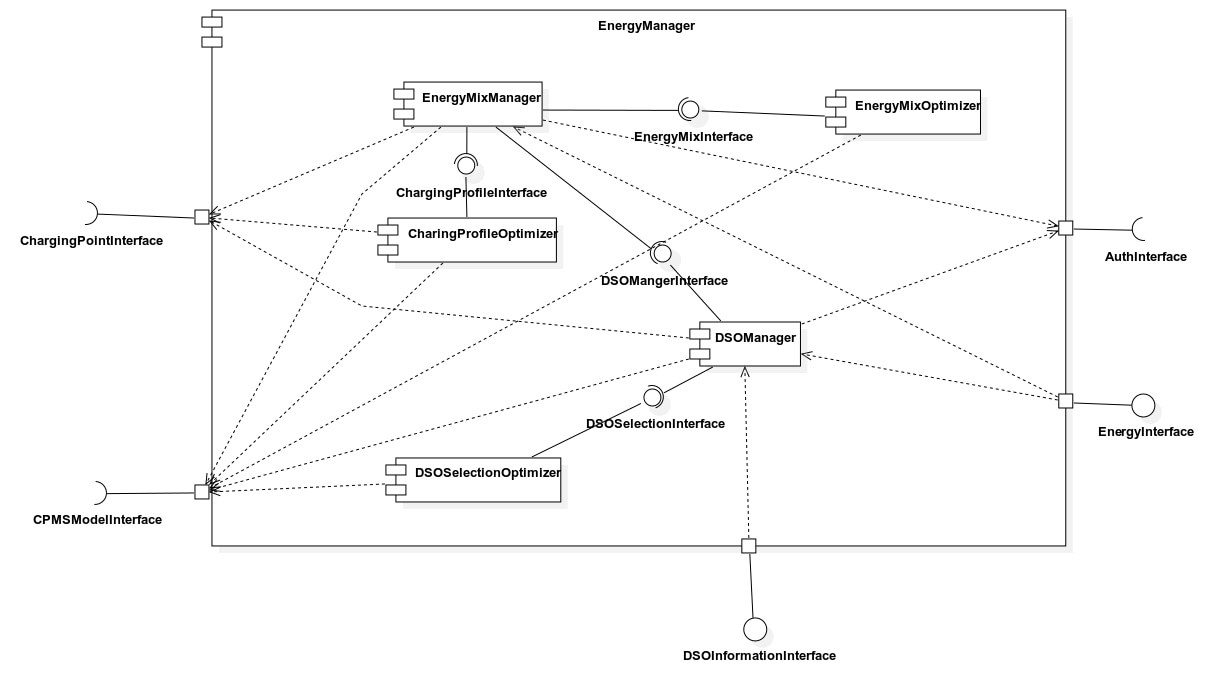
\includegraphics[width=1\textwidth]{Images/component/EnergyManager.jpg}
    \caption{Energy Manager component diagram}
\end{figure}

The internal components of the Energy Manager are:
\begin{itemize}
    \item \textbf{DSO Manager}: handles the request of the CPO (passed from the CP Manager) that concern the DSO, from the retrieval of current offers of energy to manual the selection of the DSO. When a DSO of a charging point changes, it informs the Charging Point through the Charging Point Handler (using the Charging Point interface). When the DSO selection is in automatic mode, it uses the DSO Selection Optimizer to optimize this process.
    \item \textbf{DSO Selection Optimizer}: chooses the best DSO for the charging points, when this functionality is in automatic mode for those charging points. In order to do so, it needs to access data from the Data Warehouse to make the analysis of historical data.
    \item \textbf{Energy Mix Manager}: handles the requests from the CPO that regard the management of the energy mix for the charging points, including the retrieval of the current configuration for a charging point and the manual modification of it by the CPO. When the energy mix is changed, it informs directly the Charging Point, using the Charging Point Handler. If the energy mix management is in automatic mode, this component uses the Energy Mix Optimizer in order to compute the best energy mix.
    \item \textbf{Energy Mix Optimizer}: compute the best energy mix when this functionality is in automatic mode.
    \item \textbf{Charging Profile Optimizer}: compute the most efficient charging profile for the sockets of the charging points. This component is triggered every time the energy mix configuration is changed.
\end{itemize}

\subsection{ER Models}

\subsubsection{eMSP ER Model}

Figure~\ref{fig:emsp-er} represents the model of the data that is stored on both the eMSP Users DBMS and the eMSP Charging Points DBMS. The data is split in these two databases since there are different needs that suit better on different types of databases from the logical point of view:
\begin{itemize}
    \item For the personal data of the users a relational database is more appropriate since users' data will require many joins that involve many different types of entities. In addition, relational databases enforce data integrity constraints, which helps to ensure the accuracy and consistency of the data and this is important for the data of the users.
    \item For the data regarding charging points, that is updated through the notifications that arrive from the CPMS, usually a query requires to retrieve all the information regarding a charging point. In this sense, a documental approach is more appropriate since it has a better data locality.
\end{itemize}

\begin{figure}[H]
    \centering
    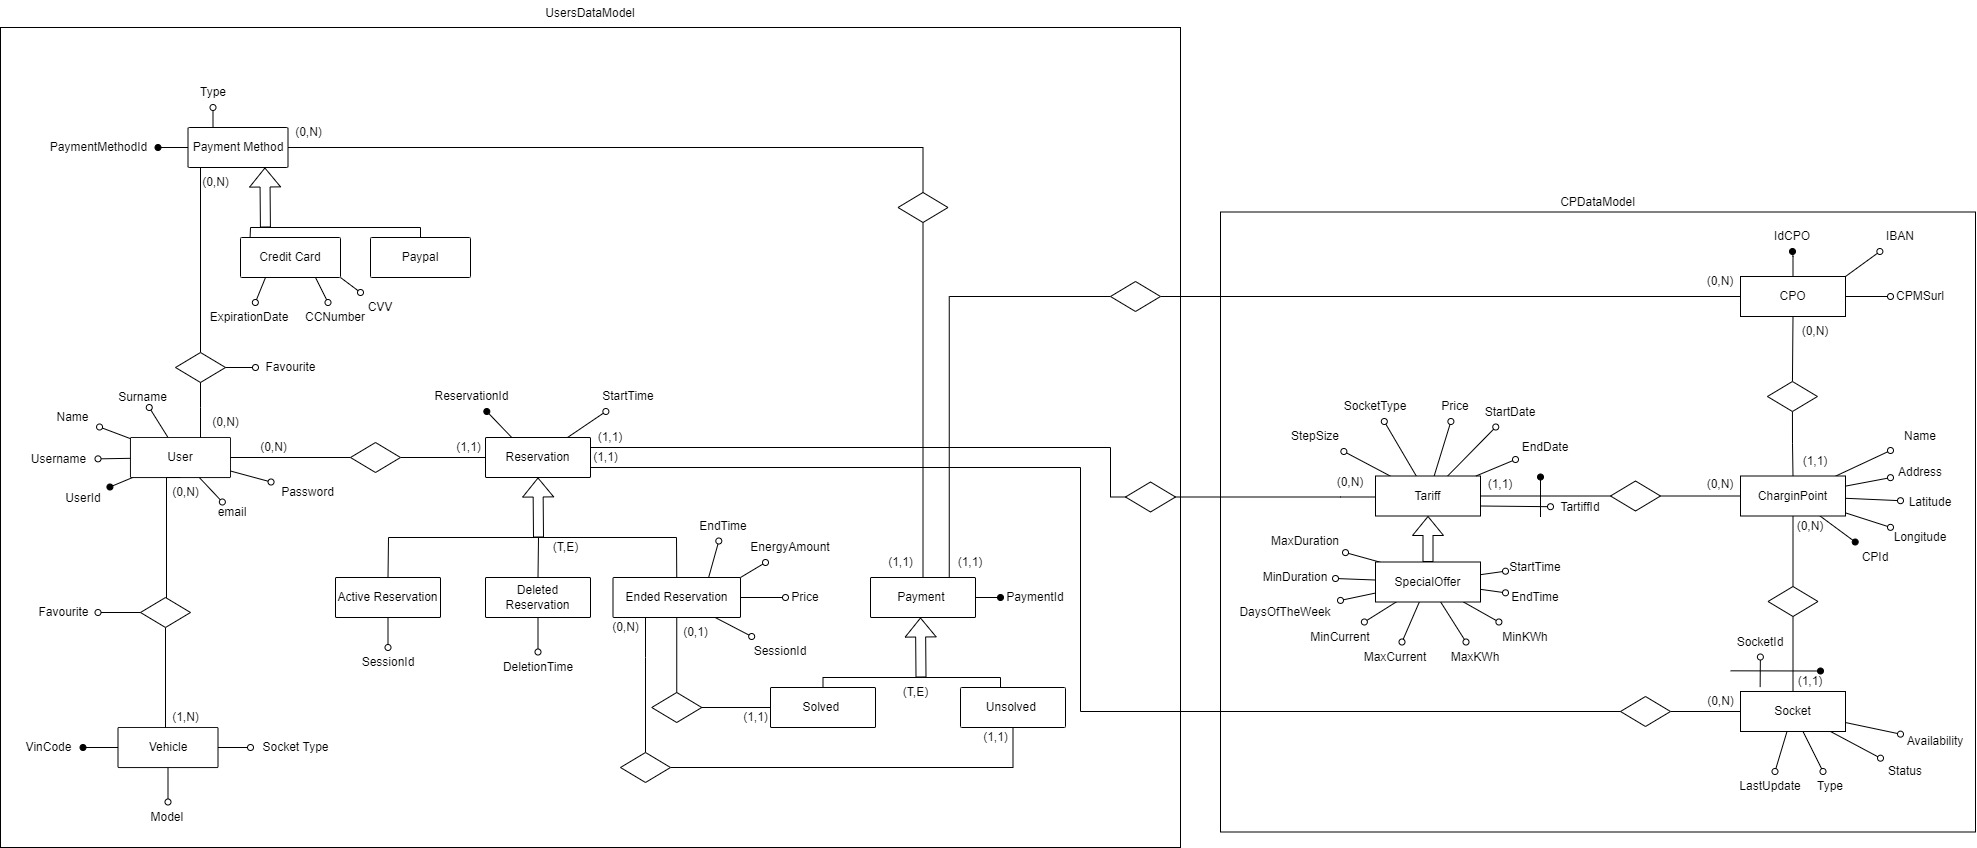
\includegraphics[width=1\textwidth]{Images/er-models/emsp_data_model.jpg}
    \caption{ER Model of the eMSP Databases}
    \label{fig:emsp-er}
\end{figure}

\subsubsection{CPMS ER Models}

Figure~\ref{fig:cpms-business-er} shows how data is represented in the Business database. The selected logical approach to store the data, in this case, is the documental approach since data locality is a very important feature for speeding up the queries since there are many weak entities of the charging point that are usually all retrieved together when information about the charging point is needed.

\begin{figure}[H]
    \centering
    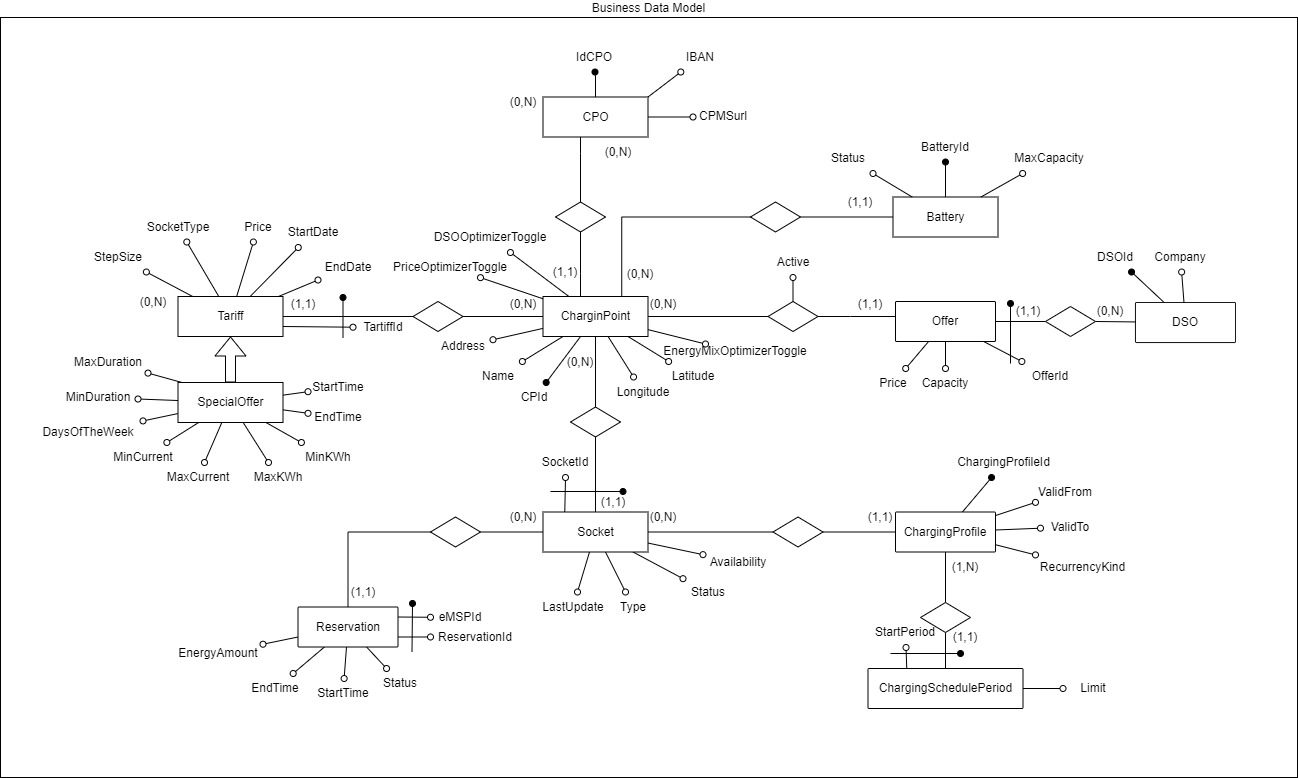
\includegraphics[width=1\textwidth]{Images/er-models/business_data_model.jpg}
    \caption{ER Model of the CPMS OLTP Database}
    \label{fig:cpms-business-er}
\end{figure}

Figure~\ref{fig:cpms-olap-er} represents the model of the data stored in the Data Warehouse of the CPMS. This model follows the snowflake data model usually used to represent the data in a Data Warehouse. There are three types of facts that will be analyzed: the price the dso offers, the energy consumed by a charging point, and the energy consumed and the price paid for a charging session. These facts might be analyzed from different dimensions, which can have different levels of granularity. The data contained in this OLAP database can be seen as a multidimensional cube, where the cells are the measures of the facts and the dimensions of the cube are the dimensions of analysis of the fact. In order to logically store this type of data, a columnar approach fit well since it permits to compression of repeated values of columns, retrieving measures of facts based on ranges of these values, and changing the granularity of the dimensions in an efficient way when analyzing data.

\begin{figure}[H]
    \centering
    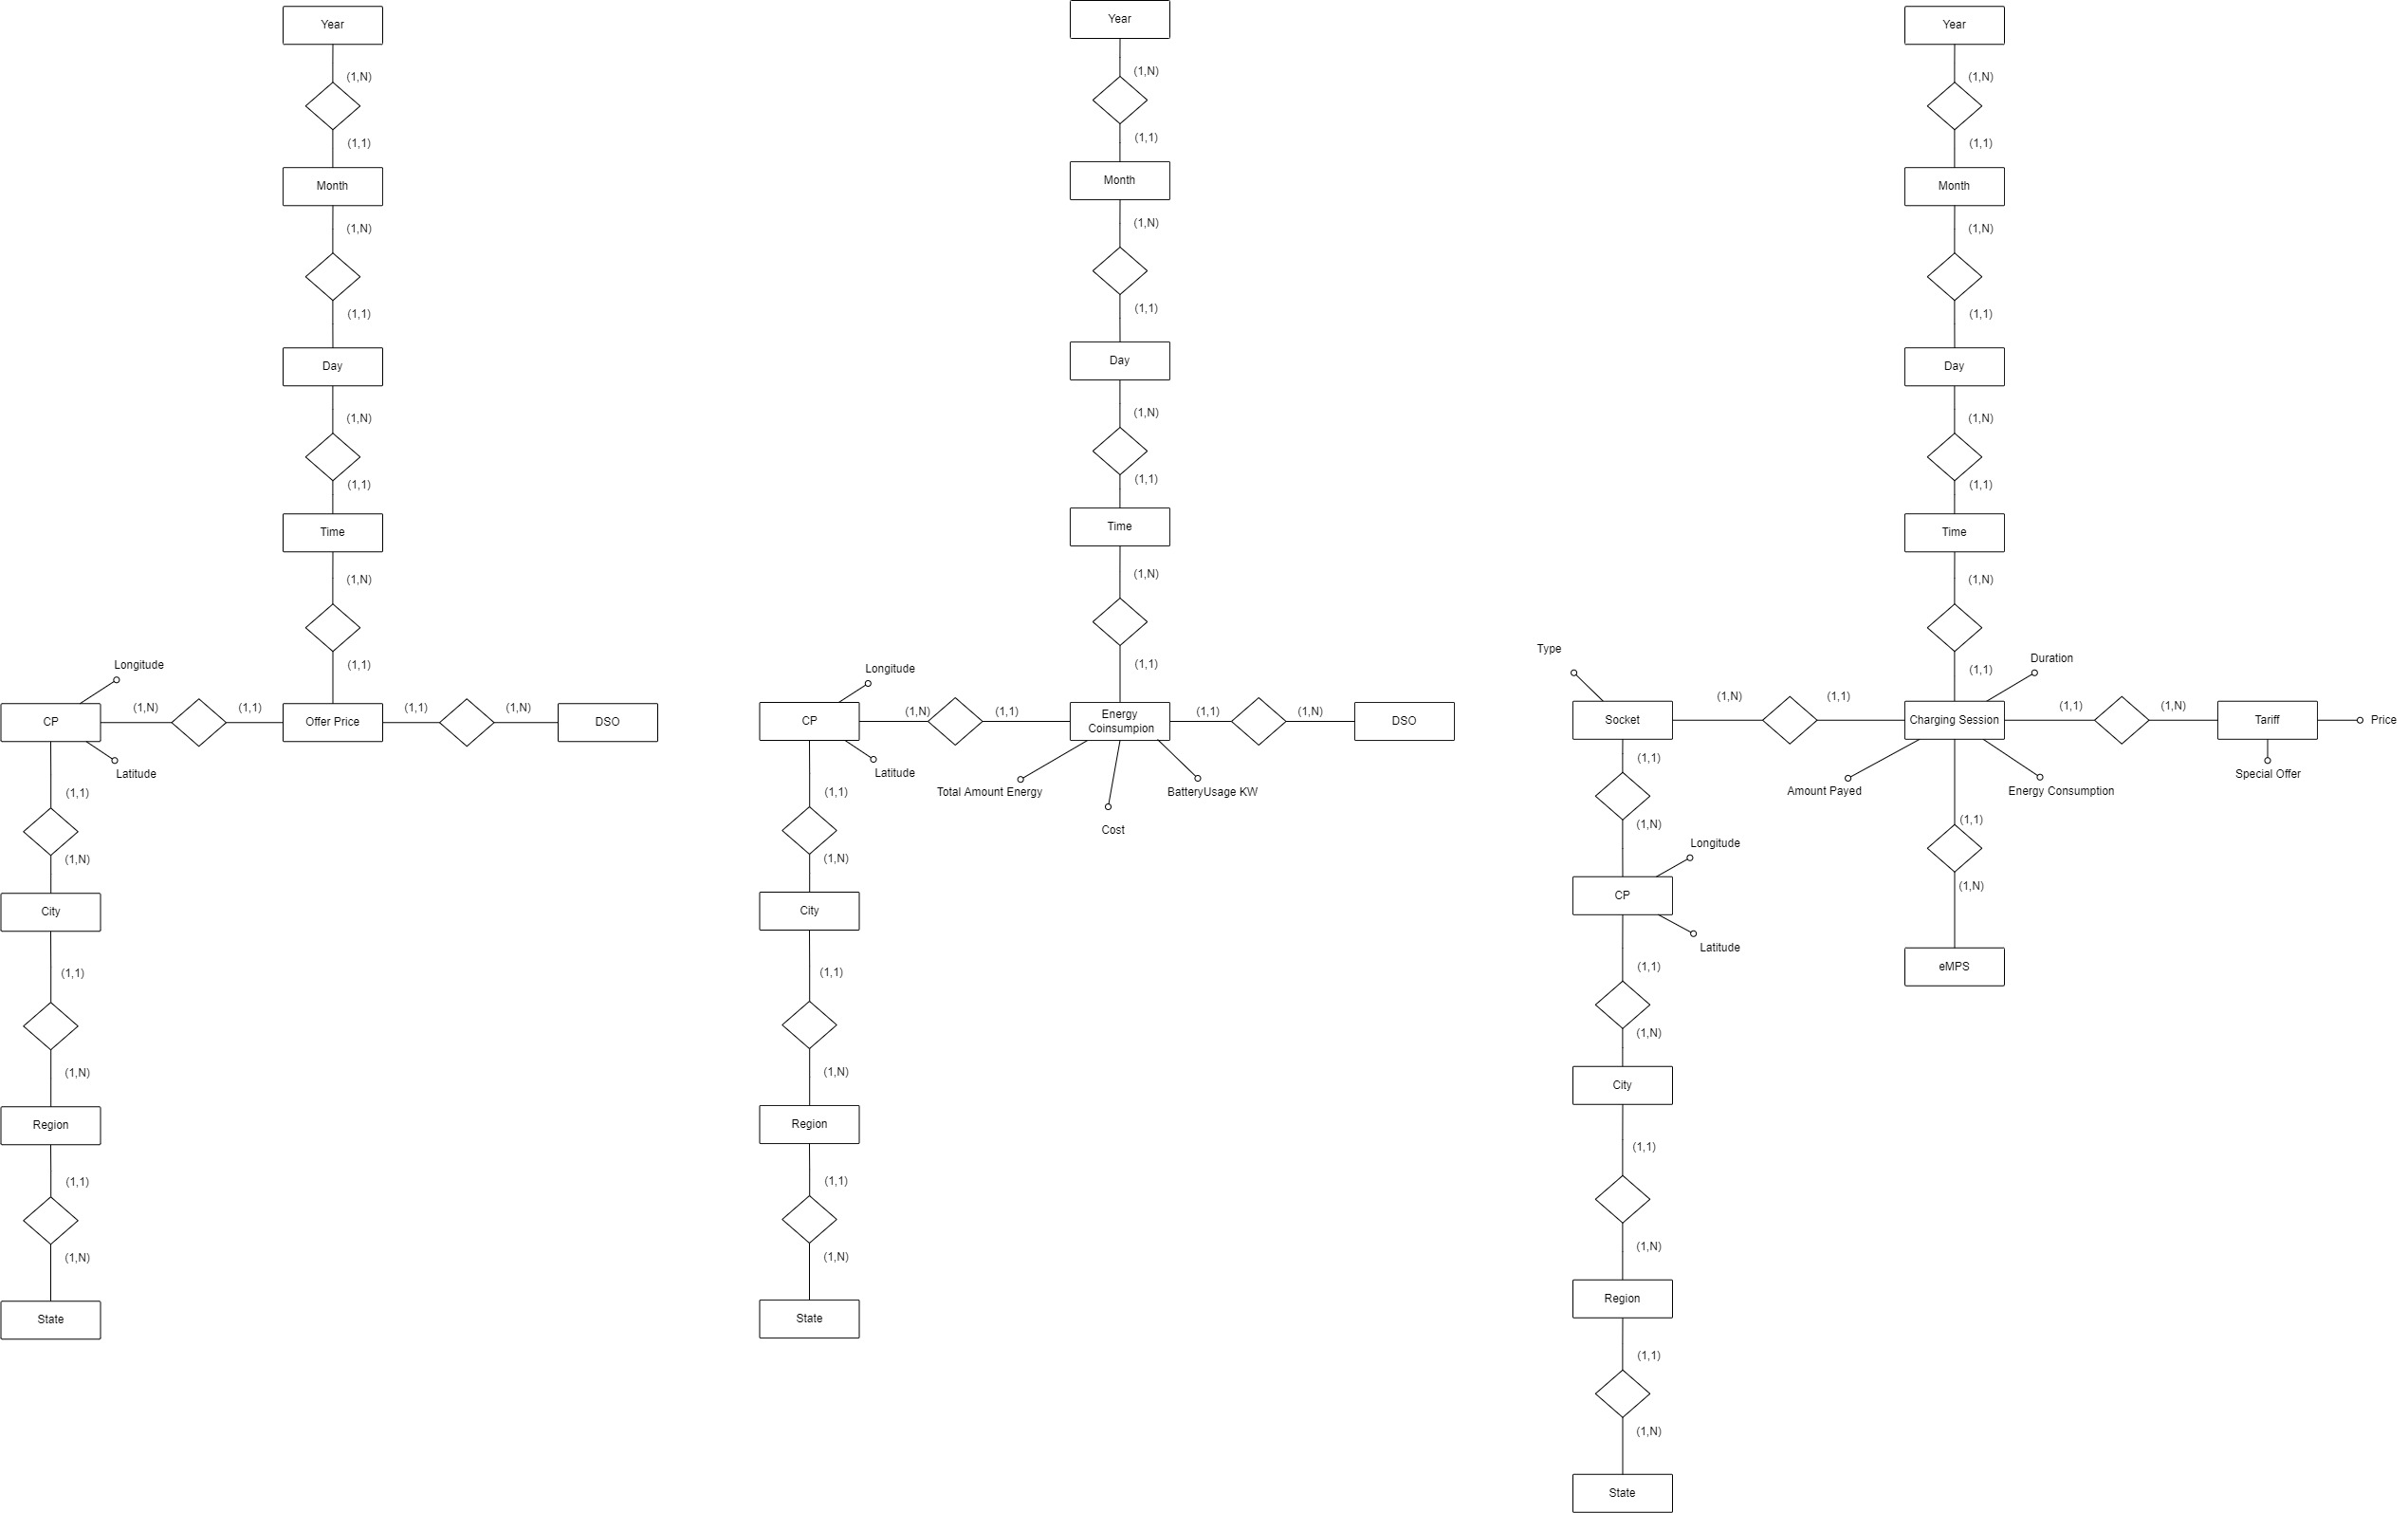
\includegraphics[width=1\textwidth]{Images/er-models/data_warehouse.jpg}
    \caption{ER Model of the CPMS OLAP Database}
    \label{fig:cpms-olap-er}
\end{figure}

\section{Deployment View}

The deployment diagram in Figure~\ref{fig:deploy} shows how the components of both the eMSP and CPMS are deployed. Both systems present a Three-Tier architecture, a software design pattern that divides an application into three logical tiers: the presentation tier, the application logic tier, and the data storage tier. For the eMSP:
\begin{itemize}
    \item The presentation tier is represented by the eMSP Client installed on the mobile phone of the users. It communicates with the Business Logic tier through HTTPS
    \item The business logic tier is represented by the eMSP Application Server on which the eMSP Server is installed. This tier contains multiple replicas of the application to handle many concurrent requests from clients. In order to manage these requests, a Load Balancer is used to assign the proper replica to a request. This tier communicates with the data tier through TCP/IP.
    \item The data tier is represented by the eMSP Database Server on which the data is stored in a persistent way. In this tier, both the eMSP Users Database and the eMSP Charging Points Database are running. The first one runs on an instance of MySQL, which is a very popular relational database and is very reliable and easy to use. The second one runs on an instance of MongoDB, which is a popular documental DB that provides easy-to-use APIs that make it straightforward to access and manipulate data. In addition, with MongoDB, there is the possibility of sharding on the range of values of keys (for example positions of charging points), and this can speed up the queries for station research.
\end{itemize} 
For the CPMS:
\begin{itemize}
    \item The presentation tier is represented by the personal computer of the CPO that runs the CPMS web application on a browser. It communicates with the Business Logic tier through HTTPS.
    \item The business logic tier is represented by the CPMS Application Server on which the CPMS Server is installed. This tier communicates with the data tier through TCP/IP.
    \item The data tier is represented by the CPMS Business Database Server and by the CPMS Data Warehouse Server. The first contains all the data regarding charging points and runs on an instance of MongoDB. The second one contains an instance of Cassandra, which is a database that provides a scalable way of managing historical data of huge dimensions for OLAP databases by mixing the columnar approach and the key-value approach. This server is partitioned and replicated many times since it might contain a huge amount of data. In this sense, Cassandra provides a way to automatically manage the various partitions/replicas of the data.
\end{itemize}
The CPMS Application Server and the eMSP Application Server can communicate using the OCPI protocol, which runs on top of the HTTP protocol. The CPMS Application Server communicates also with the Charging Points through OCPP, which uses the WebSocket, and with the DSOs through both OSCP and OpenADR, which are built on top of HTTP. In addition, the eMSP Application Server communicates with external CPMSs and the CPMS Application Server communicates with external eMSPs. These (the external eMSPs and CPMSs, the Charging Points and the DSOs) are not represented in this diagram because they are out of its scope.
All the HTTPS requests from clients go through Firewalls to have more secure access from the external network. In addition, a Firewall is also present between the business logic tier and the data tier; in this way we are constructing a Demilitarized Zone (DMZ) to have more secure access to the data.

\begin{figure}[H]
    \centering
    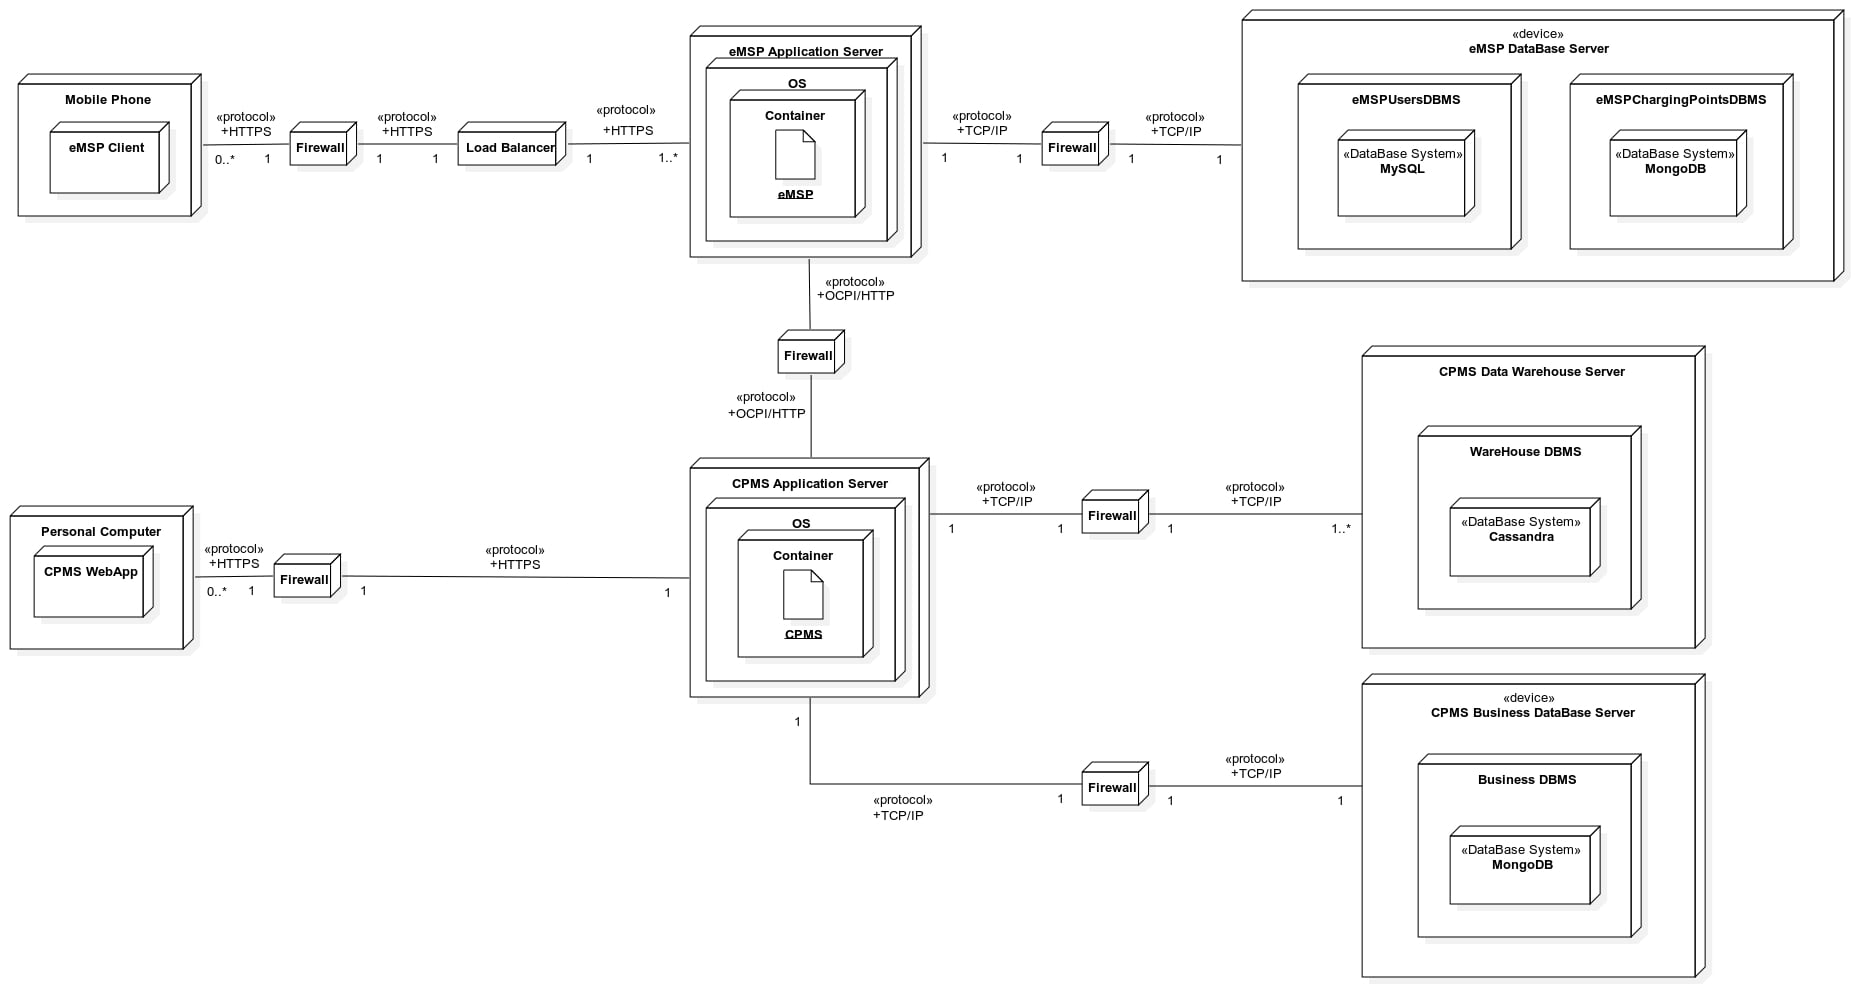
\includegraphics[width=1\textwidth]{Images/deployment/DeploymentDiagram.jpg}
    \caption{Deployment diagram}
    \label{fig:deploy}
\end{figure}

\newpage
\section{Runtime View}

\subsection{User Registration}
\begin{figure}[H]
    \centering
    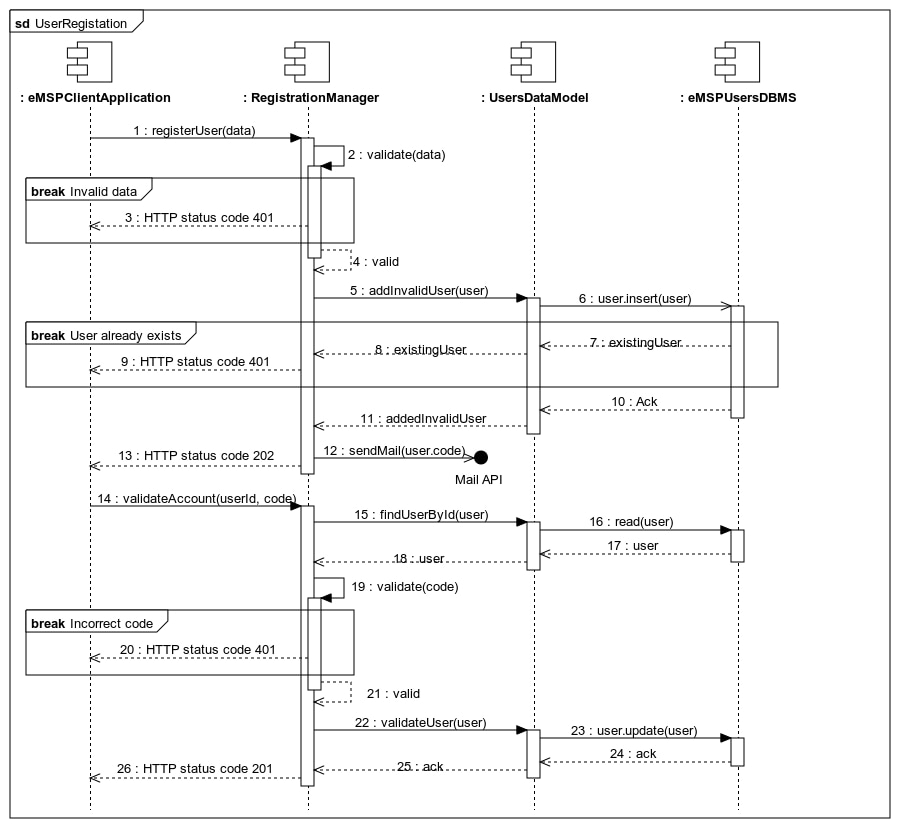
\includegraphics[width=0.8\textwidth]{Images/sequenceDiagrams/UserRegistation.jpg}
    \caption{User Registration}
\end{figure}
The user registration must be confirmed by a code sent to the provided email. Before the confirmation, the user is saved in the database as invalid, and only when the code is correctly inserted, becomes valid and allowed to use the eMSP functions.

\subsection{User Login}
\begin{figure}[H]
    \centering
    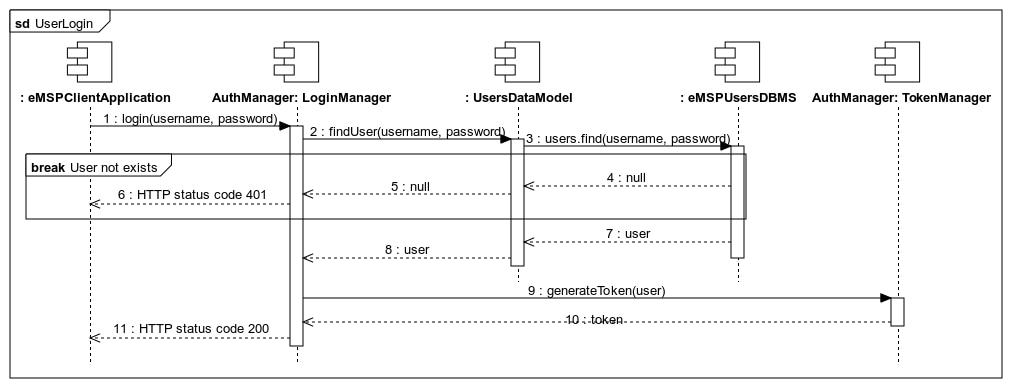
\includegraphics[width=1\textwidth]{Images/sequenceDiagrams/UserLogin.jpg}
    \caption{User Login}
\end{figure}
When the user tries to log into the system, it verifies if the user actually exists. If so, the server generates a unique token used as the identifier for the subsequent requests.

\subsection{Add Vehcile}
\begin{figure}[H]
    \centering
    \includegraphics[width=1\textwidth]{Images/sequenceDiagrams/addVehicle.jpg}
    \caption{Add Vehicle}
\end{figure}
In this diagram, we have an example of how the validation of the token works, sending a negative response to the Client Application when the token is expired, invalid, or if the user is not allowed to use that function.
If the token is valid, the request is taken over by the server that through an external API verifies the validity of the VIN code provided by the user, and then adds the vehicle to the database.

\subsection{Set Favourite Vehcile}
\begin{figure}[H]
    \centering
    \includegraphics[width=1\textwidth]{Images/sequenceDiagrams/setFavoriteVehicle.jpg}
    \caption{Set Favourite Vehicle}
\end{figure}
When the user wants to set the favourite vehicle, useful for the suggestions and filtration of the CPs, the server must update the eventual old one removing the favourite value to it, and setting it to the new one.

\subsection{Remove Vehcile}
\begin{figure}[H]
    \centering
    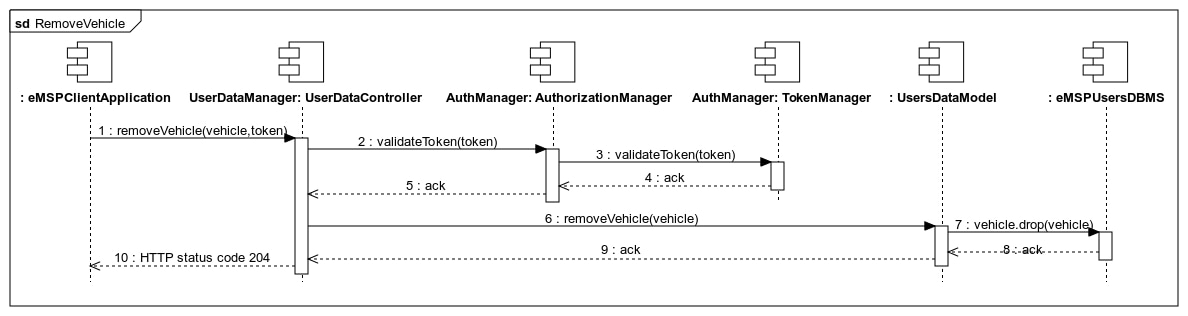
\includegraphics[width=1\textwidth]{Images/sequenceDiagrams/RemoveVehicle.jpg}
    \caption{Remove Vehicle}
\end{figure}
When the user tries to remove a vehicle the system checks the validity of the user through the token and then drops that vehicle from the database.

\subsection{Add Payment Method}
\begin{figure}[H]
    \centering
    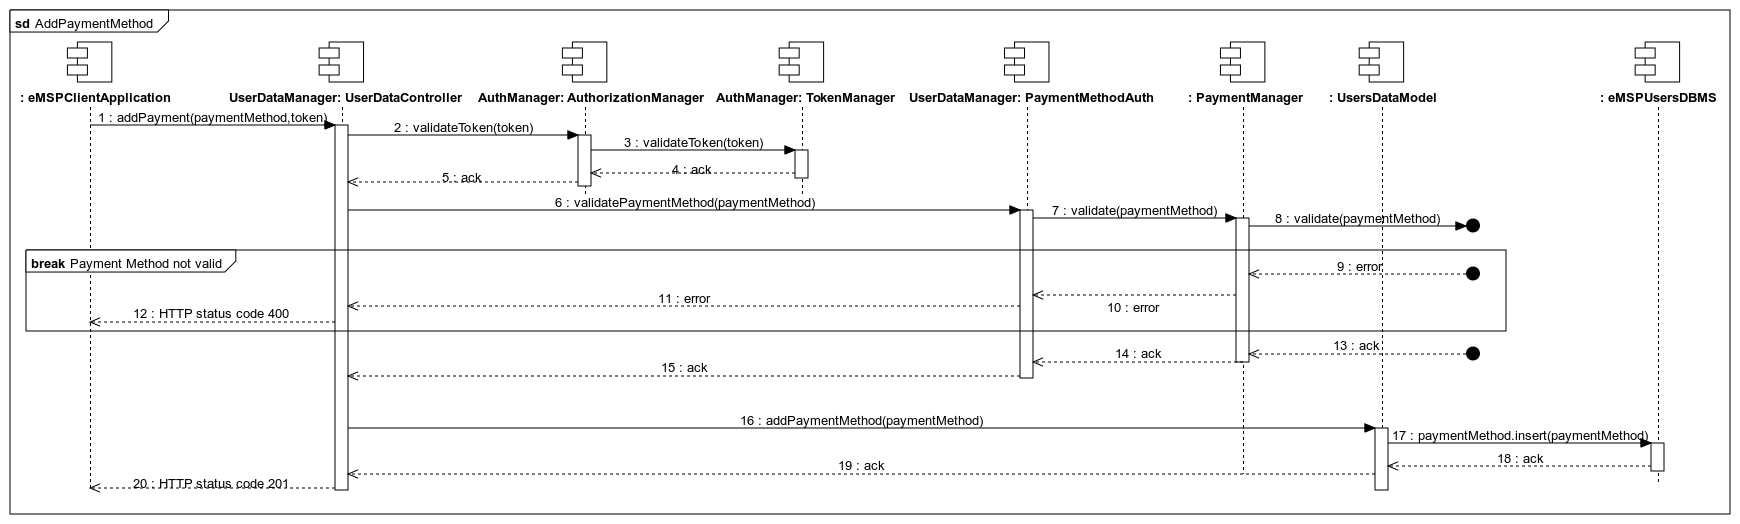
\includegraphics[width=1\textwidth]{Images/sequenceDiagrams/AddPaymentMethod.jpg}
    \caption{Add Payment Method}
\end{figure}
When a user adds a new payment method, the system verifies its validity through an external API, if the response is positive, it is saved in the database so can be retrieved when a user has to pay for the service.

\subsection{Remove Payment Method}
\begin{figure}[H]
    \centering
    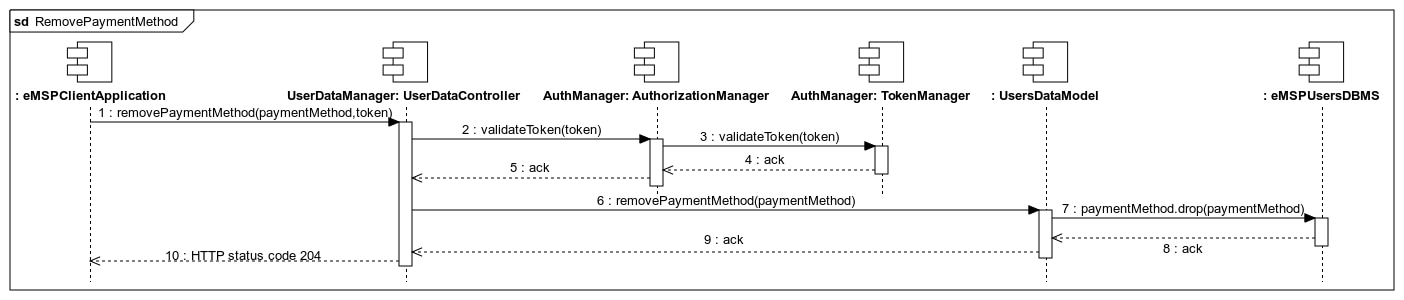
\includegraphics[width=1\textwidth]{Images/sequenceDiagrams/RemovePaymentMethod.jpg}
    \caption{Remove Payment Method}
\end{figure}
When a user wants to remove a payment method, the request is authorized through the token, and then the drop request is forwarded to the database.

\subsection{Make Reservation}
\begin{figure}[H]
    \centering
    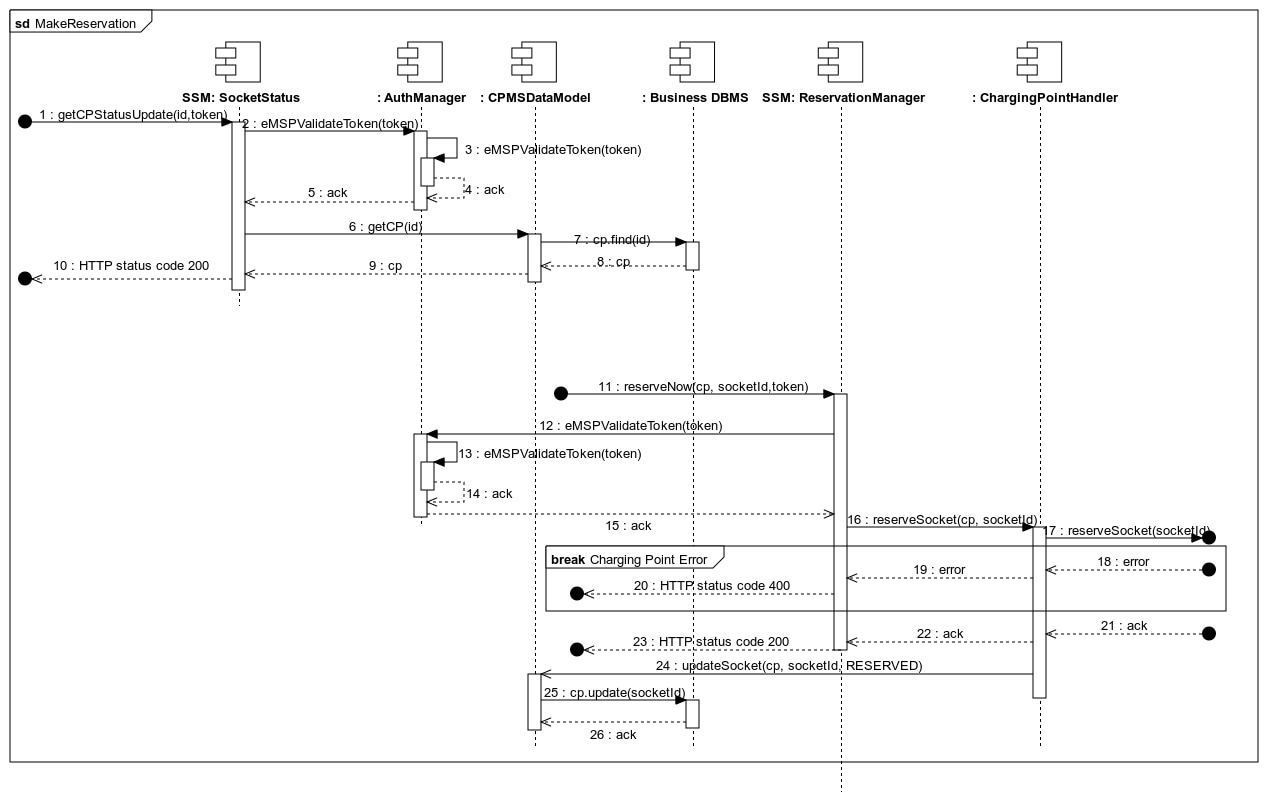
\includegraphics[width=1\textwidth]{Images/sequenceDiagrams/MakeReservation.jpg}
    \caption{Make Reservation on the eMSP side}
\end{figure}
When a user makes a reservation, first has to research for the CPs nearby a certain location. Once the system provides him the CPs saved in the local database (with the last status update received by the CPMSs), the user selects one of them and a request is sent to the CPMS to know the actual status of the CP with the relative sockets and send it to the user updating the local DB.
Once the user has all the information about the CP and the sockets, he sends a request for a reservation. A user is not able to reserve if has an active reservation or an old unpaid reservation. If he's valid the reserve request is forwarded to the CPMS related to that CP that will confirm or deny the reservation.

\begin{figure}[H]
    \centering
    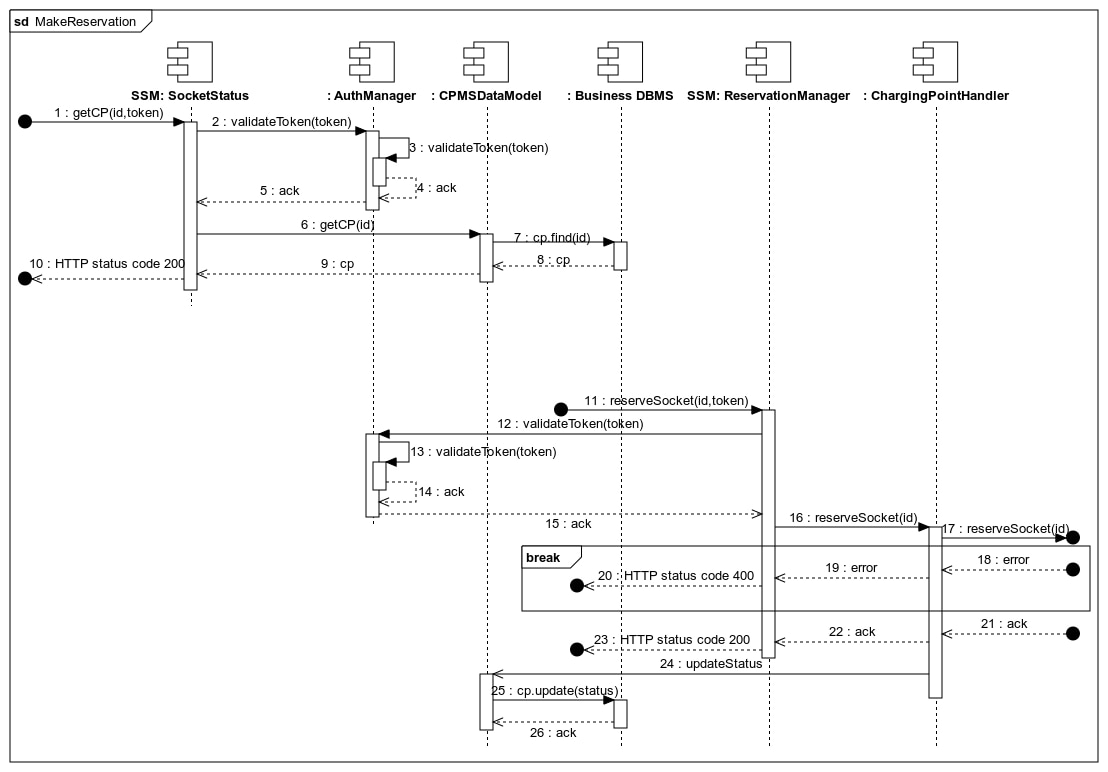
\includegraphics[width=1\textwidth]{Images/sequenceDiagrams/MakeReservation-CPMS.jpg}
    \caption{Make Reservation on the CPMS side}
\end{figure}
When the CPMS receives a request, first it validates the unique token provided by the eMSP that identifies it. Once authorized, a reservation request is forwarded to the CP using the OCPP protocol, and if no error occurs then the reservation is created, the eMSP is notified and the status update is sent to the internal database of the CPMS.


\subsection{Manage Charging Suggestion}
\begin{figure}[H]
    \centering
    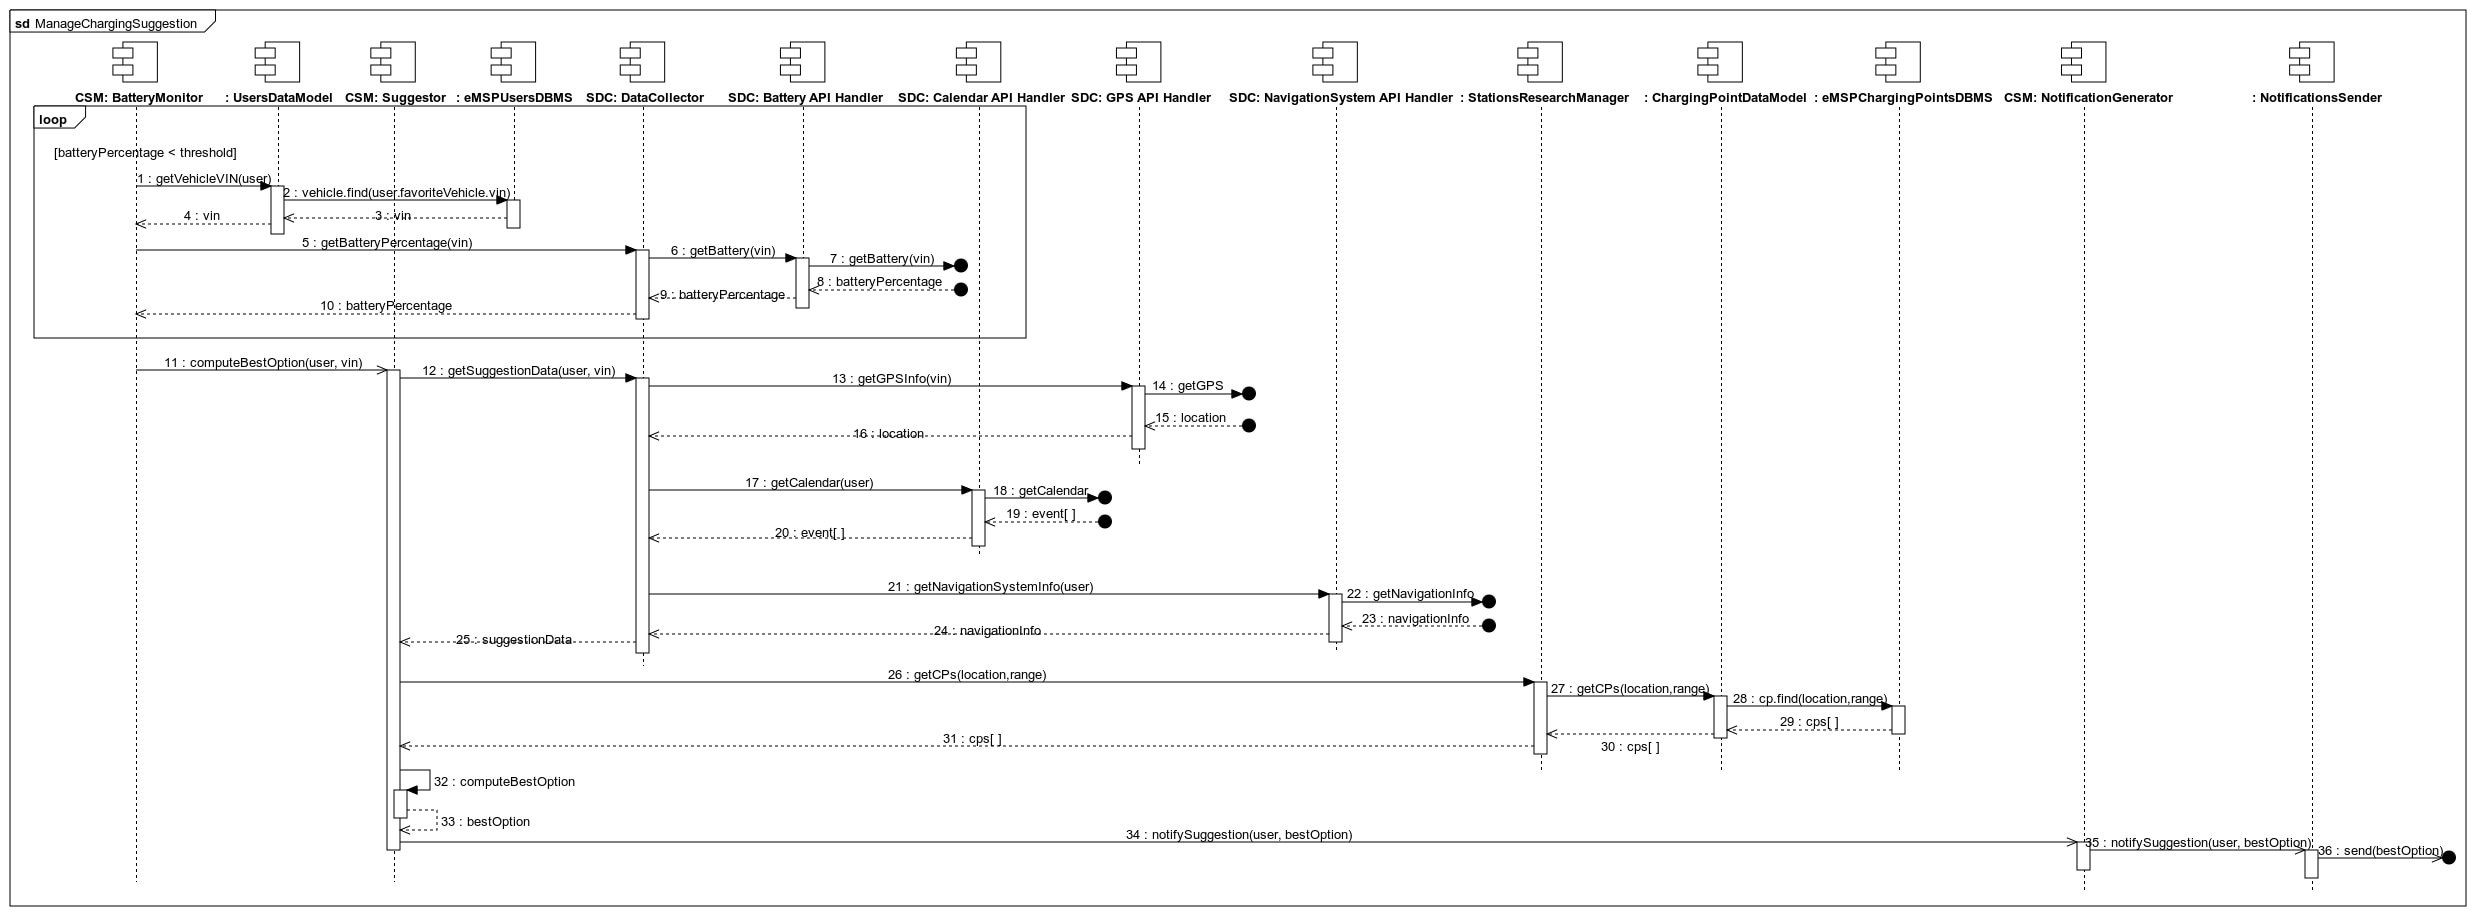
\includegraphics[width=1\textwidth]{Images/sequenceDiagrams/ManageChargingSuggestion.jpg}
    \caption{Manage Charging Suggestion}
\end{figure}
A charging suggestion is triggered when the battery of the vehicle, retrieved through the external API, is under a certain threshold. When this happens, the Suggestor component starts to retrieve all the data that it can access (calendar, GPS, and/or Navigation System) through external APIs. Once all data are collected, the Suggestor searches the CPs near a spot it estimates the best and selects one socket compatible with the vehicle. Then the proposal is sent through a notification to the user that can refuse it or start the reservation process to that socket.

\subsection{Cancel Reservation}
\begin{figure}[H]
    \centering
    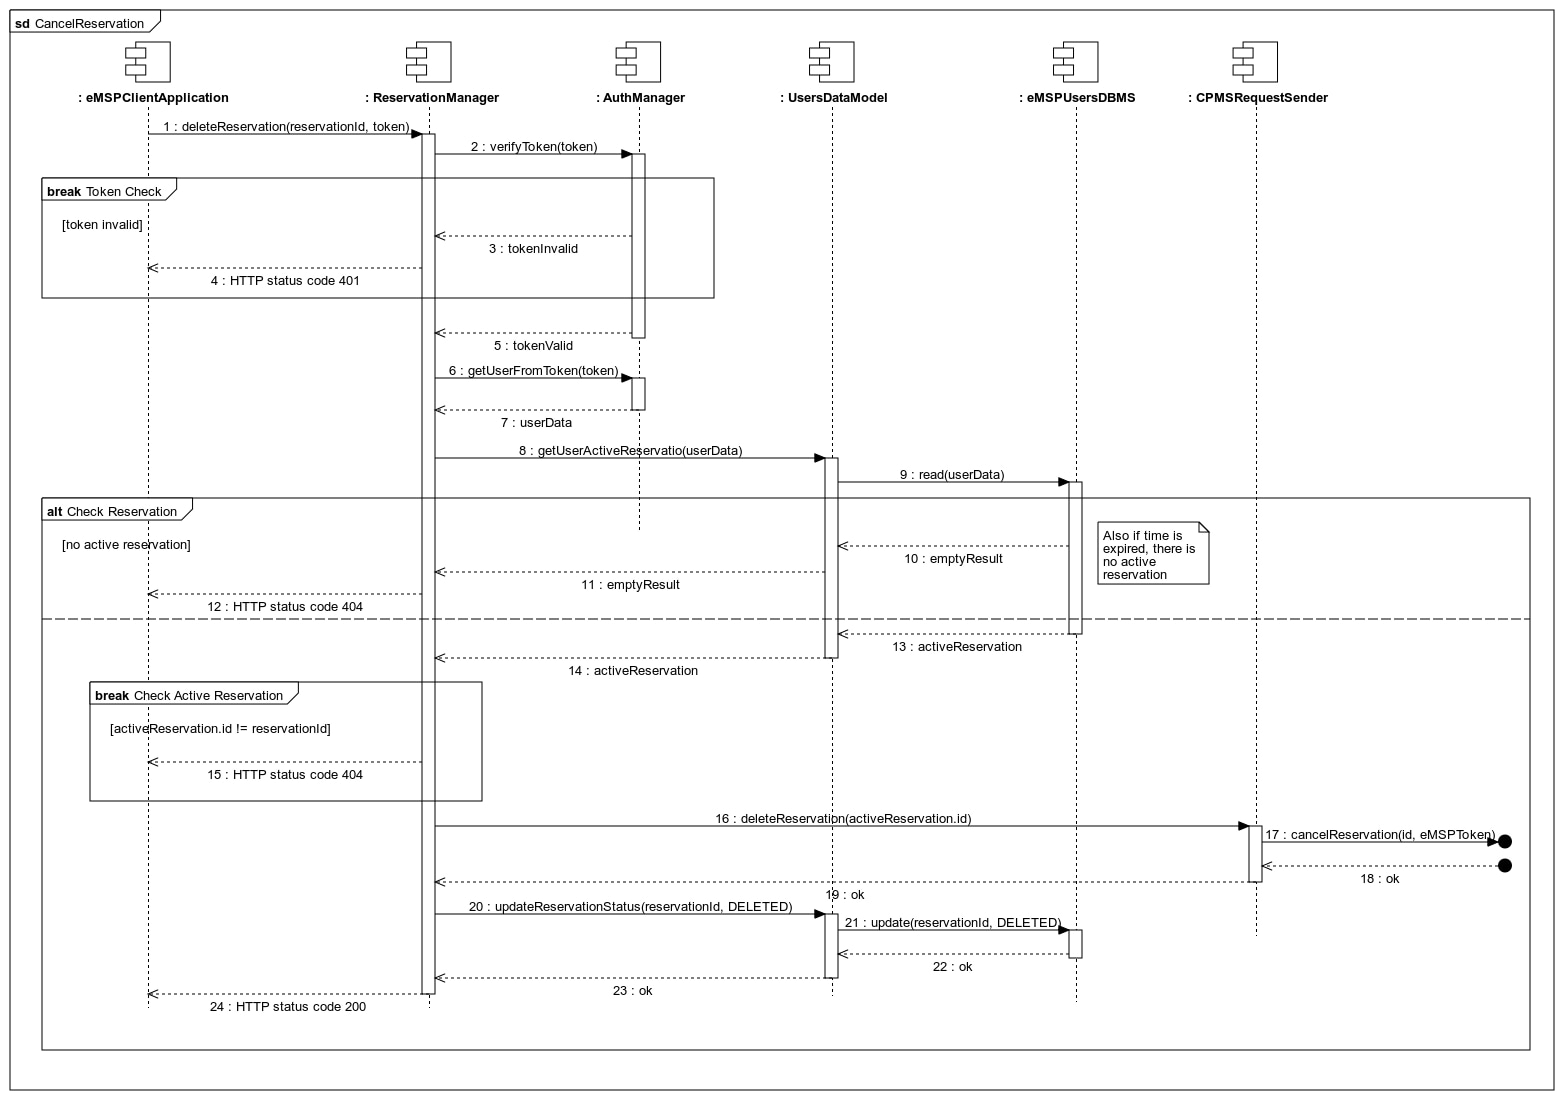
\includegraphics[width=1\textwidth]{Images/sequenceDiagrams/CancelReservation.jpg}
    \caption{Cancel Reservation on the eMSP side}
\end{figure}
After verifying the token validity and retrieving the user by it, the system gets his active reservation from the DB. If the active reservation is found and corresponds to the provided reservation, then the cancellation request is forwarded to the related CPMS;
after a positive response, the new status of the reservation is saved in the DB.

\begin{figure}[H]
    \centering
    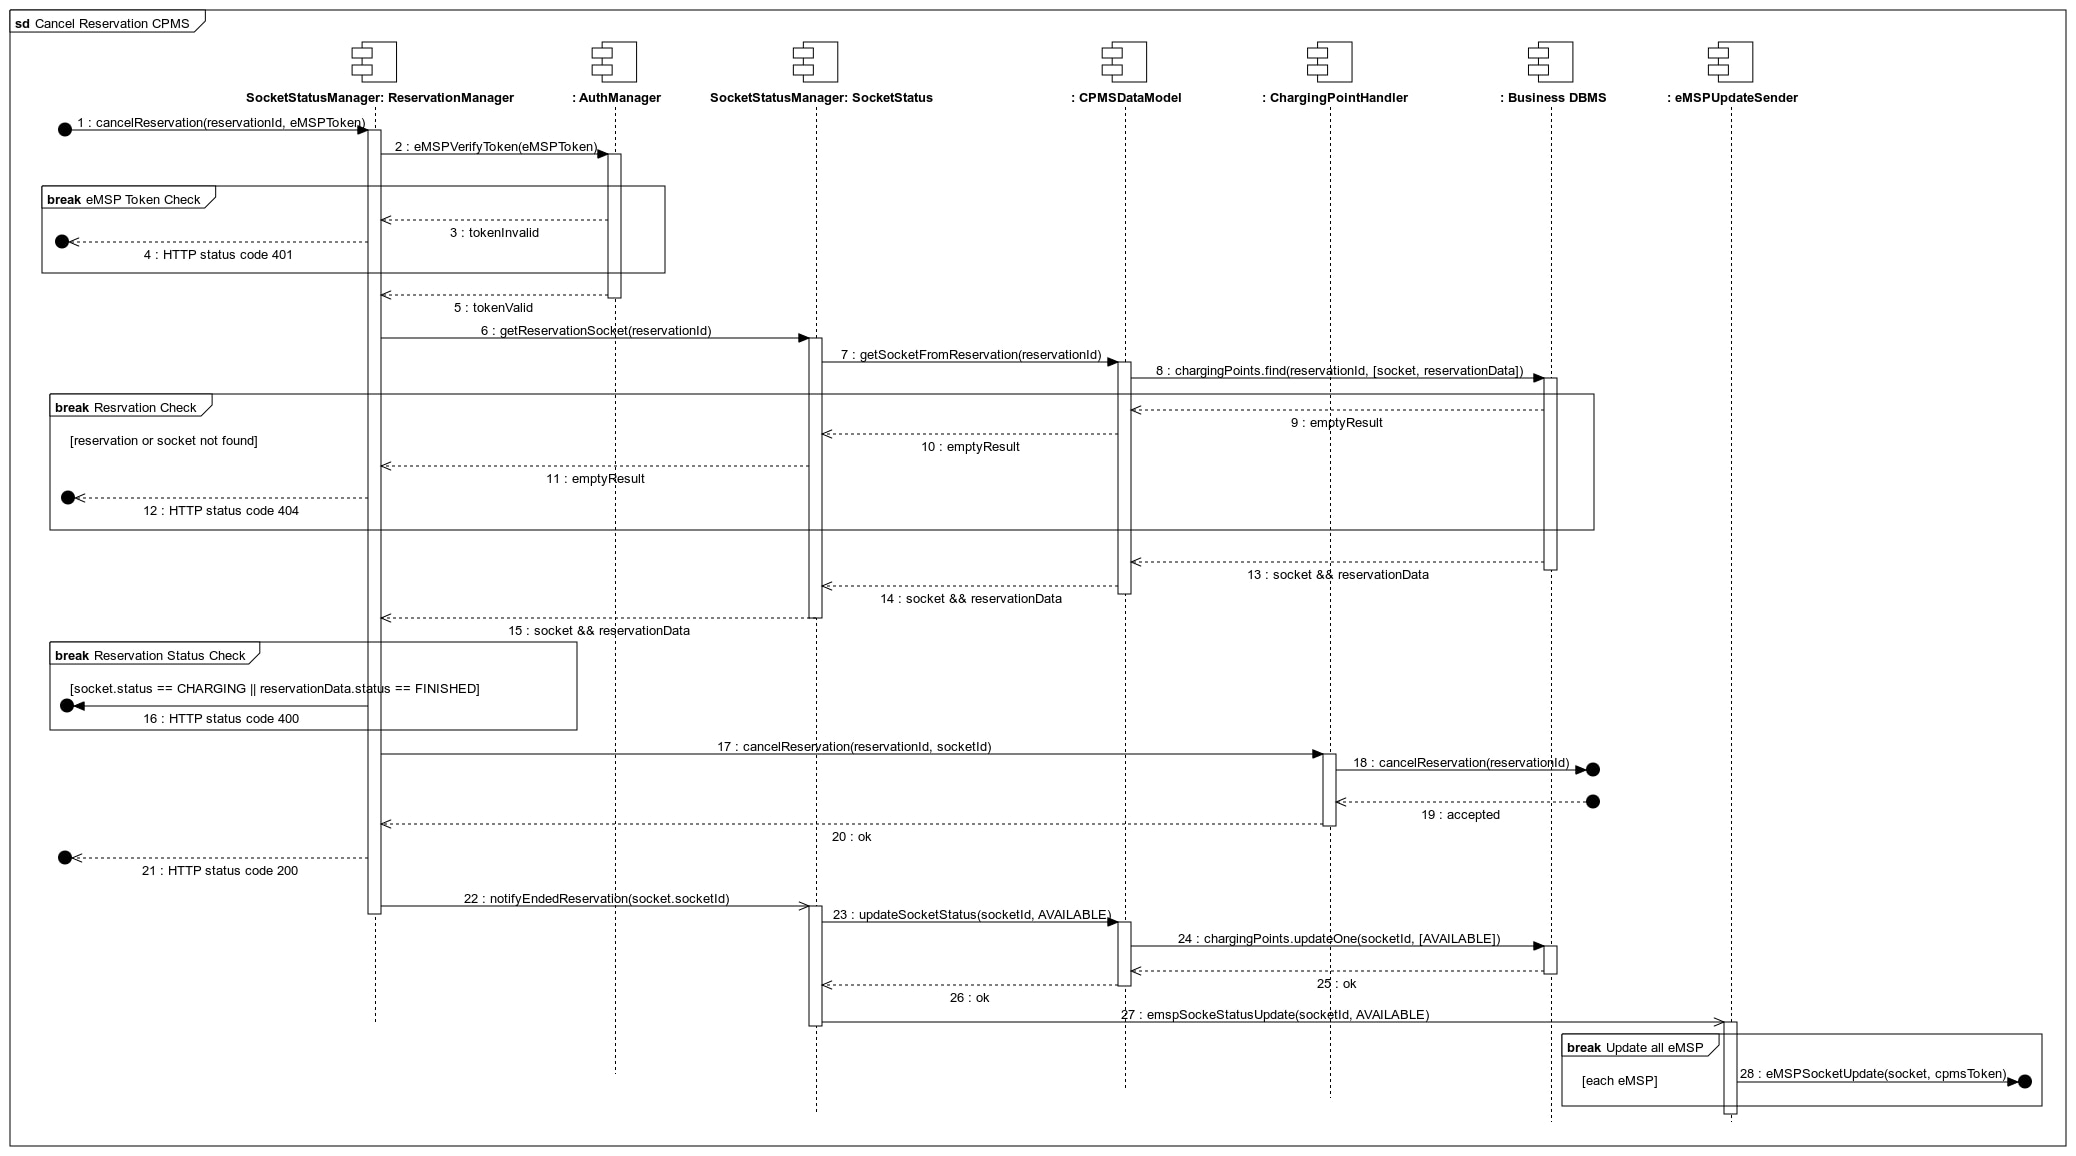
\includegraphics[width=1\textwidth]{Images/sequenceDiagrams/Cancel Reservation CPMS.jpg}
    \caption{Cancel Reservation on the CPMS side}
\end{figure}
When the CPMS Server receives a cancel reservation, it validates the request through the token provided by an eMSP, and if valid, it retrieves the socket related to the reservation. Once a reservation is found its status has to be verified, if the charging session is either started or finished, it cannot be deleted, otherwise the request is forwarded to the socket.
Once the reservation is deleted the response is sent to the eMSP that made the request at the beginning and the new socket status is saved on the database and notified to every eMSP connected to the CPMS.

\subsection{Start Charging Process}
\begin{figure}[H]
    \centering
    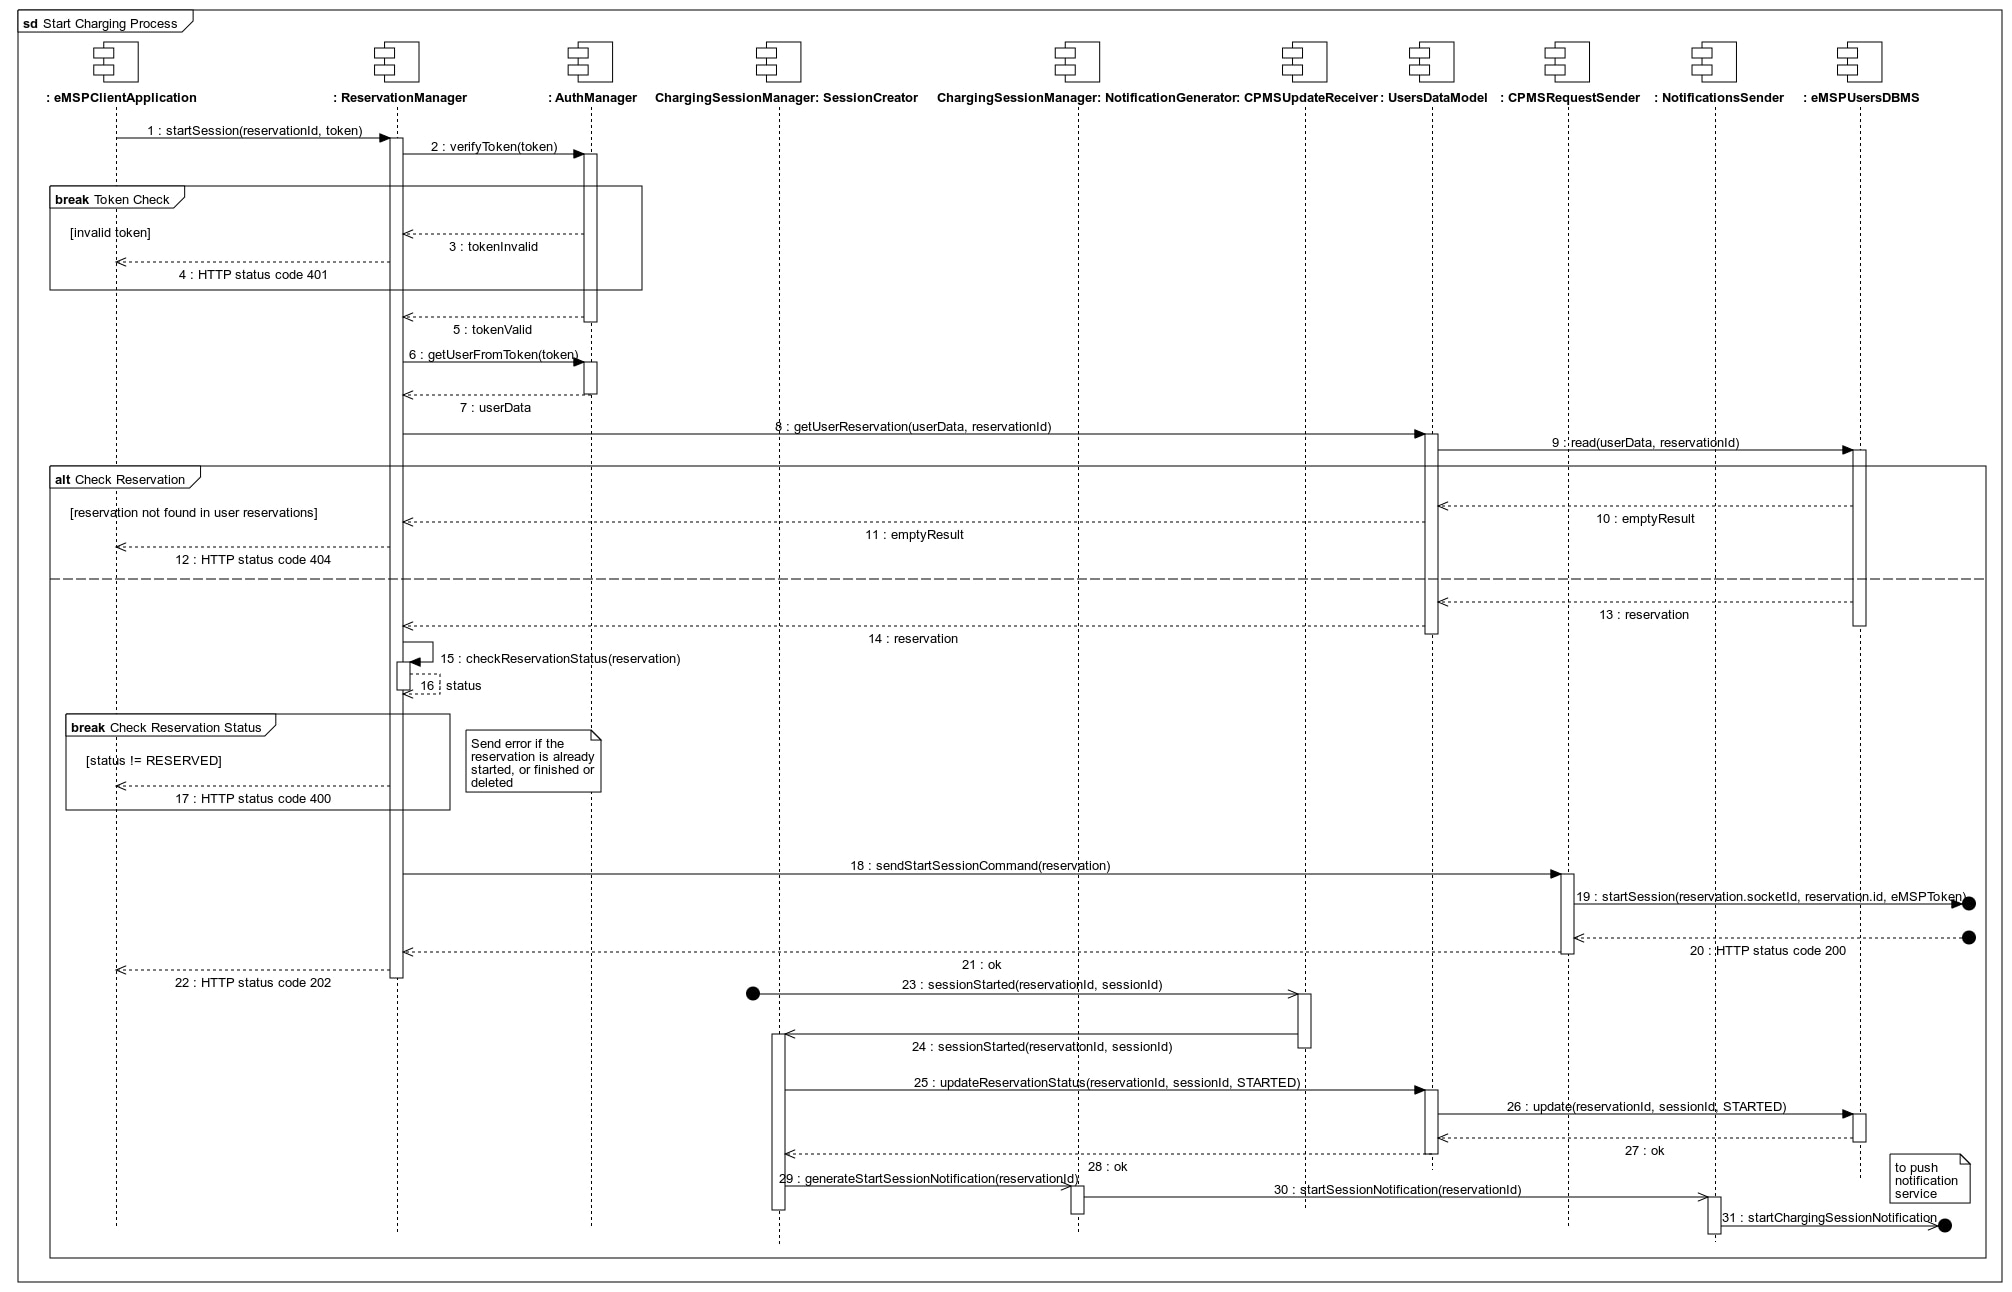
\includegraphics[width=1\textwidth]{Images/sequenceDiagrams/Start Charging Process.jpg}
    \caption{Start Charging Process on the eMSP side}
\end{figure}
A charging session can be started by the user if and only if a reservation is made before. After verifying the validity of the token provided by the client, the reservation is retrieved from the database, if the status isn't reserved returns an error otherwise the start charging session request is sent to the CPMS that takes over the request letting know the user now he can plug the socket into the vehicle. Once the Charging Point starts the energy flow, the CPMS sends a message to the eMSP that updates the status of the reservation; then, the eMSP notifies the user through the push notification service.

\begin{figure}[H]
    \centering
    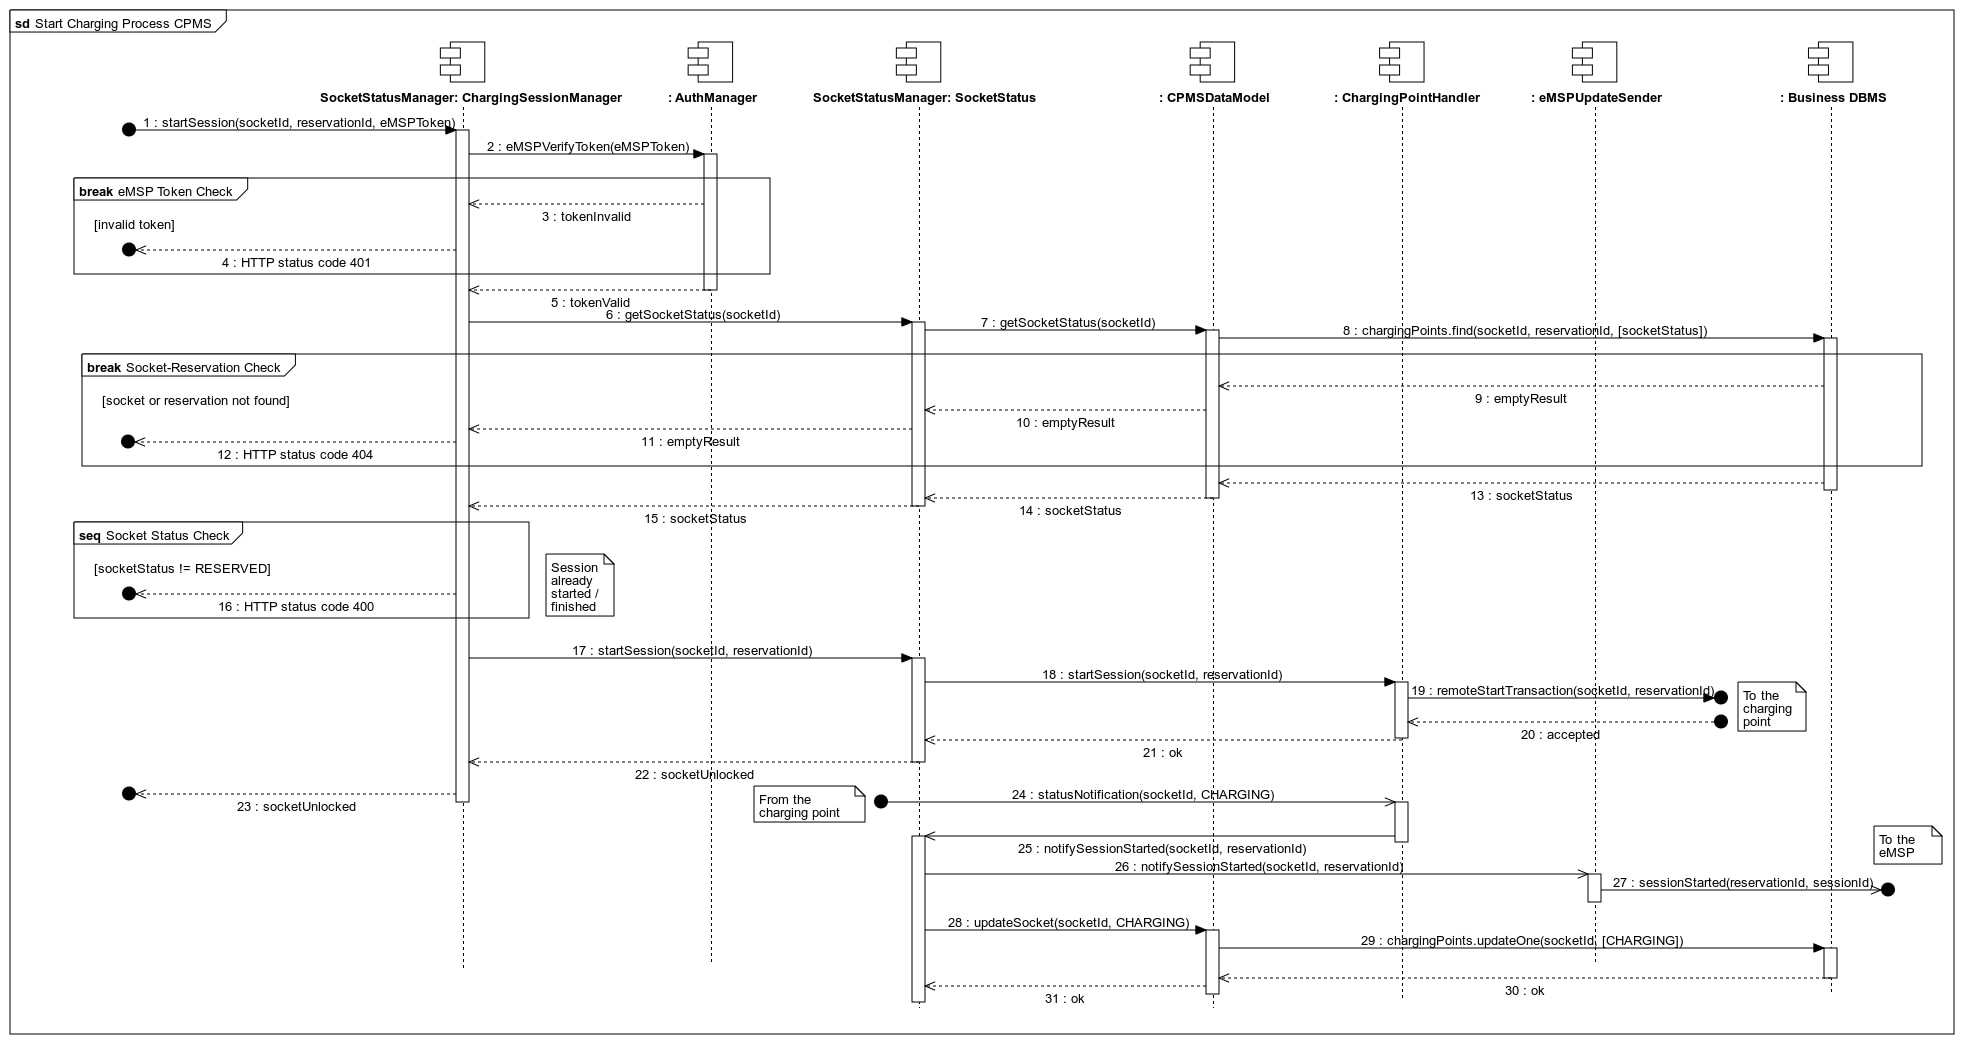
\includegraphics[width=1\textwidth]{Images/sequenceDiagrams/Start Charging Process CPMS.jpg}
    \caption{Start Charging Process on the CPMS side}
\end{figure}
The CPMS receiving the start session request verifies the validity of the token, the existence, and the status of the socket and then forwards the request to that socket.
Once the socket accepts the request, unlocks itself and sends back the response to the server that notifies the eMSP that made the call. Once the charging point recognizes the plugged socket and starts the energy flow, it notifies the CPMS which updates the status in the DB and, in turn, notifies the eMSP.

\subsection{End Charging Process}
\begin{figure}[H]
    \centering
    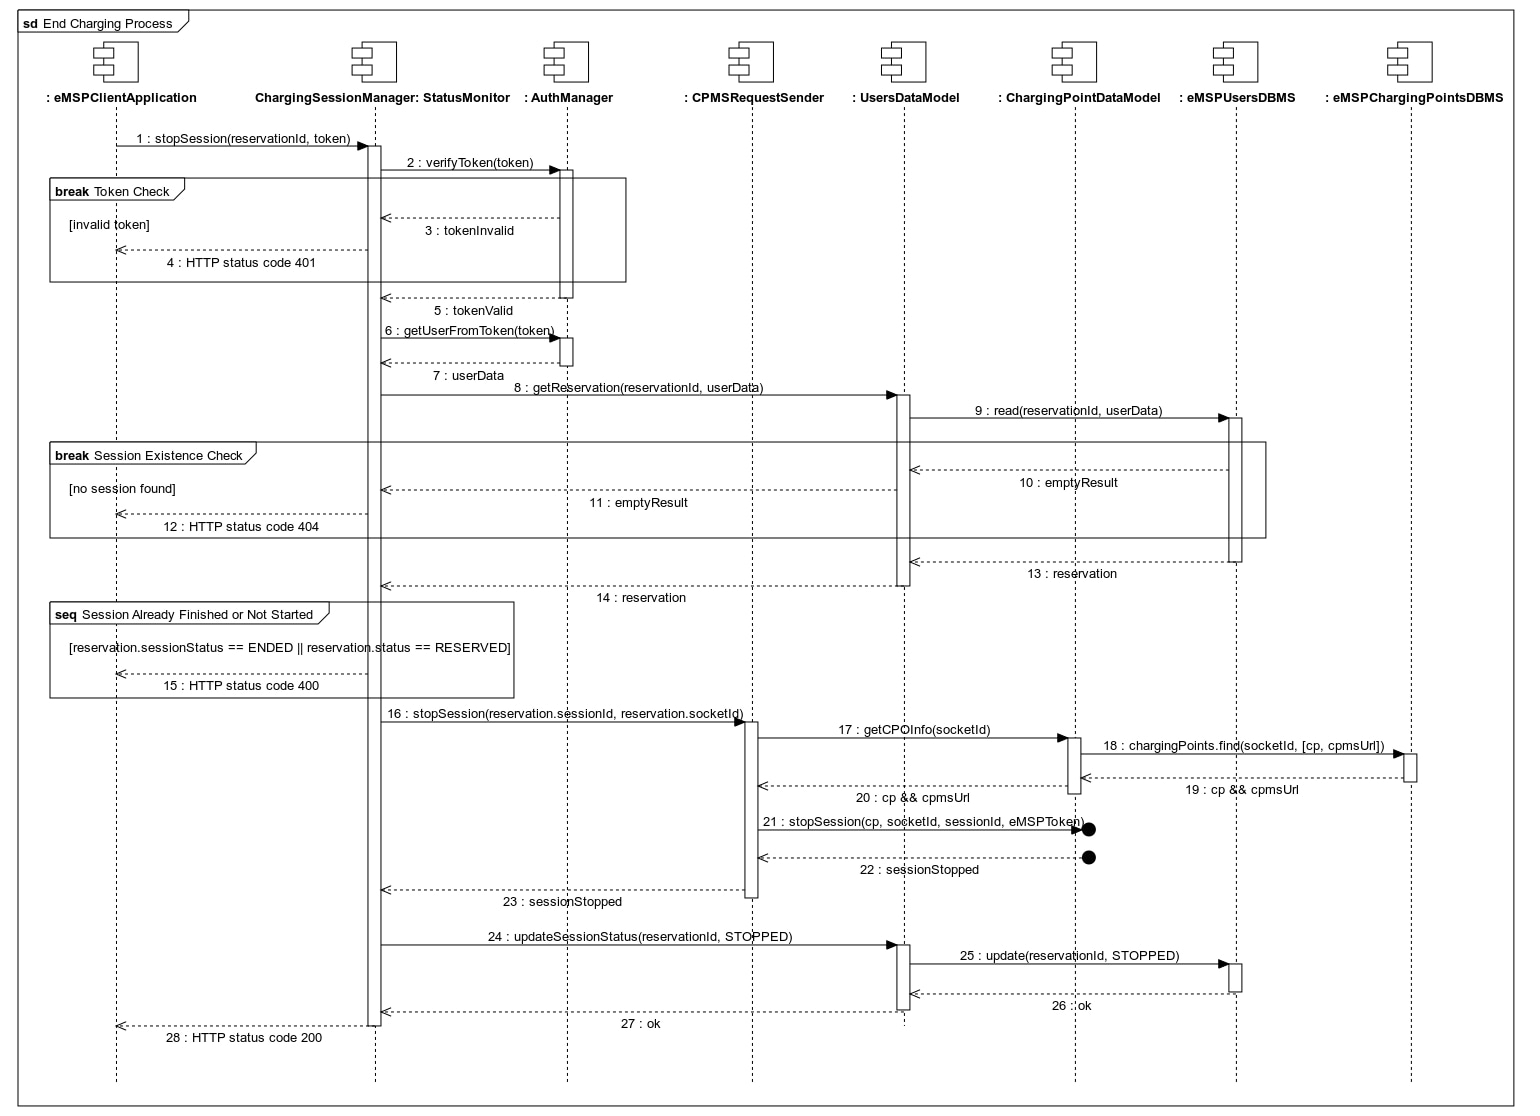
\includegraphics[width=1\textwidth]{Images/sequenceDiagrams/End Charging Process.jpg}
    \caption{End Charging Process on the eMSP side}
\end{figure}
After all the usual verifications of the token and the reservation, the system retrieves all the information in order to know to which CPMS send the stop session request. Once the request is sent and a confirmation is returned, the server updates its database with the new status of the charging session.

\begin{figure}[H]
    \centering
    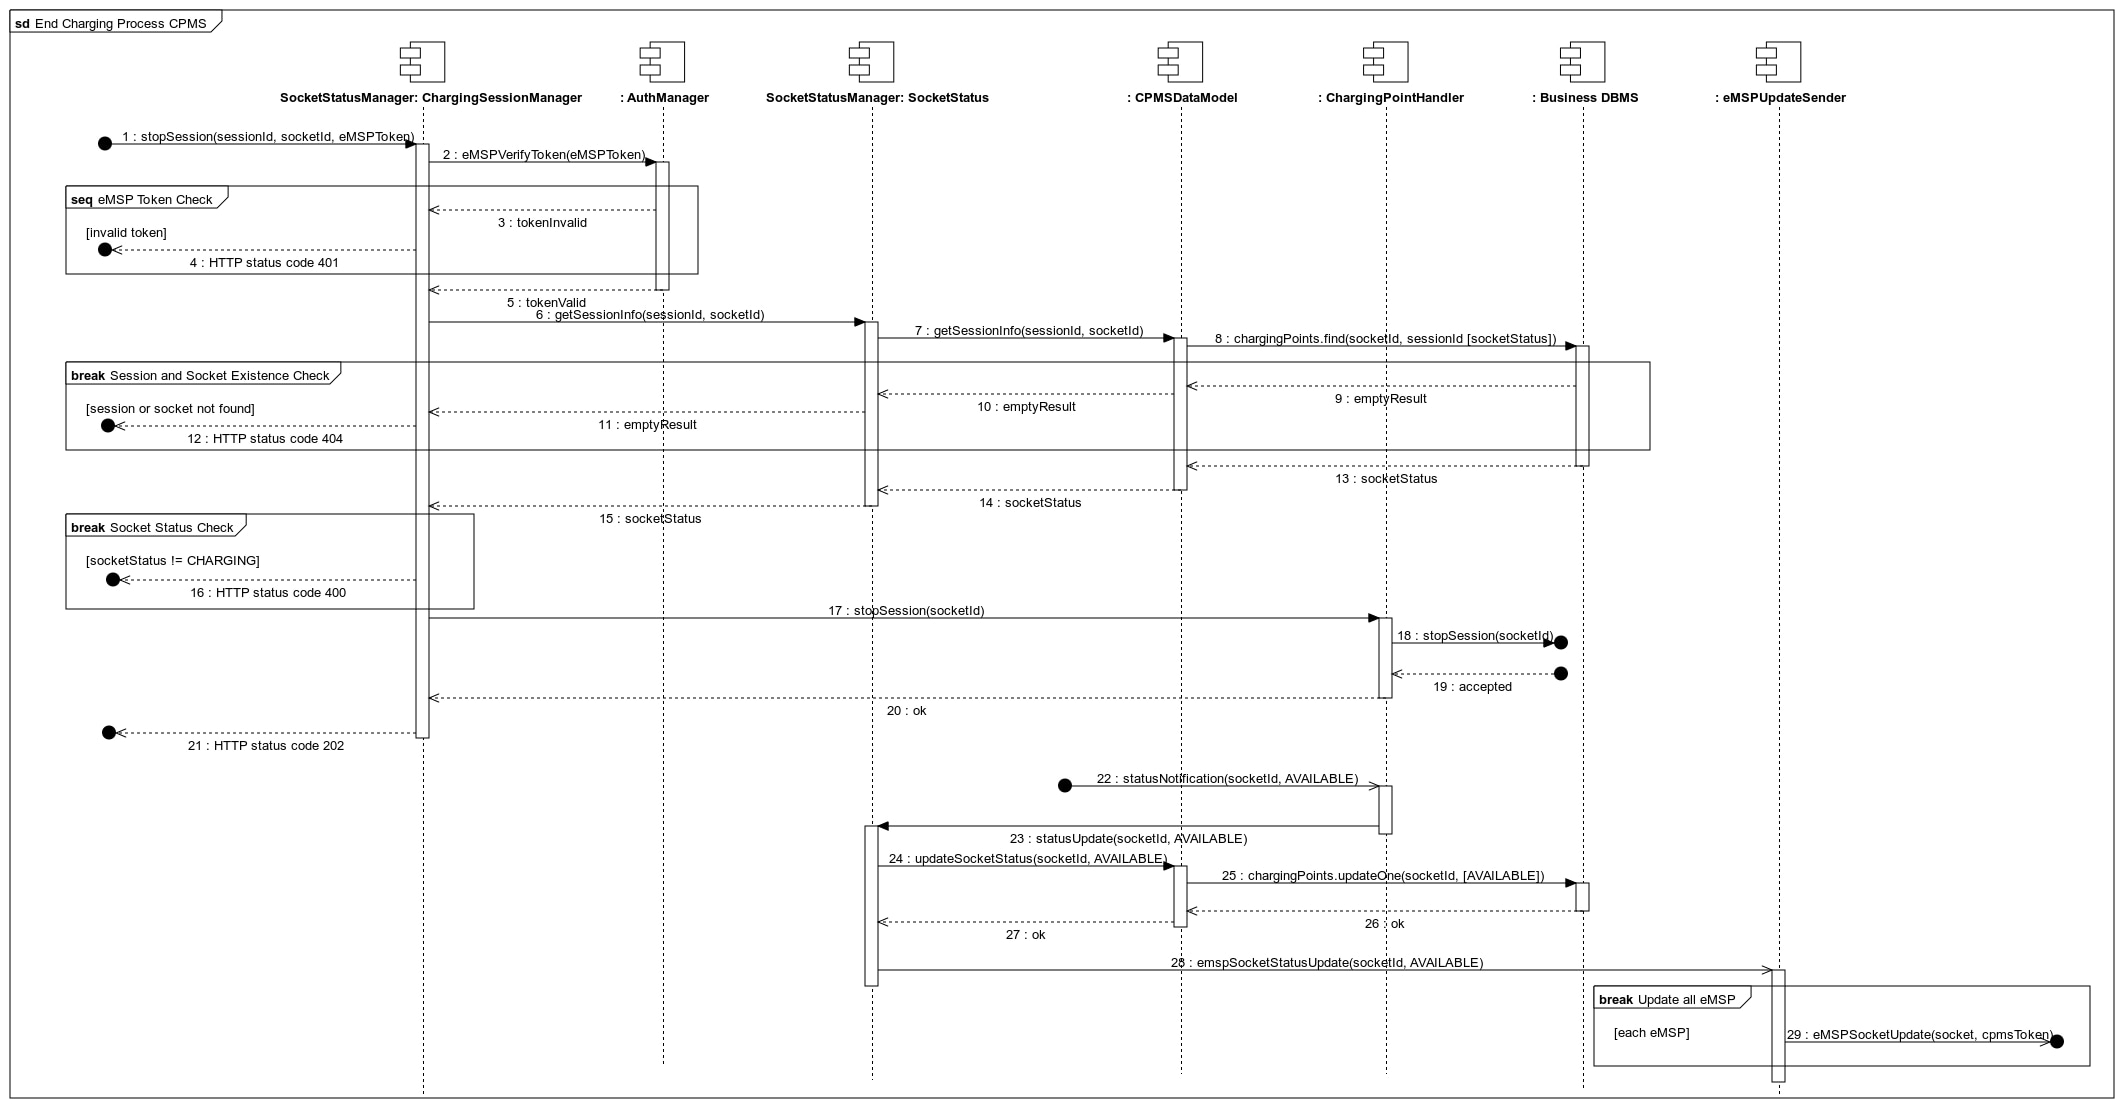
\includegraphics[width=1\textwidth]{Images/sequenceDiagrams/End Charging Process CPMS.jpg}
    \caption{End Charging Process on the CPMS side}
\end{figure}
On the CPMS side, once all verifications have been made, the stop session is sent to the CP that responds to it with a confirmation message which in turn is sent to eMSP.
The CP notifies the CPMS once its status returns available (i.e. once the user unplugs the socket). The CPMS will then update all the eMSPs connected to it.

\subsection{Pay Session}
\begin{figure}[H]
    \centering
    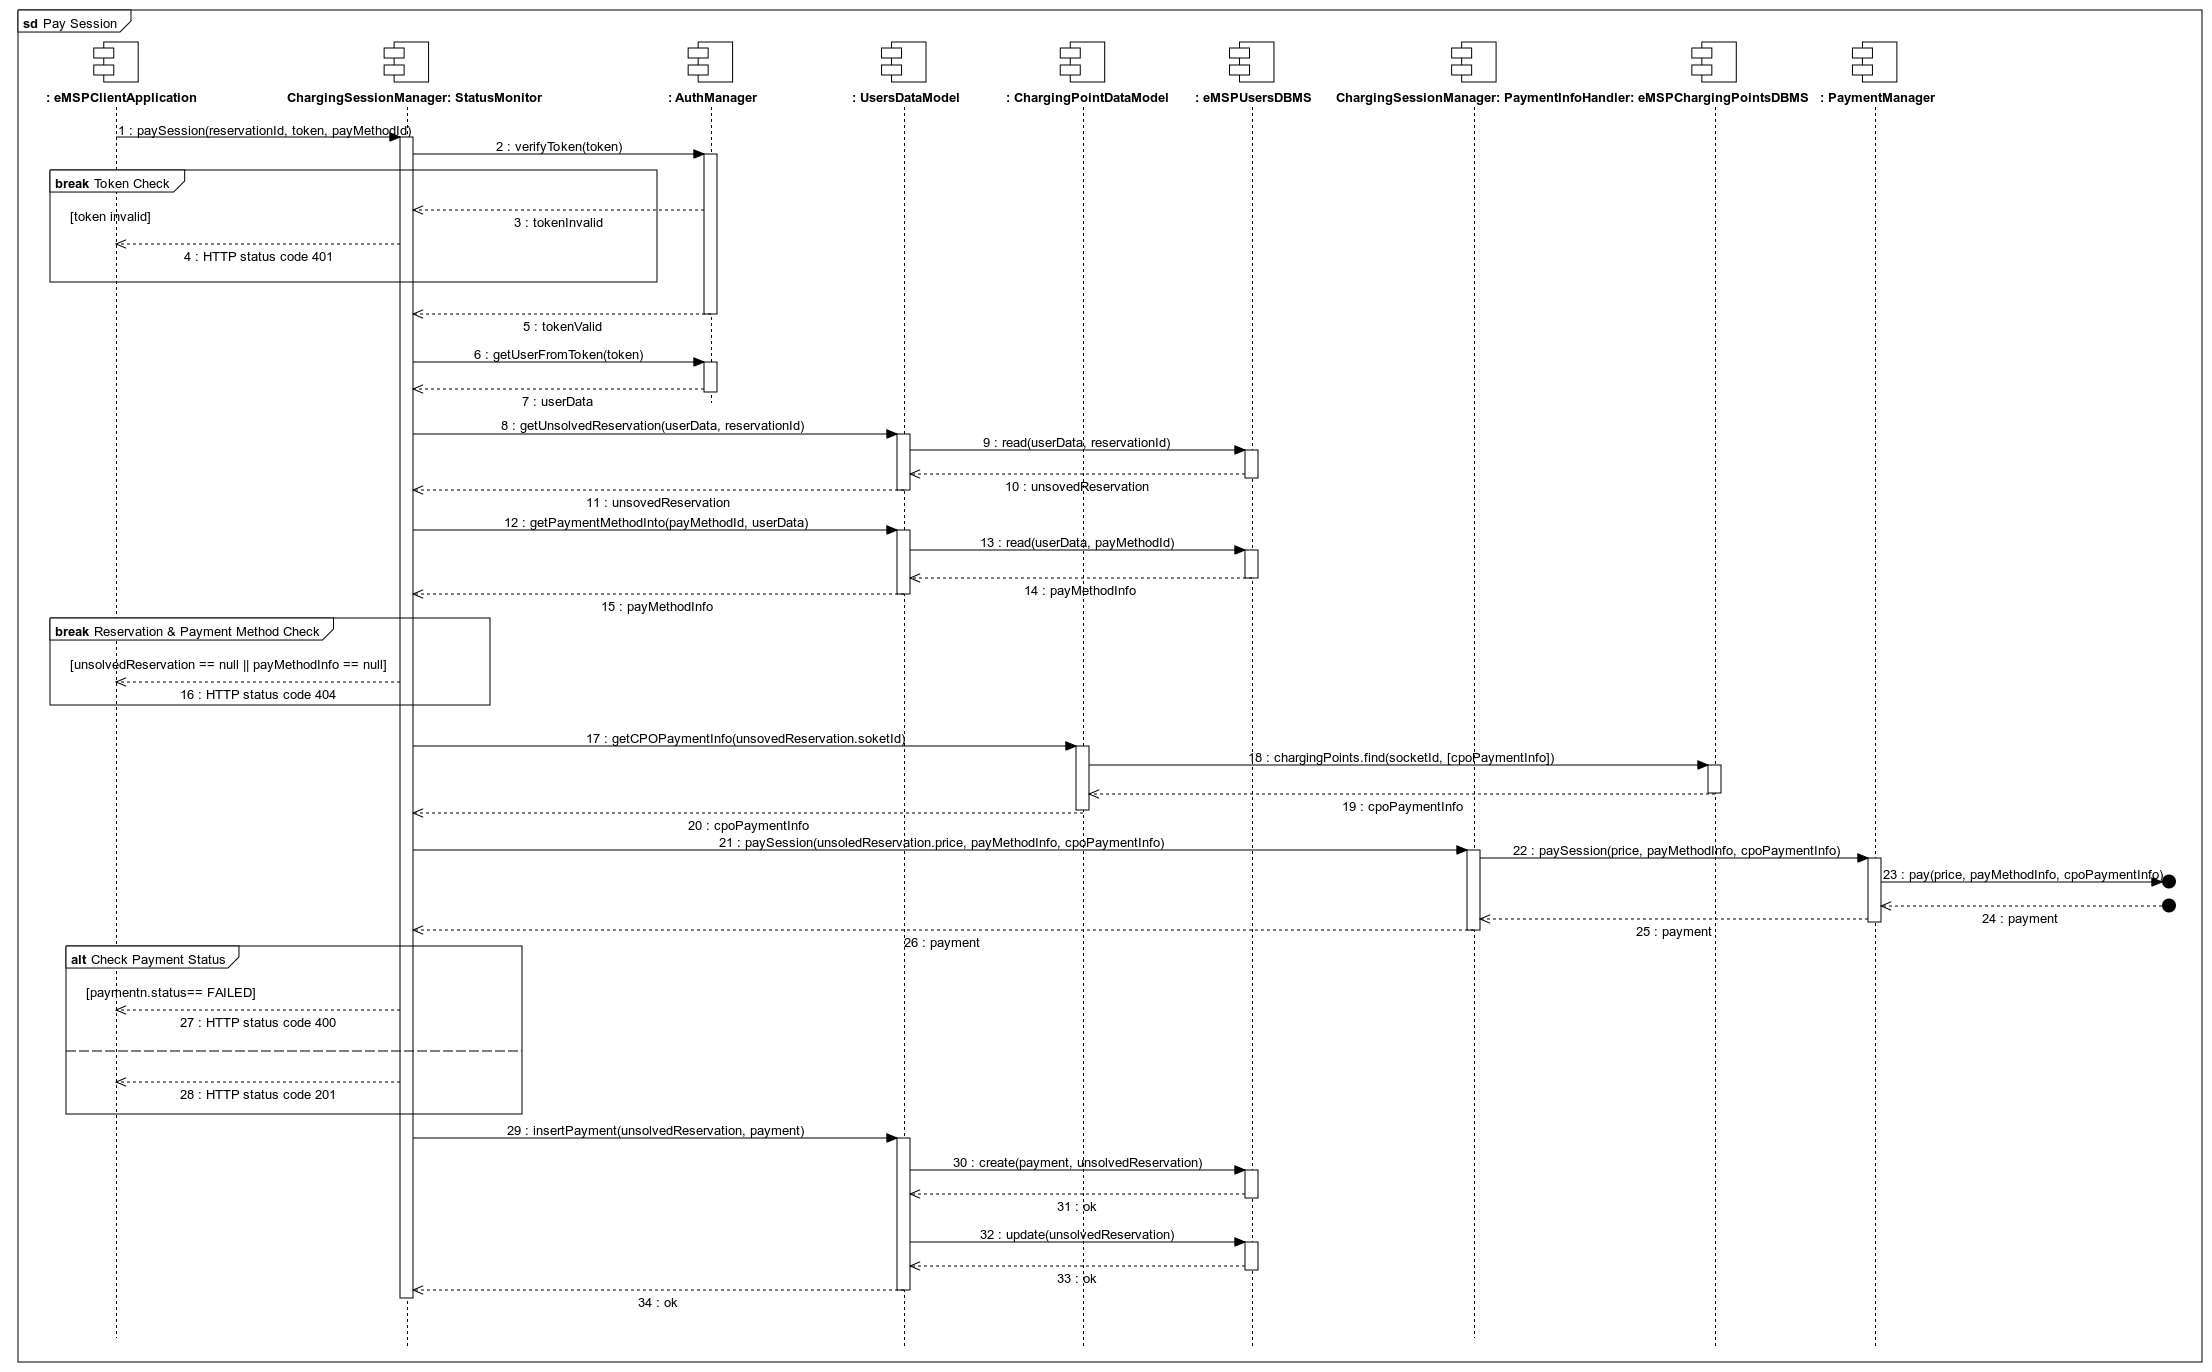
\includegraphics[width=1\textwidth]{Images/sequenceDiagrams/Pay Session.jpg}
    \caption{Pay Session}
\end{figure}
Before paying for a session the system checks if there exists actually an unpaid reservation and gets the user payment method. If both conditions are satisfied the system retrieves the payment coordinates of the CPMS related to the socket of the reservation. With all this information and the amount to pay, an external API takes care of the payment giving back the result of the payment. No matter what the outcome is, the payment is saved and the status of the reservation is updated in the DB, but different messages are sent to the client.

\subsection{CPO Registration}
\begin{figure}[H]
    \centering
    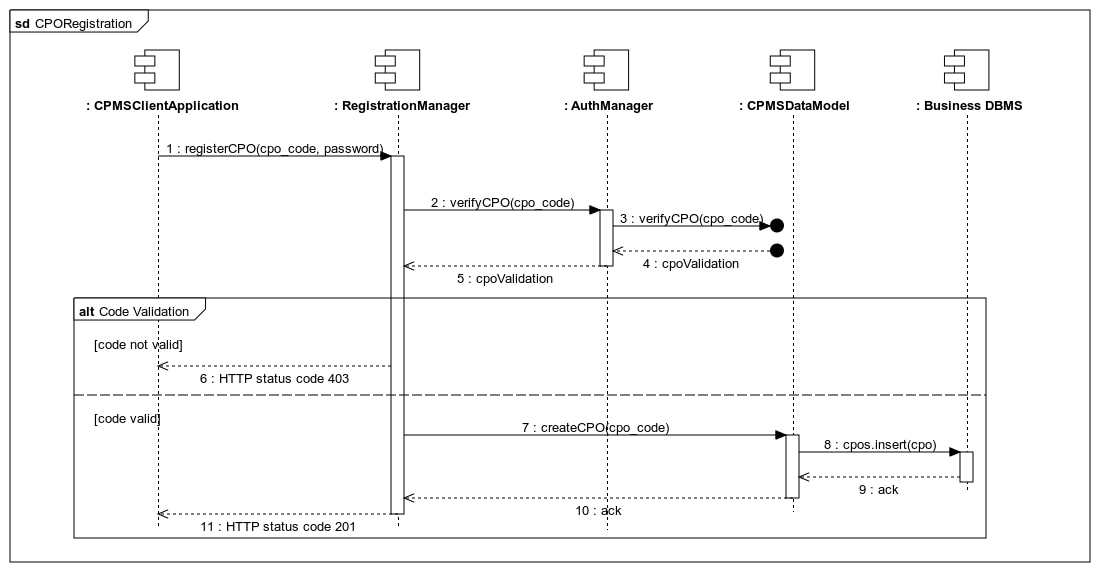
\includegraphics[width=1\textwidth]{Images/sequenceDiagrams/CPORegistration.jpg}
    \caption{CPO Registration}
\end{figure}

When a CPO wants to register to the CPMS, has to compile a form with his unique code (provided by external entities) and a password used as credentials. An external API takes care of verifying that the code is correct, if so the CPO credentials are saved in the system, otherwise, an error is sent to the client.

\subsection{CPO Login}
\begin{figure}[H]
    \centering
    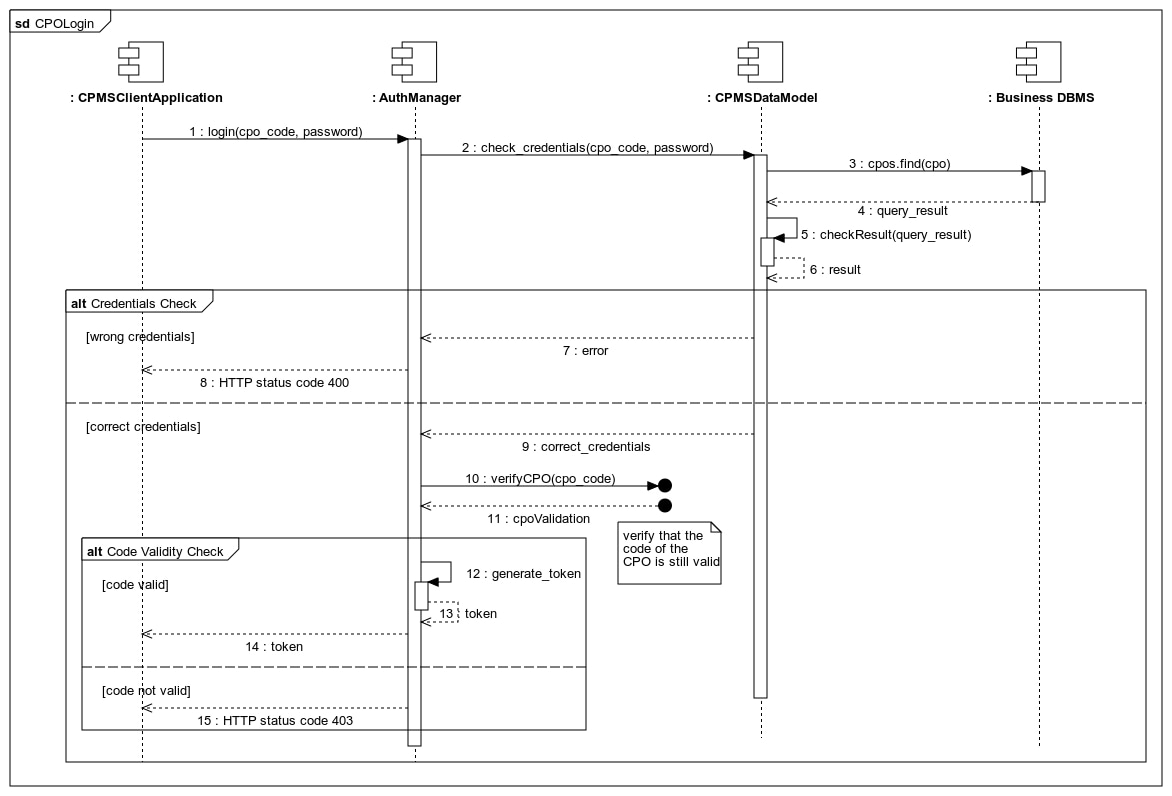
\includegraphics[width=1\textwidth]{Images/sequenceDiagrams/CPOLogin.jpg}
    \caption{CPO Login}
\end{figure}

In order to log in to the CPMS, a login request containing the code of the CPO and the password is sent to the Auth Manager. The Auth Manager first checks if there exists such a CPO in the system, if not an error is sent to the client. Then it checks if the code of the CPO is still valid (in order to detect, for example, if the CPO is no anymore habilitated as a CPO). If the code is not valid an error is sent to the client. Otherwise, a token is generated for the CPO that will use it for other requests.

\subsection{Add CP}
\begin{figure}[H]
    \centering
    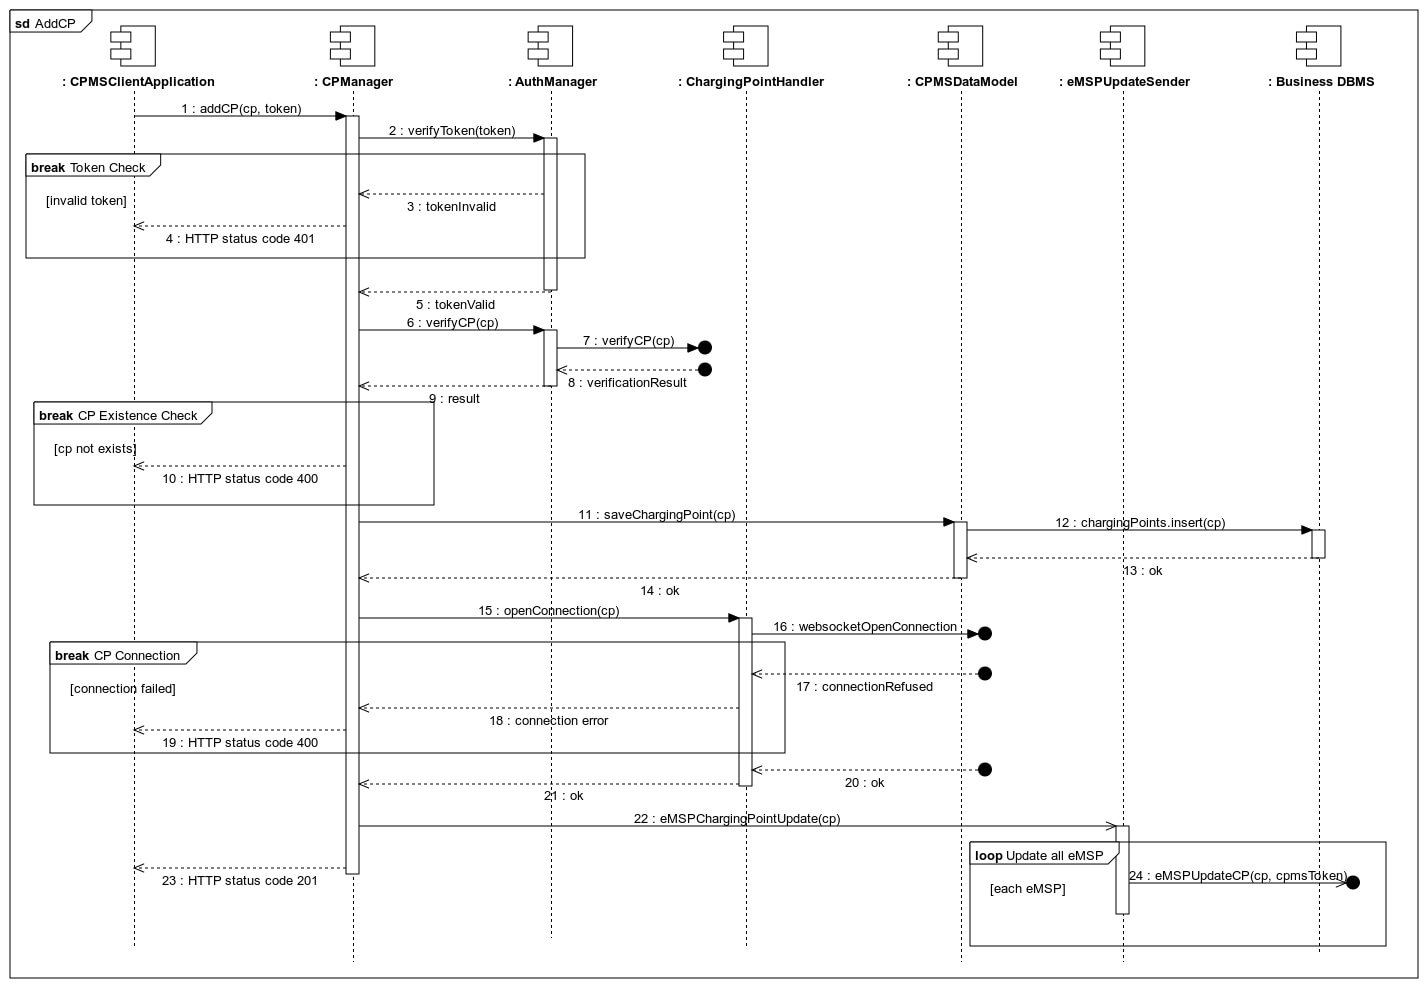
\includegraphics[width=1\textwidth]{Images/sequenceDiagrams/AddCP.jpg}
    \caption{Add CP}
\end{figure}
Adding a CP is verified through an external API, if the response is positive, the CP and the relative sockets are saved into the database. Once the CP is added the CPMS server tries to establish a connection to it, once the connection is established the server notifies all the CP information to the connected eMSPs.

\subsection{Manage CP's Battery Energy Flow}
\begin{figure}[H]
    \centering
    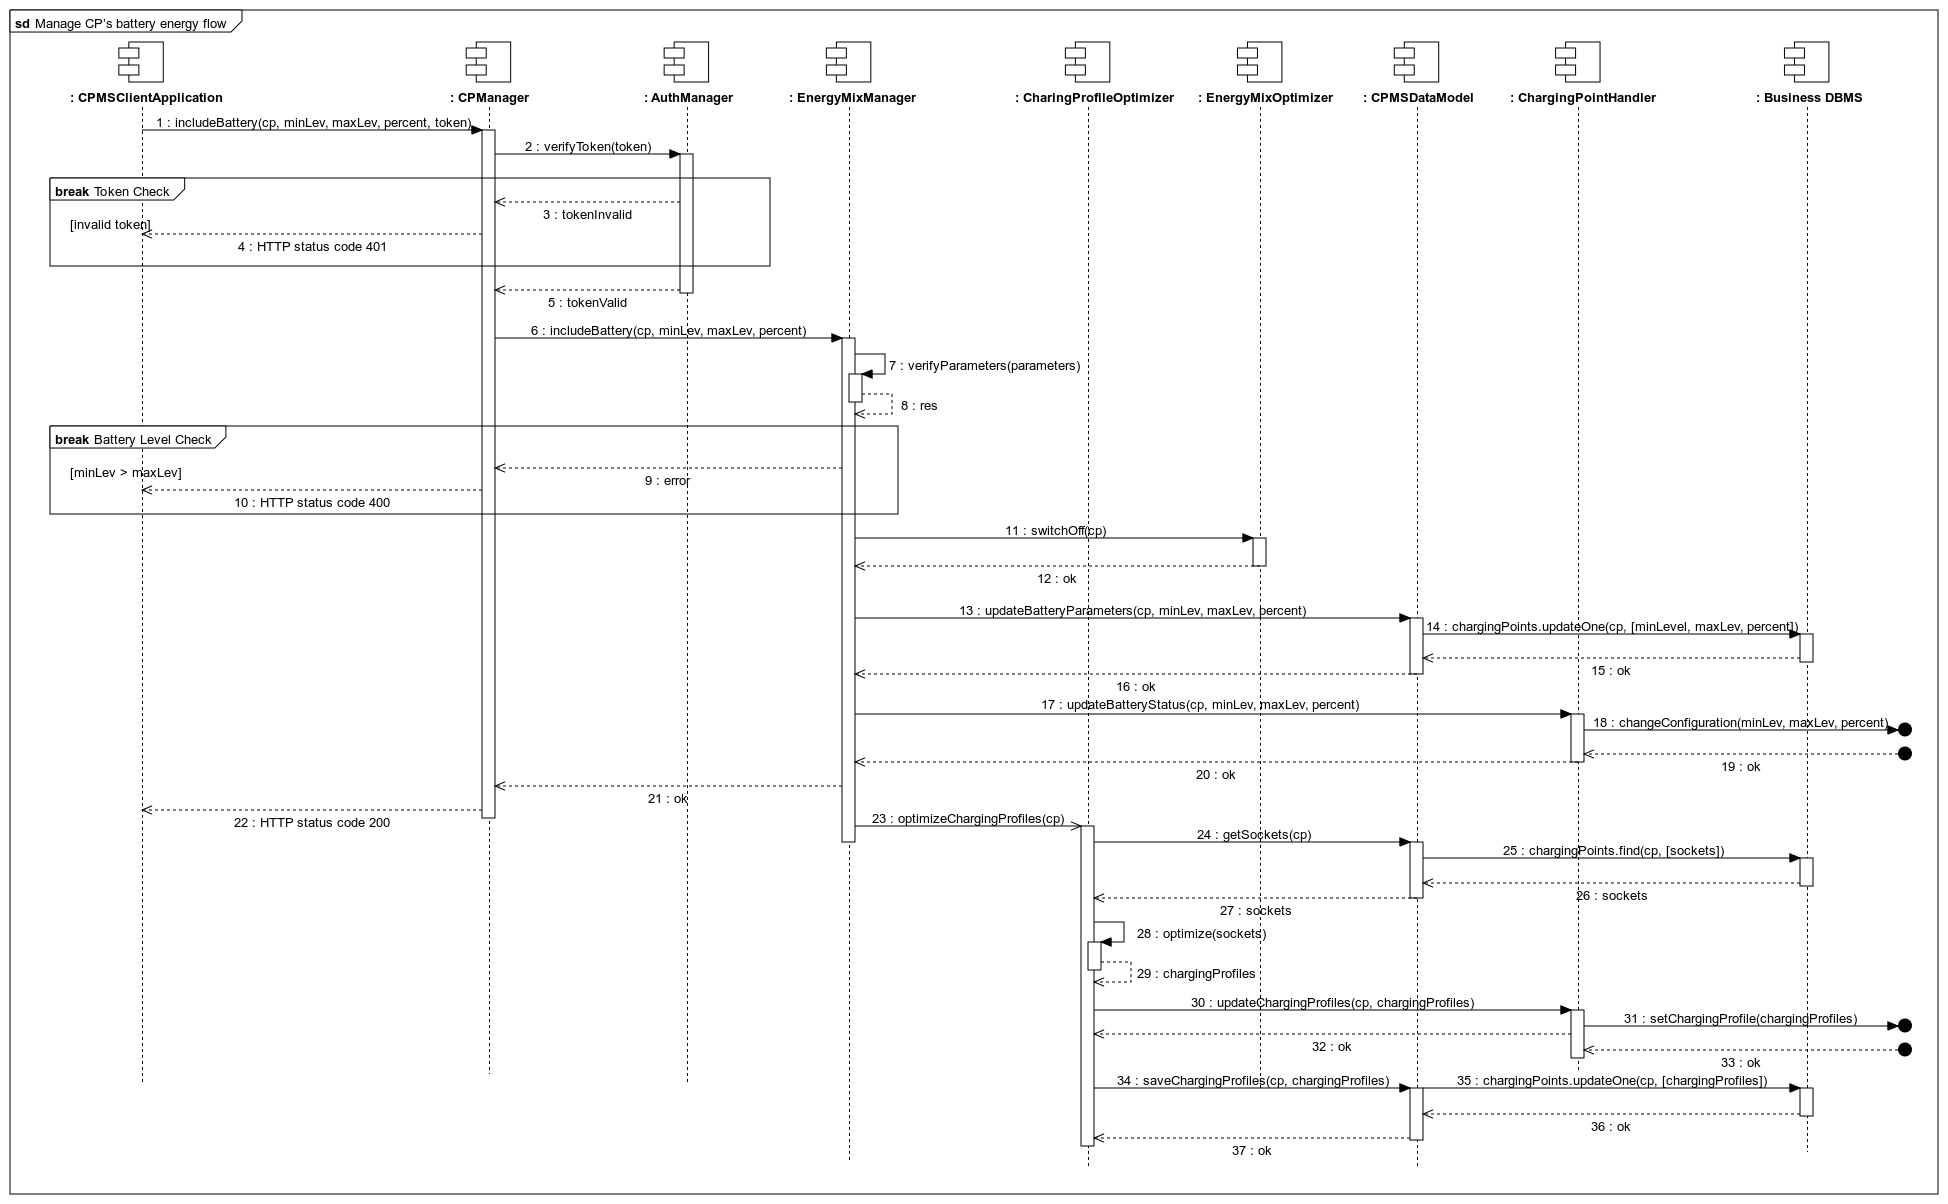
\includegraphics[width=1\textwidth]{Images/sequenceDiagrams/Manage CP battery energy flow.jpg}
    \caption{Manage CP's Battery Energy Flow}
\end{figure}
When a CPO manually enables the battery management, overwrites the values of the Energy Optimizer that is automatically switched off. The new settings are then saved in the local DB and sent to the CP. Once all is set a response is sent to the client and the optimization of the charging profiles is done in the background.

\subsection{Change Socket Availabilty}
\begin{figure}[H]
    \centering
    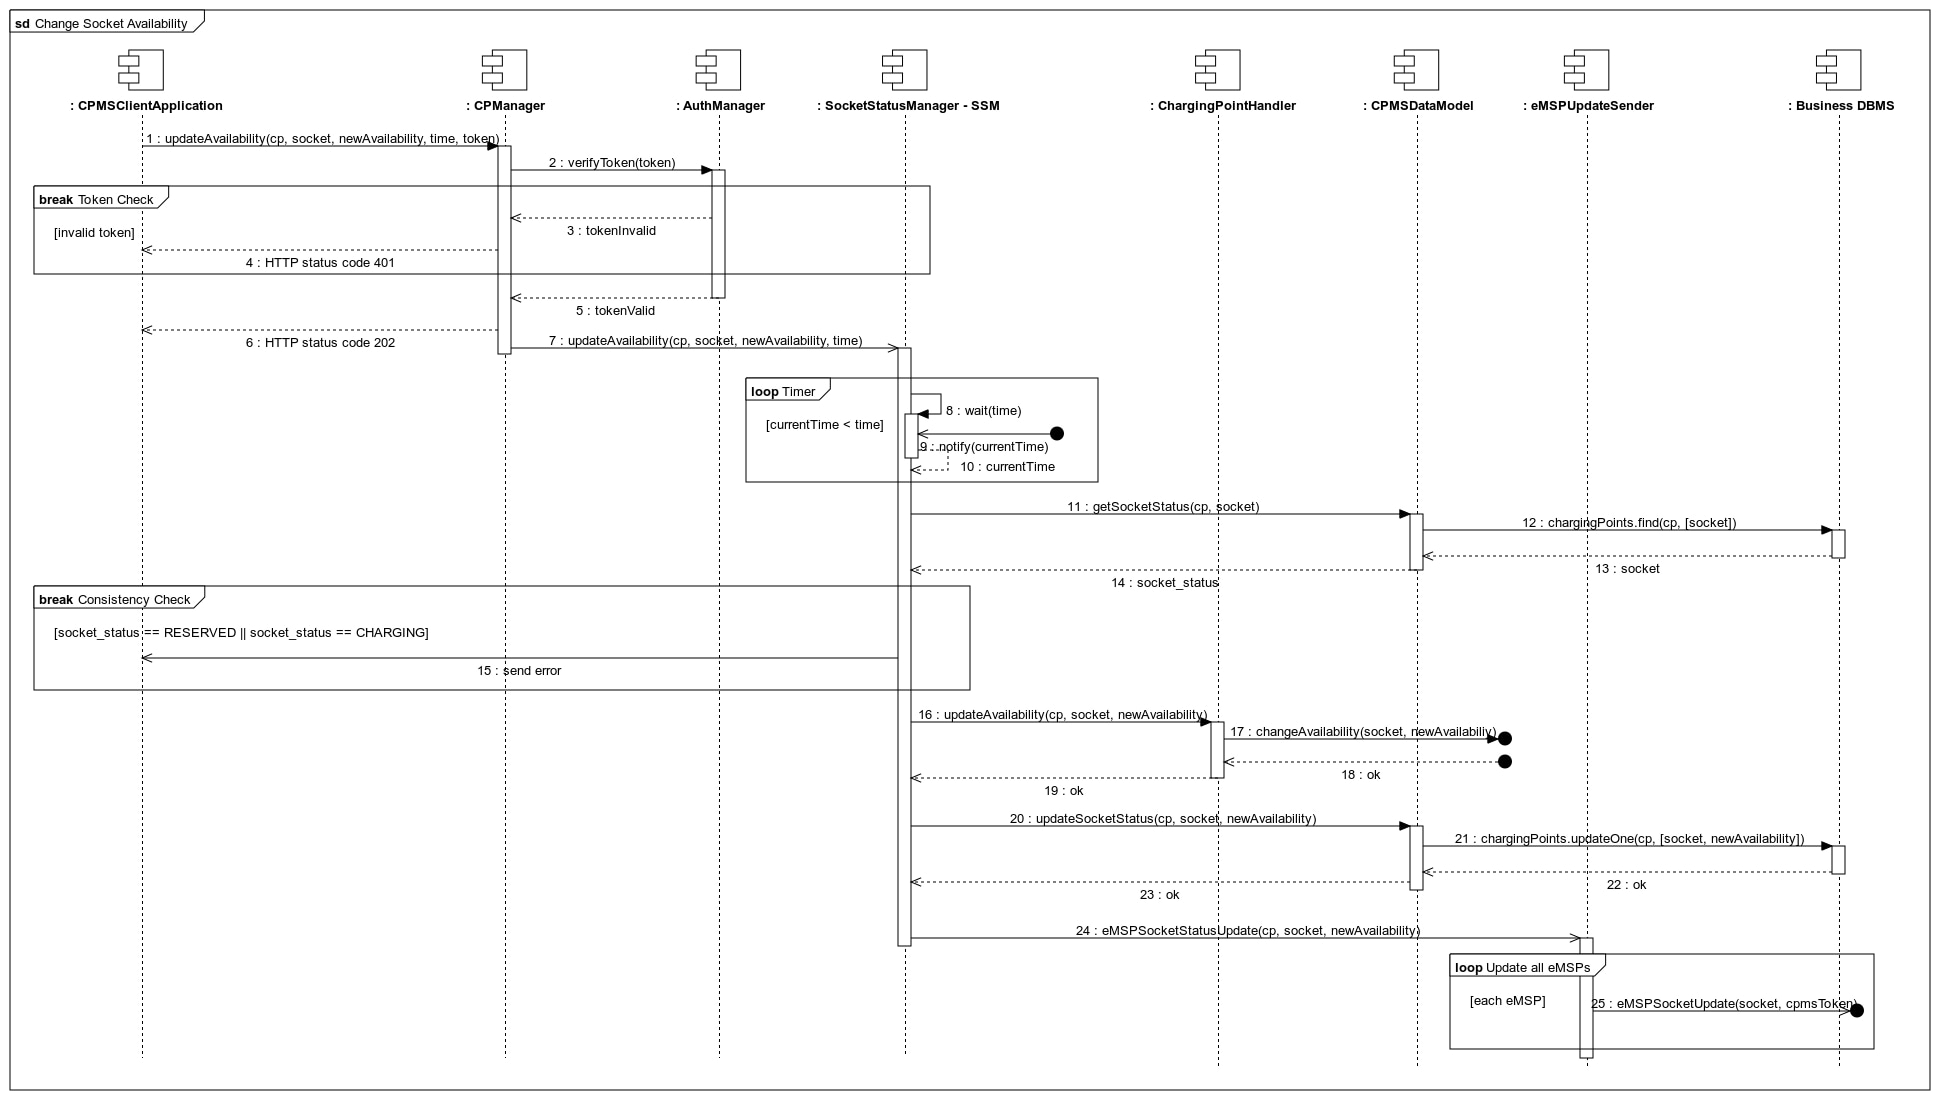
\includegraphics[width=1\textwidth]{Images/sequenceDiagrams/Change Socket Availability.jpg}
    \caption{Change Socket Availabilty}
\end{figure}
When the CPO wants to change the availability of a socket, sets a time at which the new status has to be applied. When the timer is triggered, the system verifies if the socket is free so the status can be changed, otherwise it will abort the change notifying the CPO. Once the socket changes its status, all the eMSPs are notified.

\subsection{Set CP Tariff}
\begin{figure}[H]
    \centering
    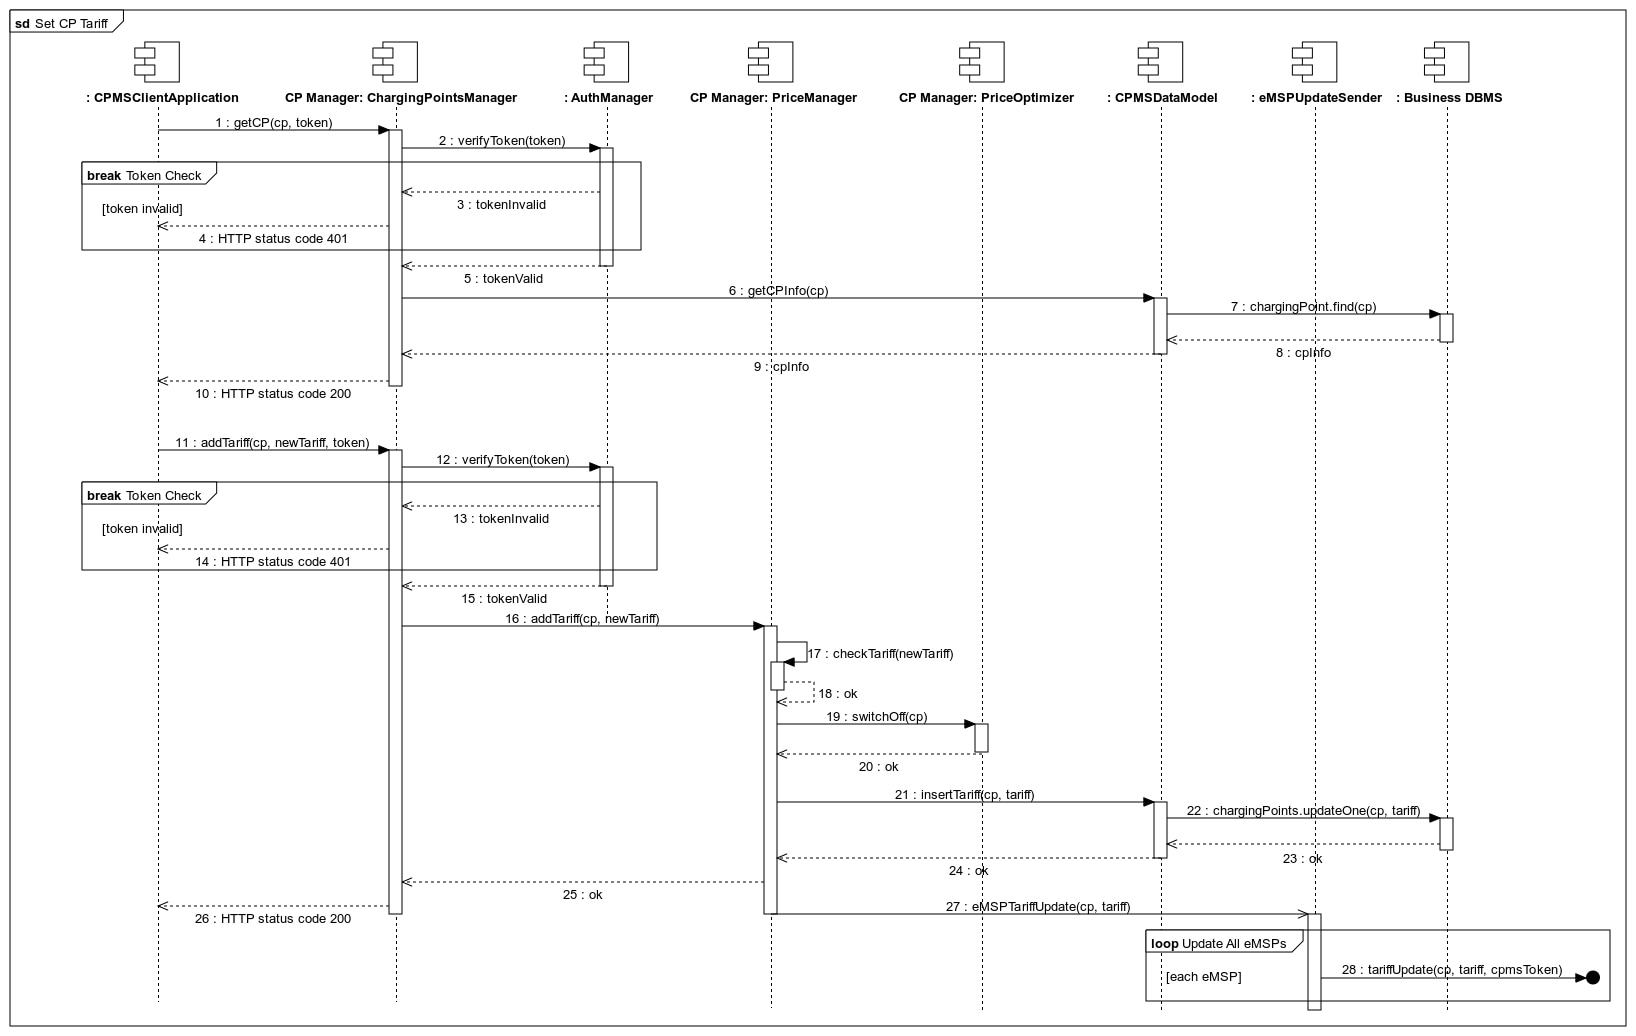
\includegraphics[width=1\textwidth]{Images/sequenceDiagrams/Set CP Tariff.jpg}
    \caption{Set CP Tariff}
\end{figure}
When a CPO wants to set a custom CP Tariff, the Price Optimizer is automatically switched off, then the new price is saved into the DB and all the eMSPs receive the update.

\subsection{Set CP Special Offer}
\begin{figure}[H]
    \centering
    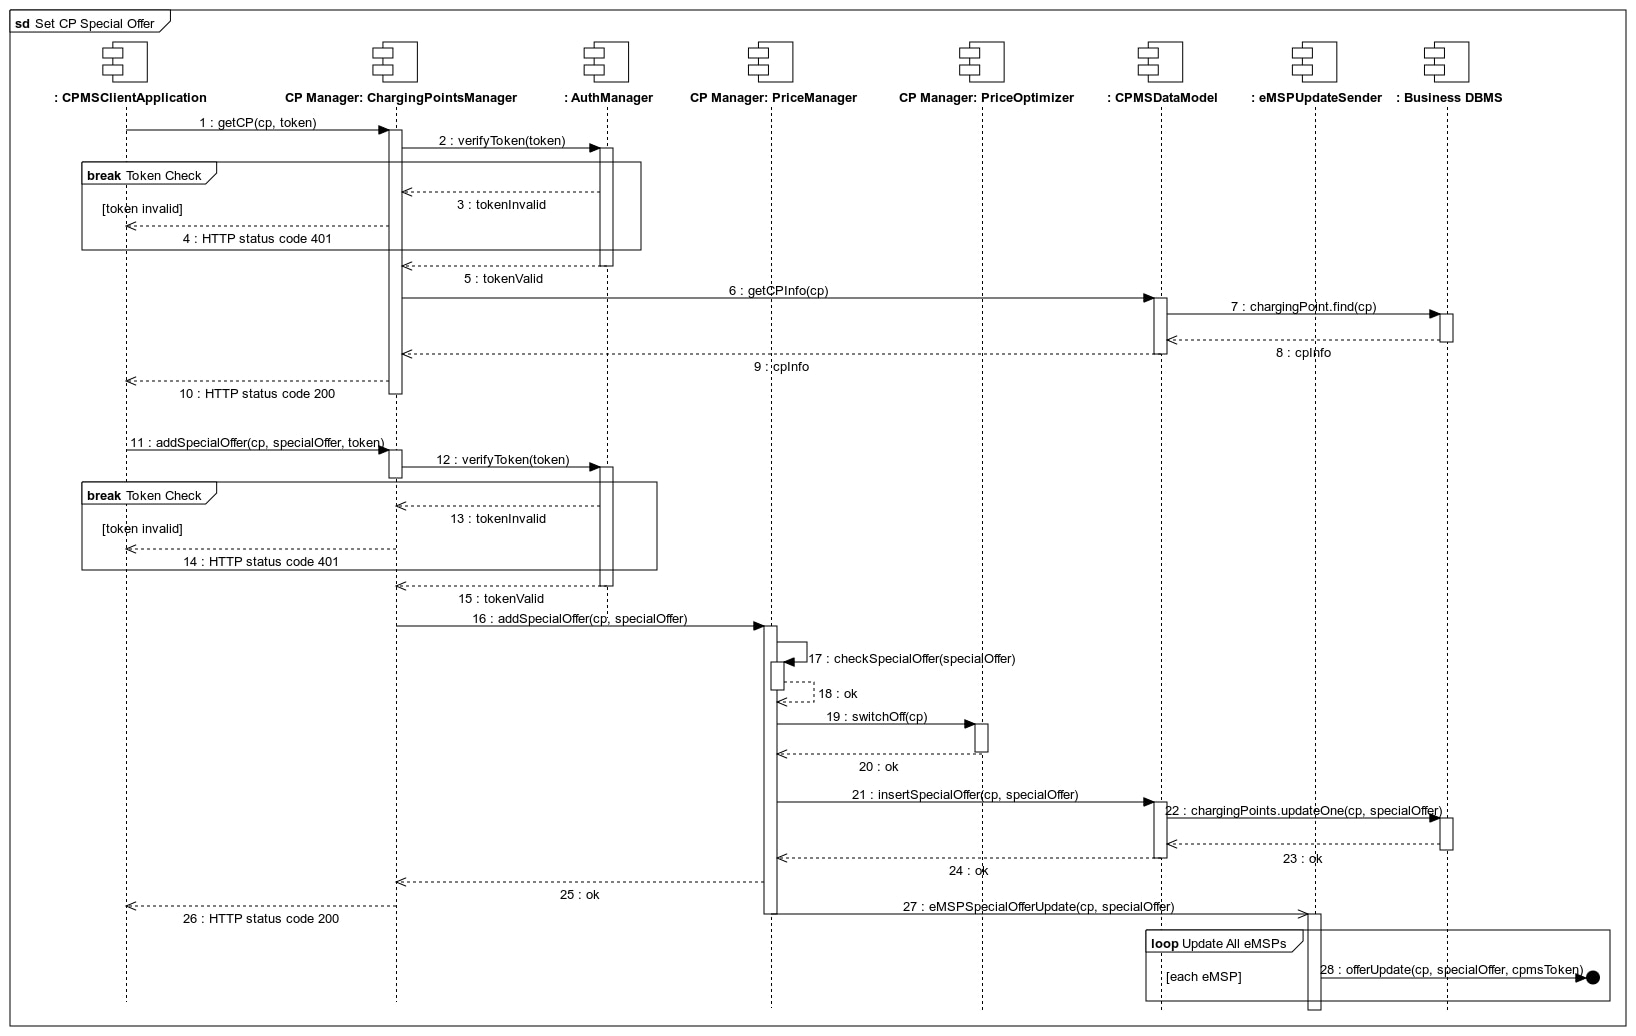
\includegraphics[width=1\textwidth]{Images/sequenceDiagrams/Set CP Special Offer.jpg}
    \caption{Set CP Special Offer}
\end{figure}
As the Set CP tariff but the CPO can rely on different attributes.


\subsection{Remove CP}

\begin{figure}[H]
    \centering
    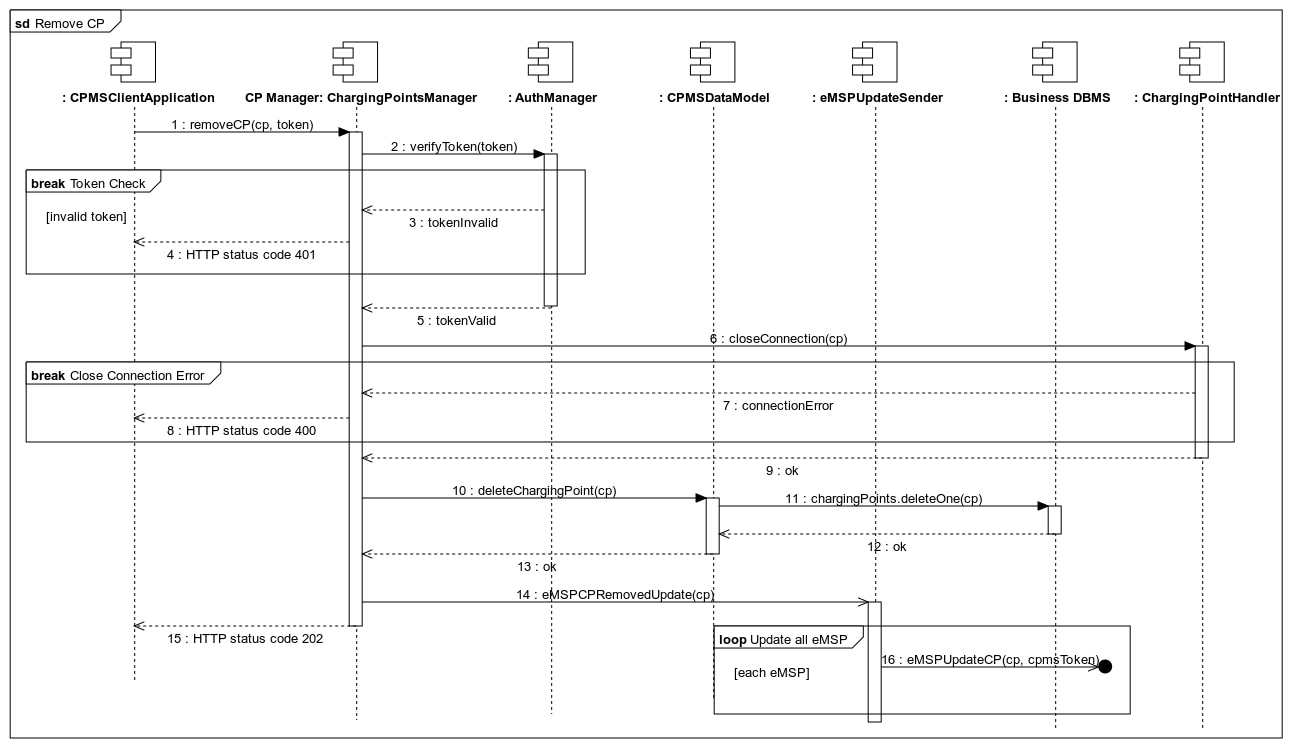
\includegraphics[width=1\textwidth]{Images/sequenceDiagrams/Remove CP.jpg}
    \caption{Remove CP}
\end{figure}
When a CPO wants to remove a CP, the connection between it and the system must be closed before. Once this step is done the system can proceed to remove it from the database, notifying all the eMSPs.

\subsection{Exclude Battery Availability}
\begin{figure}[H]
    \centering
    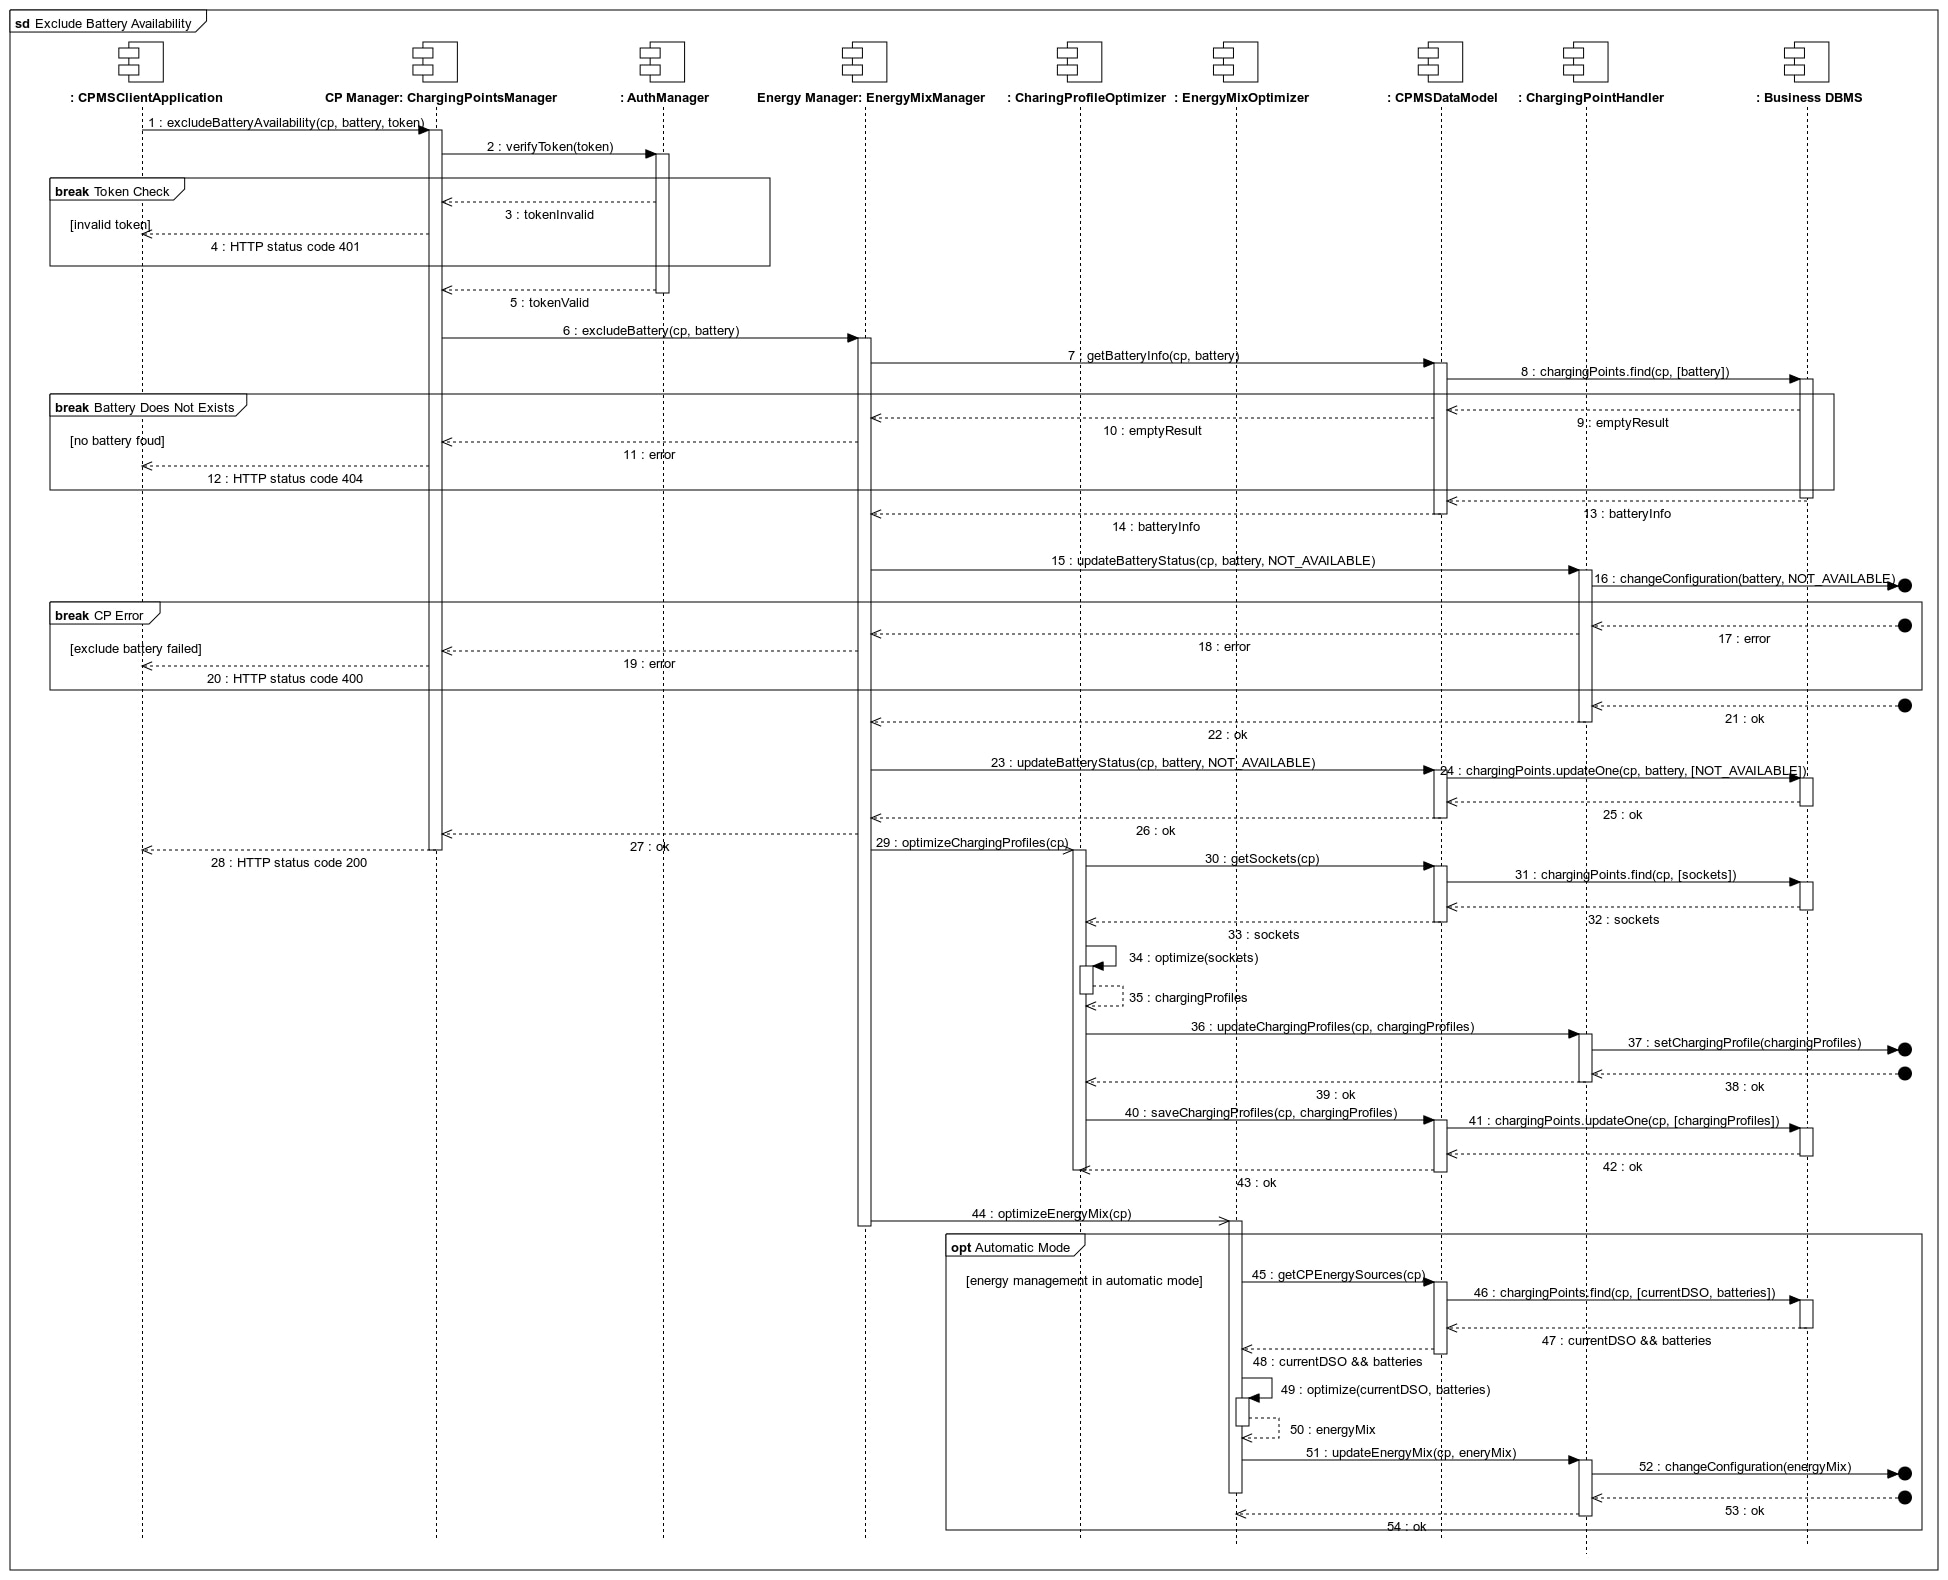
\includegraphics[width=1\textwidth]{Images/sequenceDiagrams/Exclude Battery Availability.jpg}
    \caption{Exclude Battery Availability}
\end{figure}
When we want to exclude the battery from the EnergyMix, an update is sent directly to the CP in order to physically disable the battery. Once it is disabled and the DB is updated with the new state, a confirmation is sent to the client application. In the background, the charging profiles have to be recomputed and updated, as the EnergyMix if it is set in the automatic mode.

\subsection{Change DSO Provider}
\begin{figure}[H]
    \centering
    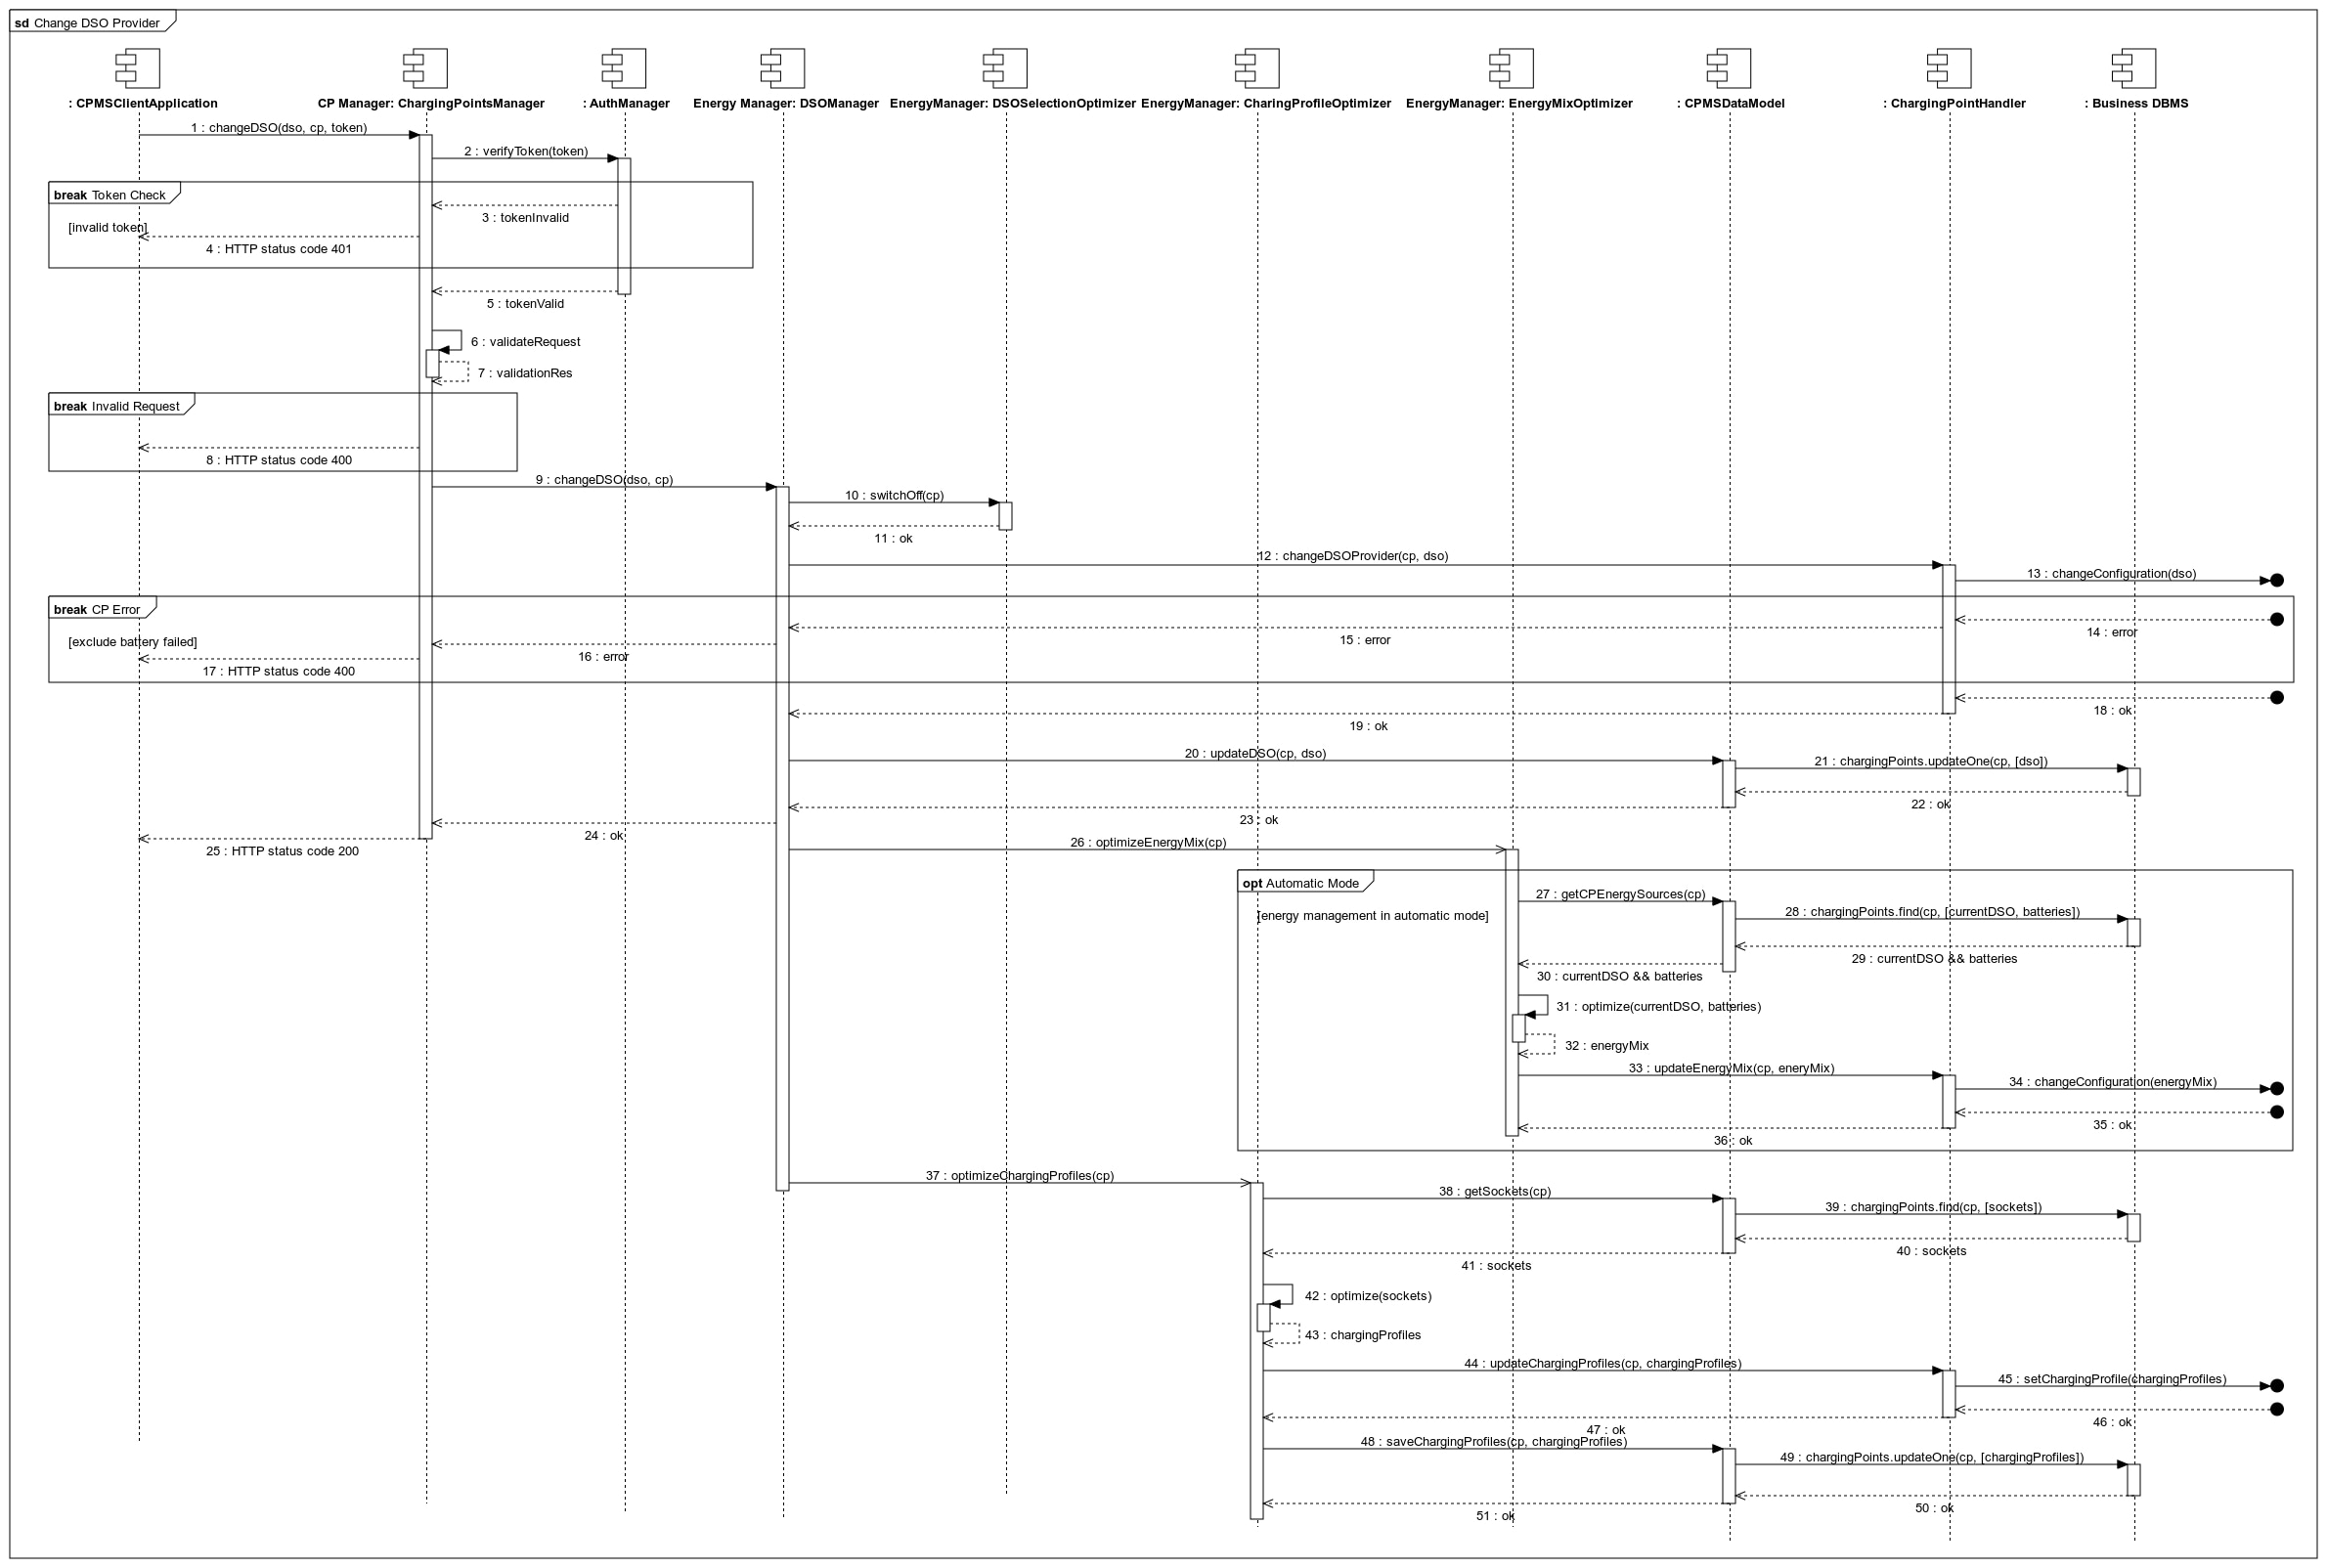
\includegraphics[width=1\textwidth]{Images/sequenceDiagrams/Change DSO Provider.jpg}
    \caption{Change DSO Provider}
\end{figure}
Sometimes the CPO wants to manually select the DSO, in this case, a request is sent and the DSOSelectionOptimizer is automatically switched off. The request is then sent to the CP that switches to the given DSO and then the database is updated returning a success message to the client. In the background, the charging profiles have to be recomputed and updated, as the EnergyMix if it is set in the automatic mode.

\subsection{Toggle Tariff Optimizer}
\begin{figure}[H]
    \centering
    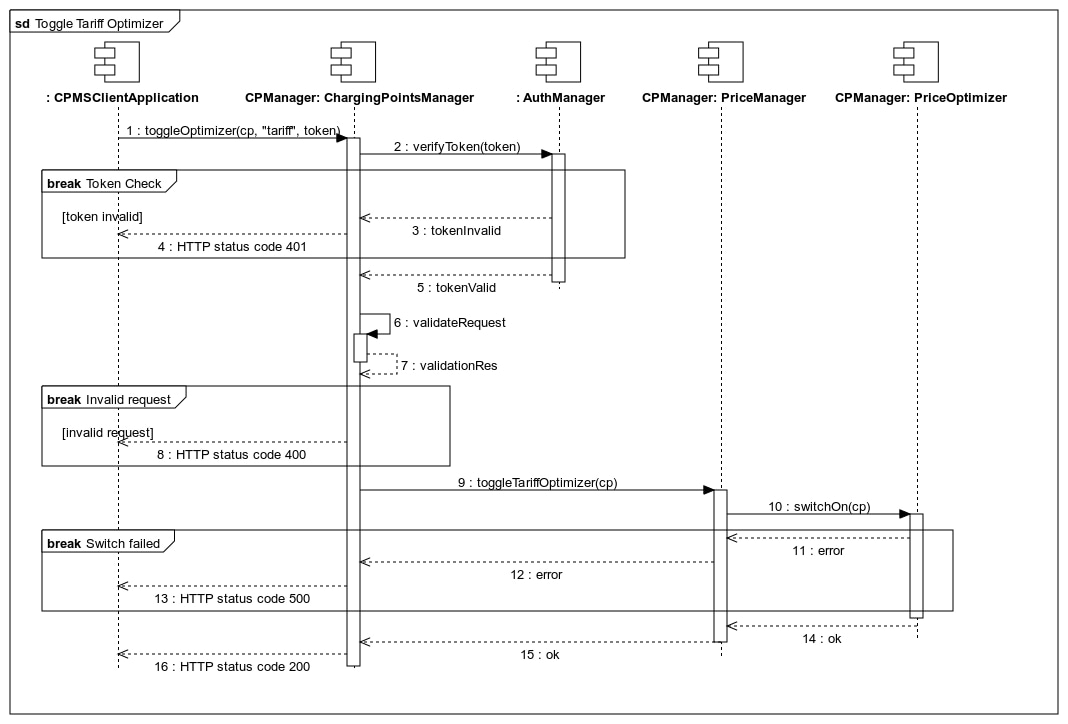
\includegraphics[width=1\textwidth]{Images/sequenceDiagrams/Toggle Tariff Optimizer.jpg}
    \caption{Toggle Tariff Optimizer}
\end{figure}
The CPO can manually switch off or on (based on the last status) the TariffOptimizer. If it's off the last tariff is the valid one, if it's on the new optimal tariffs are computed and applied.

\subsection{Toggle DSO Selection Optimizer}
\begin{figure}[H]
    \centering
    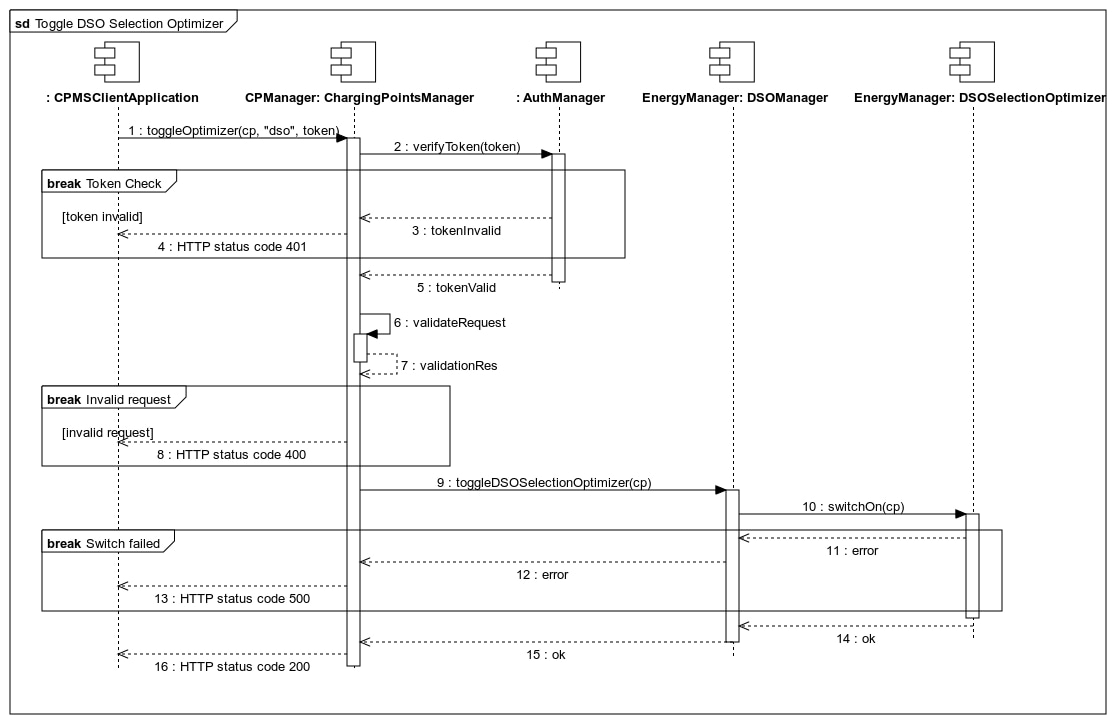
\includegraphics[width=1\textwidth]{Images/sequenceDiagrams/Toggle DSO Selection Optimizer.jpg}
    \caption{Toggle DSO Selection Optimizer}
\end{figure}
The CPO can manually switch off or on (based on the last status) the DSOSelectionOptimizer. If it's off the last DSO is the valid one, if it's on the new optimal DSO is computed and selected.

\subsection{Toggle Energy Mix Optimizer}
\begin{figure}[H]
    \centering
    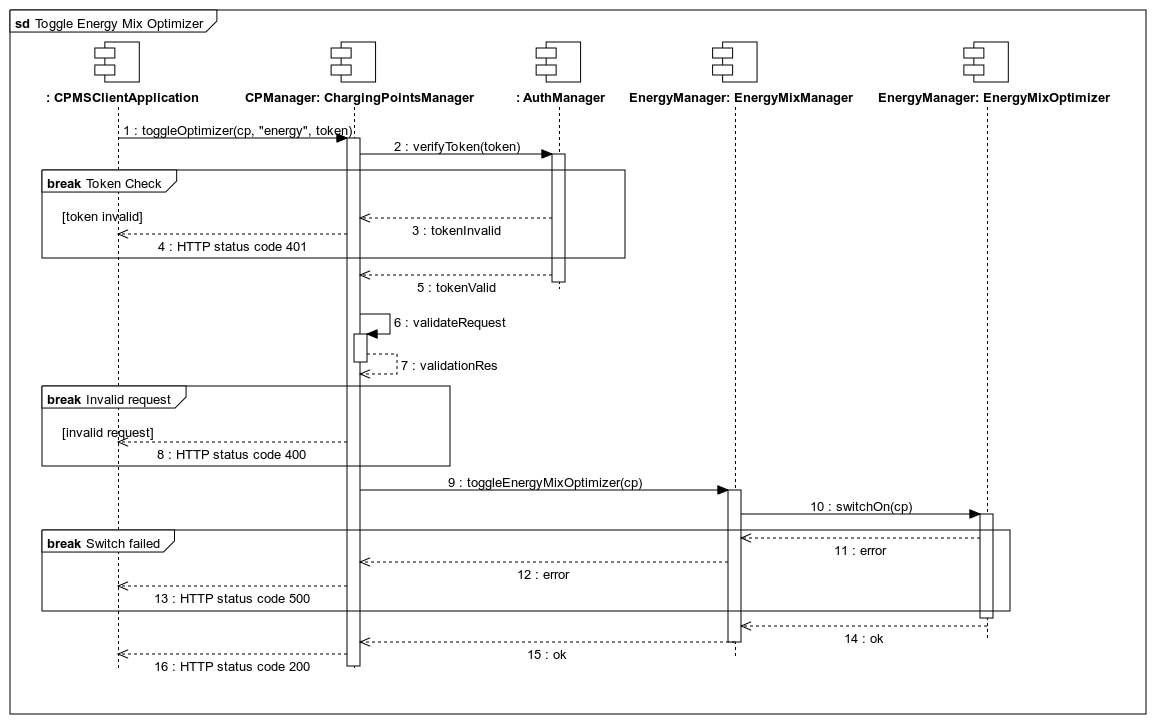
\includegraphics[width=1\textwidth]{Images/sequenceDiagrams/Toggle Energy Mix Optimizer.jpg}
    \caption{Toggle Energy Mix Optimizer}
\end{figure}
The CPO can manually switch off or on (based on the last status) the EnergyMixOptimizer. If it's off the last energy mix is the valid one, if it's on the new optimal energy mix is computed and applied.

\newpage
\section{Component Interfaces}

\subsection{eMSP}

\begin{figure}[H]
    \centering
    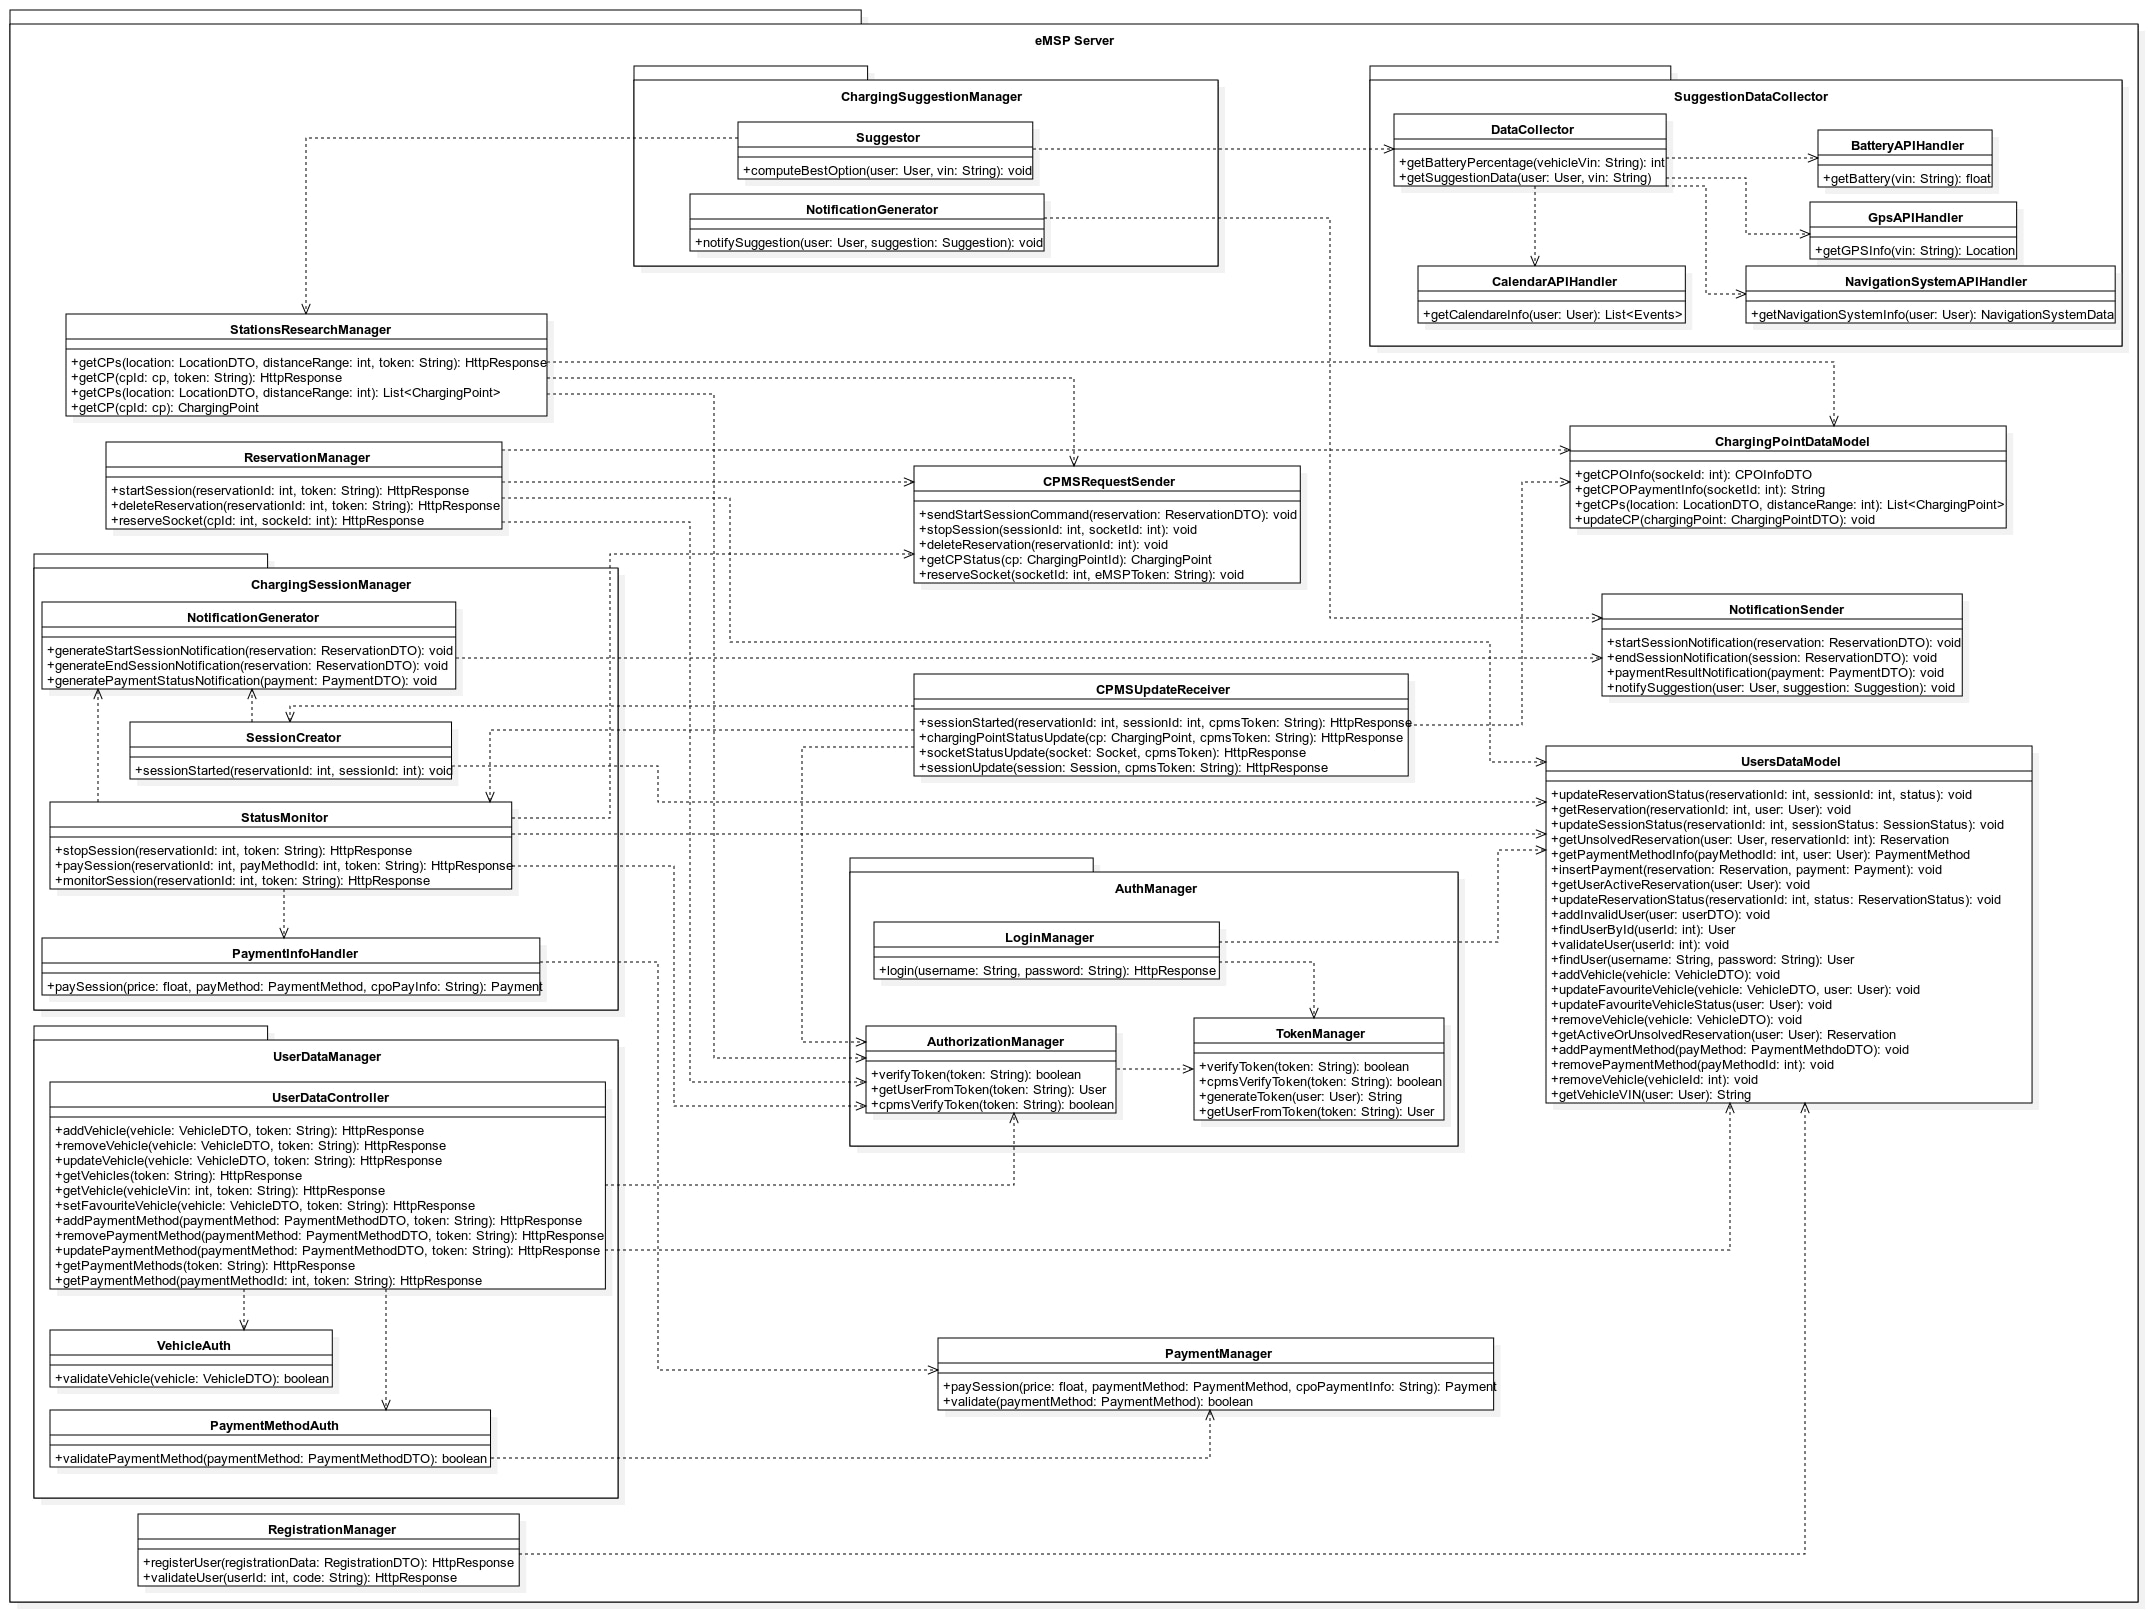
\includegraphics[width=1\textwidth]{Images/component/Component Interfaces eMSP.jpg}
    \caption{eMSP Server Component Interfaces}
    \label{fig:emsp-interfaces}
\end{figure}

\subsection{CPMS}

\begin{figure}[H]
    \centering
    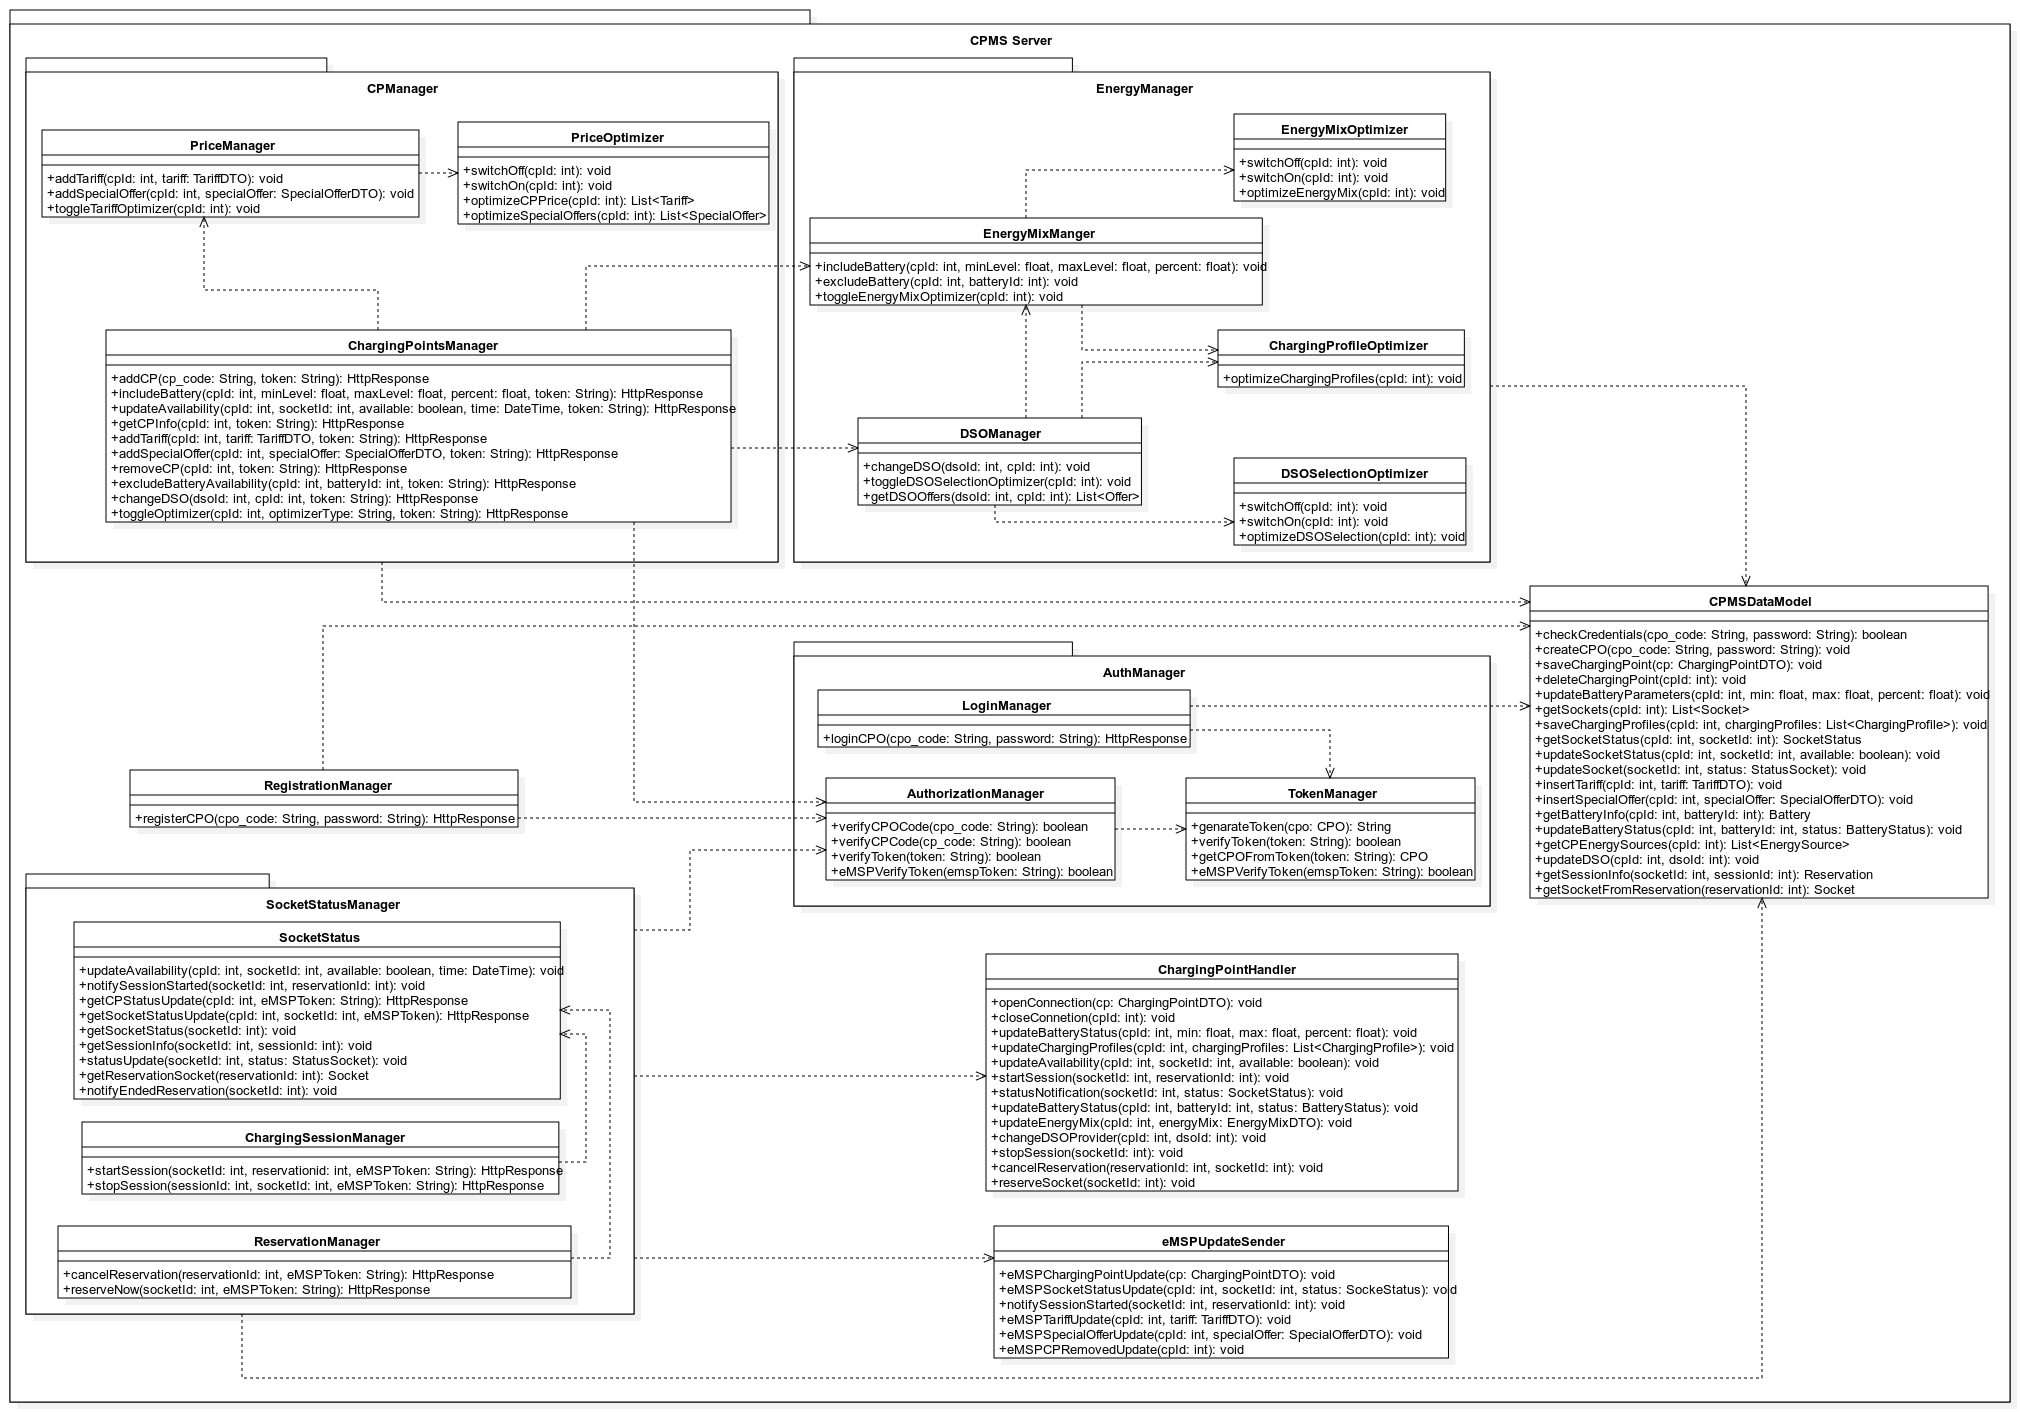
\includegraphics[width=1\textwidth]{Images/component/CPMS Component Interfaces.jpg}
    \caption{CPMS Server Component Interfaces}
    \label{fig:cpms-interfaces}
\end{figure}

\section{Selected Architectural Styles and Patterns}

\begin{itemize}
    \item \textbf{RESTful API}: REST (Representational State Transfer) is a stateless client-server software architectural style that defines a set of constraints and properties for creating web services. RESTful APIs use HTTP requests (GET, POST, PUT and DELETE) to retrieve data or to perform actions, HTTP response codes to indicate the outcome of the request, URLs to identify resources, and HTTP headers to provide additional information about the request or the response. Both the eMSP Server and the CPMS Server is designed to provide a RESTsul API to clients.
    \item \textbf{Three-Tier Architecture}: as previously mentioned, both the CPMS and the eMSP follow the three-tier architecture. The three-tier architecture allows scaling of the business logic tier and the data storage tier independently, which makes it easier to handle changes in workload. In addition, it is easy to troubleshoot and maintain the application since it is easy to change a tier without affecting the others.
    %\item \textbf{Microservices}
    \item \textbf{Stateless Component}: the application server components, for both eMSP and CPMS, do not have any internal state but they save all the information in the database. In this way, performance is improved since there is no session information to retrieve when new requests arrive from the client. Each component is responsible for performing a specific function and communicates with other components through well-defined interfaces. This allows the components to be tested independently and makes the overall system easier to maintain and evolve.
    \item \textbf{Distributed Application}: both the CPMS and the eMSP applications are divided into multiple independent components that provide a certain function. In particular, Layer-based decomposition, which divides the application into separate logical layers was used. In addition, components are designed using a Process-based decomposition that focuses on the business processes supported by the application.
\end{itemize}

\section{Other Design Decisions}

\begin{itemize}
    \item \textbf{Thin client}: for both eMSP and CPMS, all the business logic is inside the server side. This means that the clients have to handle only the presentation layer and keep as low information as possible. In this way, the only requirement that clients need to satisfy is having a stable connection, otherwise, the application will not be working as expected.
    \item \textbf{Horizontal scaling}: Horizontal scaling is the practice of adding more machines or instances to a system to increase its capacity and improve its performance. The workload is distributed across multiple machines or instances, rather than being handled by a single, more powerful machine. Horizontal scaling allows a system to handle a larger workload by adding more resources and can also help to improve fault tolerance by providing redundancy. Horizontal scaling is useful for the eMSP Application Server since it helps to handle all the concurrent requests that the eMSP receives.
\end{itemize}

\chapter{User Interface Design}

\section{eMSP Mobile Application}

\begin{figure}[H]
    \centering
    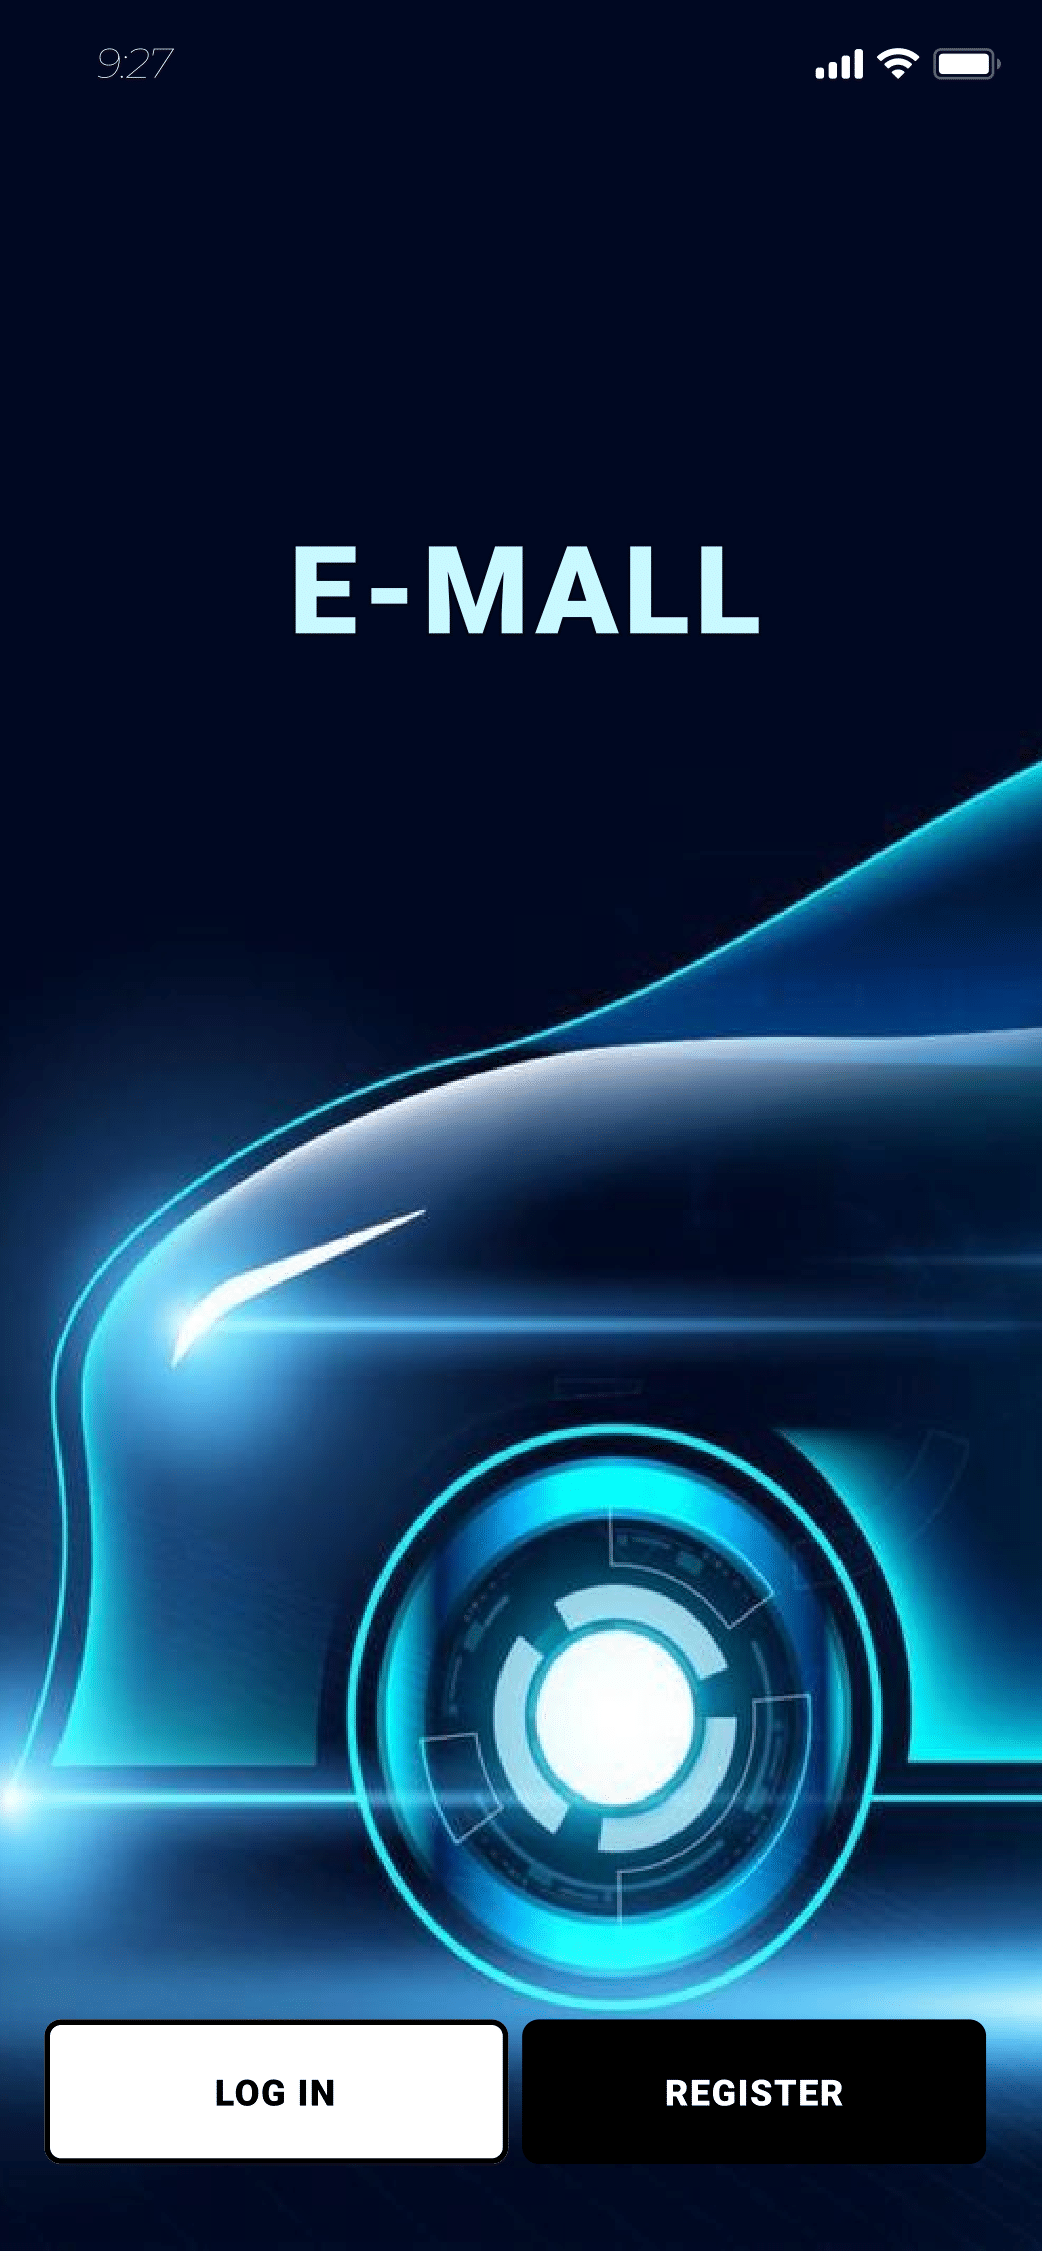
\includegraphics[width=0.5\textwidth]{Images/user-interface/emsp/eMSP (1)-01.png}
    \caption{eMSP initial page}
\end{figure}

\begin{figure}[H]
    \centering
    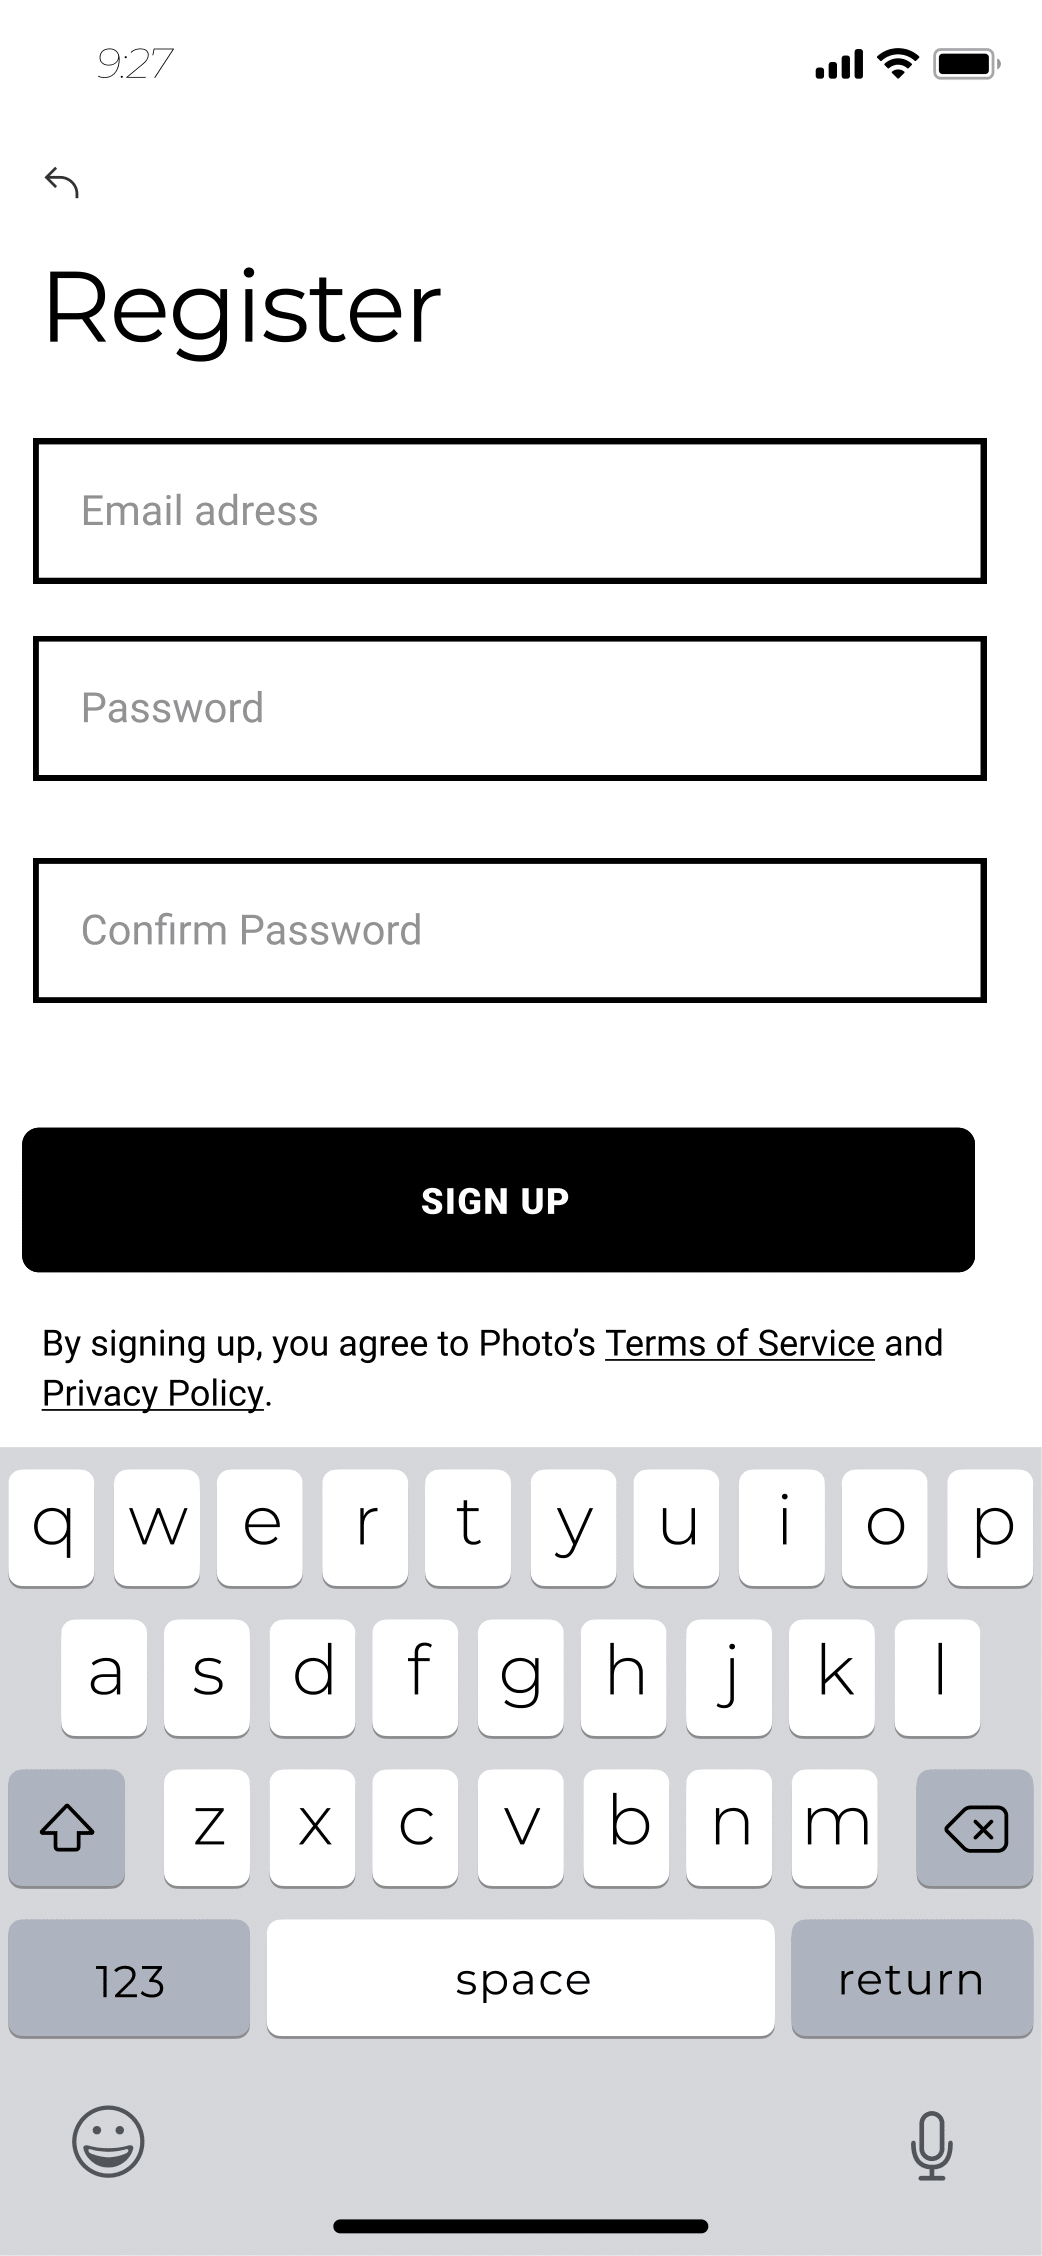
\includegraphics[width=0.6\textwidth]{Images/user-interface/emsp/eMSP (1)-03.png}
    \caption{eMSP registration page}
\end{figure}

\begin{figure}[H]
    \centering
    \includegraphics[width=0.6\textwidth]{Images/user-interface/emsp/eMSP (1)-02.png}
    \caption{eMSP registration code verification page}
\end{figure}

\begin{figure}[H]
    \centering
    \includegraphics[width=0.6\textwidth]{Images/user-interface/emsp/eMSP (1)-04.png}
    \caption{eMSP login page}
\end{figure}

\begin{figure}[H]
    \centering
    \includegraphics[width=0.6\textwidth]{Images/user-interface/emsp/eMSP (1)-05.png}
    \caption{eMSP vehicles information pages}
\end{figure}

\begin{figure}[H]
    \centering
    \includegraphics[width=0.6\textwidth]{Images/user-interface/emsp/eMSP (1)-07.png}
    \caption{eMSP vehicle details page}
\end{figure}

\begin{figure}[H]
    \centering
    \includegraphics[width=0.6\textwidth]{Images/user-interface/emsp/eMSP (1)-06.png}
    \caption{eMSP stations research example}
\end{figure}

\begin{figure}[H]
    \centering
    \includegraphics[width=0.4\textwidth]{Images/user-interface/emsp/eMSP (1)-09.png}
    \caption{eMSP charging point page}
\end{figure}

\begin{figure}[H]
    \centering
    \includegraphics[width=0.6\textwidth]{Images/user-interface/emsp/eMSP (1)-08.png}
    \caption{eMSP confirm reservation page}
\end{figure}

\begin{figure}[H]
    \centering
    \includegraphics[width=0.4\textwidth]{Images/user-interface/emsp/eMSP (1)-12.png}
    \caption{eMSP reservations history page}
\end{figure}

\begin{figure}[H]
    \centering
    \includegraphics[width=0.6\textwidth]{Images/user-interface/emsp/eMSP (1)-10.png}
    \caption{eMSP charging session monitoring page}
\end{figure}

\begin{figure}[H]
    \centering
    \includegraphics[width=0.6\textwidth]{Images/user-interface/emsp/eMSP (1)-11.png}
    \caption{eMSP personal account settings page}
\end{figure}

\begin{figure}[H]
    \centering
    \includegraphics[width=1\textwidth]{Images/user-interface/emsp/eMSP-interactions.jpg}
    \caption{eMSP interactions}
\end{figure}

\section{CPMS Web Application}

\begin{figure}[H]
    \centering
    \includegraphics[width=1\textwidth]{Images/user-interface/cpms/CPMS-2.png}
    \caption{CPMS login page}
\end{figure}

\begin{figure}[H]
    \centering
    \includegraphics[width=1\textwidth]{Images/user-interface/cpms/CPMS-3.png}
    \caption{CPMS home page}
\end{figure}

\begin{figure}[H]
    \centering
    \includegraphics[width=1\textwidth]{Images/user-interface/cpms/CPMS-1.png}
    \caption{CPMS CPO charging points page}
\end{figure}

\begin{figure}[H]
    \centering
    \includegraphics[width=1\textwidth]{Images/user-interface/cpms/CPMS-5.png}
    \caption{CPMS charging point general information page}
\end{figure}

\begin{figure}[H]
    \centering
    \includegraphics[width=0.6\textwidth]{Images/user-interface/cpms/CPMS-4.png}
    \caption{CPMS sockets management page}
\end{figure}

\begin{figure}[H]
    \centering
    \includegraphics[width=1\textwidth]{Images/user-interface/cpms/CPMS-6.png}
    \caption{CPMS DSO offers management page}
\end{figure}

\begin{figure}[H]
    \centering
    \includegraphics[width=1\textwidth]{Images/user-interface/cpms/CPMS-7.png}
    \caption{CPMS charging points statistics page}
\end{figure}

\begin{figure}[H]
    \centering
    \includegraphics[width=1\textwidth]{Images/user-interface/cpms/CPMS-8.png}
    \caption{CPMS energy management page}
\end{figure}

\begin{figure}[H]
    \centering
    \includegraphics[width=1\textwidth]{Images/user-interface/cpms/CPMS-9.png}
    \caption{CPMS tariffs and special offers management page}
\end{figure}

\begin{figure}[H]
    \centering
    \includegraphics[width=1\textwidth]{Images/user-interface/cpms/CPMS-interactions.jpg}
    \caption{CPMS interactions}
\end{figure}

\chapter{Requirements Traceability}

\section{Functional Requirements}

\subsubsection{eMSP components abbreviations for the matrix}
\begin{itemize}
    \item \textbf{ECA:} eMSPClientApplication
    \item \textbf{AM:} AuthManager
    \begin{itemize}
        \item \textbf{LM:} LoginManager
        \item \textbf{TM:} TokenManager
        \item \textbf{ANM:} AuthorizationManager
    \end{itemize}
    \item \textbf{RM:} RegistrationManager
    \item \textbf{UDM:} UserDataManager
    \begin{itemize}
        \item \textbf{UDC:} UserDataController
        \item \textbf{VA:} VehicleAuth
        \item \textbf{PMA:} PaymentMethodAuth
    \end{itemize}
    \item \textbf{SRM:} StationsResearchManager
    \item \textbf{RSM:} ReservationManager
    \item \textbf{CSM:} ChargingSessionManager
    \begin{itemize}
        \item \textbf{SC:} SessionCreator
        \item \textbf{SM:} Status Monitor
        \item \textbf{PIH:} PaymentInfoHandler
        \item \textbf{NG:} NotificationGenerator
    \end{itemize}
    \item \textbf{PM:} PaymentManager
    \item \textbf{CSGM:} ChargingSuggestionManager
    \begin{itemize}
        \item \textbf{SG:} Suggestor
        \item\textbf{BM:} BatteryMonitor
        \item\textbf{NGR:} NotificationGenerator
    \end{itemize}
    \item \textbf{SDC:} SuggestionDataCollector
    \begin{itemize}
        \item \textbf{DC:} DataCollector
        \item \textbf{BAH:} BatteryAPIHandler
        \item \textbf{GAH:} GPSAPIHandler
        \item \textbf{NAH:} NavigationSystemAPIHandler
        \item \textbf{CAH:} CalendarAPIHandler
    \end{itemize}
    \item \textbf{NS:} NotificationSender
    \item \textbf{UM:} UsersDataModel
    \item \textbf{CPM:} ChargingPointDataModel
    \item \textbf{CRS:} CPMSRequestSender
    \item \textbf{CUR:} CPMSUpdateReceiver
\end{itemize}

\subsubsection{CPMS components abbreviations for the matrix}
\begin{itemize}
    \item \textbf{CCA}: CPMSClientApplication
    \item \textbf{AM:} AuthManager
    \item \textbf{RM:} RegistrationManager
    \item \textbf{CM:} CPManager
    \begin{itemize}
        \item \textbf{CPM:} ChargingPointsManager
        \item \textbf{PM:} PriceManager
        \item \textbf{PO:} PriceOptimizer
    \end{itemize}
    \item \textbf{SSM:} SocketStatusManager
    \begin{itemize}
        \item \textbf{SS:} SocketStatus
        \item \textbf{RSM:} ReservationManager
        \item \textbf{CSM:} ChargingSessionManager
    \end{itemize}
    \item \textbf{EM:} EnergyManager
    \begin{itemize}
        \item \textbf{DM:} DSOManager
        \item \textbf{DSO:} DSOSelectionOptimizer
        \item \textbf{EMM:} EnergyMixManager
        \item \textbf{EMO:} EnergyMixOptimizer
        \item \textbf{CPO:} ChargingProfileOptimizer
    \end{itemize}
    \item \textbf{DH:} DSOHandler
    \item \textbf{EUS:} eMSPUpdateSender
    \item \textbf{CPH:} ChargingPointHandler
    \item \textbf{CDM:} CPMSDataModel
\end{itemize}

\subsection{Requirements Matrix}

\begin{xltabular}{\textwidth}{| >{\columncolor{bluepoli!40}}l | X | X |}
\hline
\rowcolor{bluepoli!40}
    \textbf{Requirement} & \textbf{eMSP}& \textbf{CPMS}\T\B\\
\hline

R1 & ECA, RM, UM & \B\\
\hline
 
R2 & ECA, RM, UM & \B\\
\hline

R3 & ECA, AM, LM, TM, UM & \B\\
\hline

R4 & ECA, UDM, UDC, VA, UM, AM, ANM, TM & \B\\
\hline

R5 & ECA, UDM, UDC, VA, AM, ANM, TM & \B\\
\hline

R6 & ECA, UDM, UDC, UM, AM, ANM, TM & \B\\
\hline

R7 & ECA, UDM, UDC, UM, AM, ANM, TM & \B\\
\hline

R8 & ECA, UDM, UDC, PMA, UM, PM, AM, ANM, TM & \B\\
\hline

R9 & ECA, UDM, UDC, PMA, PM, AM, ANM, TM & \B\\
\hline

R10 & ECA, UDM, UDC, UM, AM, ANM, TM & \B\\
\hline

R11 & ECA, RM, UM, AM, ANM, TM & \B\\
\hline

R12 & ECA, RM, UM, AM, ANM, TM & \B\\
\hline

R13 & ECA, RM, CRS & SSM, RSM, CPH, AM \B\\
\hline

R14 & ECA, SRM, CPM, AM, ANM, TM & \B\\
\hline

R15 & ECA, RM, CRS, UM, AM, ANM, TM & SSM, RSM, CPH, CDM, AM \B\\
\hline
  
R16 & ECA, SRM, CPM, UM, AM, ANM, TM & \B\\
\hline

R17 & ECA, RM, CRS, UM, AM, ANM, TM & SSM, RSM, CPH, CDM, AM \B\\
\hline

R18 & ECA, RM, CRS, UM, AM, ANM, TM & SSM, RSM, CPH, CDM, AM \B\\
\hline
  
R19 & ECA, RM, UM, AM, ANM, TM & \B\\
\hline

R20 & ECA & \B\\
\hline

R21 & CSGM, SG, BM, NGR, NS, ECA & \B\\
\hline

R22 & SDC, BAH, DC & \B\\
\hline

R23 & SDC, CAH, DC & \B\\
\hline

R24 & SDC, NAH, DC & \B\\
\hline

R25 & SDC, GAH, DC & \B\\
\hline

R26 & SDC, DC, BAH, GAH, NAH, CAH, CSGM, SG, BM, NGR, ECA & \B\\
\hline

R27 & ECA &\B\\
\hline

R28 & ECA, RM, CRS, UM, AM, ANM, TM & SSM, RSM, CPH, CDM, AM \B\\
\hline

R29 & ECA, CRS, UM, AM, ANM, TM & SSM, SS, RSM, CPH, CDM, EUS, AM \B\\
\hline

R30 & ECA, CRS, UM, AM, ANM, TM & SSM, SS, RSM, CPH, CDM, EUS, AM \B\\
\hline

R31 & ECA, RM, CSM, SC, AM, ANM, TM, UM, CRS & AM, SSM, SS, CSM, CDM, CPH, EUS \B\\
\hline

R32 & ECA, CSM, SM, AM, ANM, TM, UM & AM, SSM, SS, CSM, CPH\B\\
\hline

R33 & ECA, RM, CSM, SC, AM, ANM, TM, UM, CRS & AM, SSM, SS, CSM, CDM, CPH, EUS \B\\
\hline

R34 & ECA, CSM, SM, PIH, PM, UM, CPM, AM, ANM, TM & \B\\
\hline

R35 & ECA, CSM, SM, PIH, PM, UM, CPM AM, ANM, TM & \B\\
\hline

R36 & ECA, CSM, SM, PIH, PM, UM, CPM AM, ANM, TM & \B\\
\hline
    
R37 & ECA, CSM, SM, PIH, PM, UM, CPM AM, ANM, TM, NG, NS & \B\\
\hline
    
R38 & ECA, CSM, SM, PIH, PM, UM, CPM AM, ANM, TM & \B\\
\hline
    
R39 & ECA & \B\\
\hline

R40 & ECA, CSM, SM, AM, ANM, TM, UM, CRS & AM, SSM, SS, CSM, CDM, CPH, EUS \B\\
\hline

R41 & CUR, AM, ANM, TM, CSM, NG, NS, ECA & CPH, SSM, SS, EUS \B\\
\hline

R42 & ECA, CSM, SM, AM, ANM, TM, UM, CRS & AM, SSM, SS, CSM, CDM, CPH, EUS \B\\
\hline

R43 & CUR, AM, ANM, TM, CPM & CCA, CM, CPM, EUS \B\\
\hline
    
R44 & ECA, CSM, SM, AM, ANM, TM, UM & AM, SSM, SS, CSM, CPH \B\\
\hline

R45 & CUR, AM, ANM, TM, CPM & SSM, RSM, CPH, EUS \B\\
\hline
 
R46 & CUR, AM, ANM, TM, CPM & SSM, RSM, CPH, EUS \B\\
\hline

R47 &  & SSM, RSM, AM, CPH, CDM \B\\
\hline

R48 & CUR, AM, ANM, TM, CPM & SSM, SS, EUS, \B\\
\hline

R49 &  & SSM, RSM, AM, CPH, CDM \B\\
\hline

R50 & & SSM, CSM, AM, CPH, CDM \B\\
\hline

R51 & & CCA, RM, AM, CDM \B\\
\hline

R52 & & AM \B\\
\hline

R53 & & CCA, AM, CDM \B\\
\hline

R54 & & AM \B\\
\hline

R55 & & CM, CPM, CPH, EUS, CDM \B\\
\hline

R56 & CUR, AM, ANM, TM, CPM & CM, CPM, CPH, EUS, CDM \B\\
\hline

R57 & & CPH \B\\
\hline

R58 & & CCA, AM, CM, CPM, CPH, CDM \B\\
\hline

R59 & & CCA, AM, CM, CPM, CPH, CDM, SSM, SS, EUS \B\\
\hline

R60 & & CCA, AM, CM, CPM, CPH, SSM, SS \B\\
\hline

R61 & & CM, PM, PO, EUS, CDM \B\\
\hline

R62 & & CCA, AM, CM, CPM, PM, EUS, CDM \B\\
\hline

R63 & & CCA, AM, CM, CPM, PM, EUS, CDM \B\\
\hline
    
R64 & & CM, PM, PO, EUS, CDM \B\\
\hline

R65 & & CM, CPM, CPH, EUS, CDM \B\\
\hline

R66 & CUR, AM, ANM, TM, CPM & CM, CPM, CPH, EUS, CDM \B\\
\hline

R67 & & CCA, AM, CM, CPM, CDM, DH \B\\
\hline

R68 & & DH, CDM \B\\
\hline

R69 & & EM, DM, DSO, DH, CPH, CDM \B\\
\hline

R70 & & CCA, AM, EM, DM, DH, CPH, CDM \B\\
\hline

R71 & & CCA, AM, EM, DM, DSO, CM, CPM \B\\
\hline
    
R72 & & CCA, AM, EM, EMM, EMO, CM, CPM \B\\
\hline

R73 & & SSM, CSM, AM, CPH \B\\
\hline
    
R74 & & CCA, AM, EM, EMM, CPH, CDM, CM, CPM \B\\
\hline 

R75 & & EM, EMO \B\\
\hline

R76 & & CCA, AM, EM, EMM, CM, CPM \B\\
\hline

R77 & & EM, CPO, CPH, CDM \B\\
\hline

R78 & & EM, EMM, EMO, CPH, CDM \B\\
\hline

R79 & & CCA, AM, CM, CPM, EM, EMM, EMO, CPH, CDM \B\\
\hline

R80 & & CM, CPM, EM, EMM, EMO, CPH \B\\
\hline

R81 & CUR, AM, ANM, TM, CPM & CCA, CM, CPM, EUS \B\\
\hline

R82 & & EM, DM, DSO, CPO, CPH, CDM \B\\
\hline

R83 & & CCA, AM, CM, CPM, PM, PO, CDM \B\\
\hline
\end{xltabular}

\section{Non Functional Requirements}

\begin{itemize}
    \item \textbf{Reliability and Availability}: these constraints have been accomplished by introducing replication of the server application of the eMSP in several clones. Indeed, when a clone is down, the other nodes in parallel can continue working; therefore, the system remains available as long as at least one clone is working, so the probability of the whole system to brake is very low.
    \item \textbf{Maintainability}: the software is designed through small modules. In this way, the software will be easy to maintain since small changes to some modules will not affect the other modules. In addition, the separation in the Three-Tier Architecture allows for maintaining independently the three tiers.
    \item \textbf{Portability}: the eMSP will be developed for both IOS and Android operating systems and therefore will be available in all mobile devices that contain those operating systems, which constitute the vast majority of the devices. On the other hand, the CPMS will be developed as a web application, and therefore it will be available for all devices that have a web browser installed.
    \item \textbf{Security}: all the communications between server and clients are done using HTTPS, which provides secure communication between the two entities. In addition, clients must use a token (that will have an expiration time) assigned by the server to authenticate for accessing services and resources. Also, the communication between eMSPs and CPMSs is done using tokens to authenticate them.
    \item \textbf{Performance}: the performance requirements have been handled in the following ways
        \begin{itemize}
            \item On the eMSP side, the Charging Points database is useful to maintain a cache of the charging point location and status, therefore searching for stations around a certain position does not need to pass through the CPMS but can rely on this source of information. In addition, the choice of MongoDB for this database permits to automatically partition of the data using a certain key (e.g. the position) and this can speed up the queries used for retrieving charging points in station research. Finally, the horizontal scaling technique for the eMSP Server is useful to handle many concurrent requests. In this view, a RESTful API helps since it provides stateless communication, therefore the client requests do not have to be assigned always to the same replica.
            \item On the CPMS side, there are two important performance aspects to be considered: the high amount of updates arriving from the CPs and the fact that the CPMS must send to the eMSPs the updates on the status of the sockets as soon as possible. These are handled with two dedicated components, i.e. the Charging Point Handler, which has the only responsibility of managing the communication with the charging points, and the eMSP Update Sender, which is only responsible to update all the eMSPs with information about the charging points. These two components, if needed in the future, might also run on a different machine or in order to improve the performance of the CPMS.
        \end{itemize}
\end{itemize}

\chapter{Implementation, Integration and Test Plan}

In this section, the plans to follow for the implementation and testing of the system are described.

\section{Implementation}
The implementation of the two systems will proceed in parallel reusing some of the components (as the AuthManager) in both. A bottom-up approach can be a good choice cause we want to develop a system that is composed of modular components and we want to ensure that each component is working correctly before integrating them.

There are several benefits to using a bottom-up approach:
\begin{enumerate}
    \item It allows for a more incremental development process, which can be less risky and more manageable than trying to develop the entire system all at once.
    \item It allows us to test and debug each component individually, which can make it easier to identify and fix issues.
    \item It can be easier to make changes to individual components without affecting the rest of the system.
    \item It can be easier to reuse components in other projects or systems.
\end{enumerate}

\section{Integration and Test Plan}

A bottom-up strategy was used for generating the following graphics. This approach is been chosen in order to test the components as soon as their development is completed, this gives us the advantage of incremental testing when adding components. The drivers in the schemas are used for simulating the external calls that the server receives out of our domain.\\\\
Following we have an example of an integration test of the components needed by the ReservationManager, this approach has been applied for every component in order to obtain the integration of the systems and the threads that all together provide a user-visible program feature.

\begin{figure}[H]
    \centering
    \includegraphics[width=0.3\textwidth]{Images/test/Thread example/2.jpg}
    \caption{Integration test of DBMS and model component.}
\end{figure}

\begin{figure}[H]
    \centering
    \includegraphics[width=0.3\textwidth]{Images/test/Thread example/3.jpg}
    \caption{integrating the CPMSRequestSender.}
\end{figure}

\begin{figure}[H]
    \centering
    \includegraphics[width=0.25\textwidth]{Images/test/Thread example/5.jpg}
    \caption{Integration test of DBMS and model component.}
\end{figure}

\begin{figure}[H]
    \centering
    \includegraphics[width=0.25\textwidth]{Images/test/Thread example/6.jpg}
    \caption{Integrating the AuthManager.}
\end{figure}

\begin{figure}[H]
    \centering
    \includegraphics[width=0.4\textwidth]{Images/test/Thread example/7.jpg}
    \caption{The final integration of the ReservationManager.}
\end{figure}

\begin{figure}[H]
    \centering
    \includegraphics[width=1\textwidth]{Images/test/test-eMSP-thread.jpg}
    \caption{The final integration of the system with all the threads, eMSPClientApplication.}
\end{figure}

\begin{figure}[H]
    \centering
    \includegraphics[width=1\textwidth]{Images/test/test-CPMS-thread.jpg}
    \caption{The final integration of the system with all the threads, CPMSClientApplication.
}
\end{figure}

\chapter{Effort Spent}

\section{Lorenzo Ferretti}

\begin{table}[H]
    \centering 
    \begin{tabular}{|l|c|}
    \hline
    \rowcolor{bluepoli!40}
    \textbf{Task} & \textbf{Hours Spent} \T\B \\
    \hline
    Introduction & 2 \T\B \\
    \hline
    Architectural Design & 25\T\B \\
    \hline
    User Interface Design & 12\T\B \\
    \hline
    Requirement Traceability & 1\T\B \\
    \hline
    Implementation, Integration and Test Plan & 5\T\B \\
    \hline
    \end{tabular}
\end{table}

\section{Lorenzo Manoni}

\begin{table}[H]
    \centering 
    \begin{tabular}{|l|c|}
    \hline
    \rowcolor{bluepoli!40}
    \textbf{Task} & \textbf{Hours Spent} \T\B \\
    \hline
    Introduction & 2\T\B \\
    \hline
    Architectural Design & 25\T\B \\
    \hline
    User Interface Design & 5\T\B \\
    \hline
    Requirement Traceability & 3\T\B \\
    \hline
    Implementation, Integration and Test Plan & 10\T\B \\
    \hline
    \end{tabular}
\end{table}

\section{Carlo Sgaravatti}

\begin{table}[H]
    \centering 
    \begin{tabular}{|l|c|}
    \hline
    \rowcolor{bluepoli!40}
    \textbf{Task} & \textbf{Hours Spent} \T\B \\
    \hline
    Introduction & 5\T\B \\
    \hline
    Architectural Design & 35\T\B \\
    \hline
    User Interface Design & 2\T\B \\
    \hline
    Requirement Traceability & 4\T\B \\
    \hline
    Implementation, Integration and Test Plan & 2\T\B \\
    \hline
    \end{tabular}
\end{table}

\cleardoublepage

\end{document}
